% Generated by Sphinx.
\documentclass[a4paper,12pt,ngerman]{manual}
\usepackage[utf8]{inputenc}
\usepackage[T1]{fontenc}
\usepackage{babel}
\usepackage{times}
\usepackage[Sonny]{fncychap}
\usepackage{longtable}
\usepackage{sphinx}


\title{Plone Benutzerhandbuch}
\date{03. 04. 2010}
\release{4.0}
\author{Jan Ulrich Hasecke, Thomas Lotze}
\newcommand{\sphinxlogo}{\includegraphics{plone-logo-48.png}\par}
\renewcommand{\releasename}{Release}
\makeindex
\makemodindex

\makeatletter
\def\PYG@reset{\let\PYG@it=\relax \let\PYG@bf=\relax%
    \let\PYG@ul=\relax \let\PYG@tc=\relax%
    \let\PYG@bc=\relax \let\PYG@ff=\relax}
\def\PYG@tok#1{\csname PYG@tok@#1\endcsname}
\def\PYG@toks#1+{\ifx\relax#1\empty\else%
    \PYG@tok{#1}\expandafter\PYG@toks\fi}
\def\PYG@do#1{\PYG@bc{\PYG@tc{\PYG@ul{%
    \PYG@it{\PYG@bf{\PYG@ff{#1}}}}}}}
\def\PYG#1#2{\PYG@reset\PYG@toks#1+\relax+\PYG@do{#2}}

\def\PYG@tok@gu{\let\PYG@bf=\textbf\def\PYG@tc##1{\textcolor[rgb]{0.50,0.00,0.50}{##1}}}
\def\PYG@tok@gt{\def\PYG@tc##1{\textcolor[rgb]{0.00,0.25,0.82}{##1}}}
\def\PYG@tok@gs{\let\PYG@bf=\textbf}
\def\PYG@tok@gr{\def\PYG@tc##1{\textcolor[rgb]{1.00,0.00,0.00}{##1}}}
\def\PYG@tok@cm{\let\PYG@it=\textit\def\PYG@tc##1{\textcolor[rgb]{0.25,0.50,0.56}{##1}}}
\def\PYG@tok@vg{\def\PYG@tc##1{\textcolor[rgb]{0.73,0.38,0.84}{##1}}}
\def\PYG@tok@m{\def\PYG@tc##1{\textcolor[rgb]{0.13,0.50,0.31}{##1}}}
\def\PYG@tok@mh{\def\PYG@tc##1{\textcolor[rgb]{0.13,0.50,0.31}{##1}}}
\def\PYG@tok@go{\def\PYG@tc##1{\textcolor[rgb]{0.19,0.19,0.19}{##1}}}
\def\PYG@tok@ge{\let\PYG@it=\textit}
\def\PYG@tok@gd{\def\PYG@tc##1{\textcolor[rgb]{0.63,0.00,0.00}{##1}}}
\def\PYG@tok@il{\def\PYG@tc##1{\textcolor[rgb]{0.13,0.50,0.31}{##1}}}
\def\PYG@tok@cs{\def\PYG@tc##1{\textcolor[rgb]{0.25,0.50,0.56}{##1}}\def\PYG@bc##1{\colorbox[rgb]{1.00,0.94,0.94}{##1}}}
\def\PYG@tok@cp{\def\PYG@tc##1{\textcolor[rgb]{0.00,0.44,0.13}{##1}}}
\def\PYG@tok@gi{\def\PYG@tc##1{\textcolor[rgb]{0.00,0.63,0.00}{##1}}}
\def\PYG@tok@gh{\let\PYG@bf=\textbf\def\PYG@tc##1{\textcolor[rgb]{0.00,0.00,0.50}{##1}}}
\def\PYG@tok@ni{\let\PYG@bf=\textbf\def\PYG@tc##1{\textcolor[rgb]{0.84,0.33,0.22}{##1}}}
\def\PYG@tok@nl{\let\PYG@bf=\textbf\def\PYG@tc##1{\textcolor[rgb]{0.00,0.13,0.44}{##1}}}
\def\PYG@tok@nn{\let\PYG@bf=\textbf\def\PYG@tc##1{\textcolor[rgb]{0.05,0.52,0.71}{##1}}}
\def\PYG@tok@no{\def\PYG@tc##1{\textcolor[rgb]{0.38,0.68,0.84}{##1}}}
\def\PYG@tok@na{\def\PYG@tc##1{\textcolor[rgb]{0.25,0.44,0.63}{##1}}}
\def\PYG@tok@nb{\def\PYG@tc##1{\textcolor[rgb]{0.00,0.44,0.13}{##1}}}
\def\PYG@tok@nc{\let\PYG@bf=\textbf\def\PYG@tc##1{\textcolor[rgb]{0.05,0.52,0.71}{##1}}}
\def\PYG@tok@nd{\let\PYG@bf=\textbf\def\PYG@tc##1{\textcolor[rgb]{0.33,0.33,0.33}{##1}}}
\def\PYG@tok@ne{\def\PYG@tc##1{\textcolor[rgb]{0.00,0.44,0.13}{##1}}}
\def\PYG@tok@nf{\def\PYG@tc##1{\textcolor[rgb]{0.02,0.16,0.49}{##1}}}
\def\PYG@tok@si{\let\PYG@it=\textit\def\PYG@tc##1{\textcolor[rgb]{0.44,0.63,0.82}{##1}}}
\def\PYG@tok@s2{\def\PYG@tc##1{\textcolor[rgb]{0.25,0.44,0.63}{##1}}}
\def\PYG@tok@vi{\def\PYG@tc##1{\textcolor[rgb]{0.73,0.38,0.84}{##1}}}
\def\PYG@tok@nt{\let\PYG@bf=\textbf\def\PYG@tc##1{\textcolor[rgb]{0.02,0.16,0.45}{##1}}}
\def\PYG@tok@nv{\def\PYG@tc##1{\textcolor[rgb]{0.73,0.38,0.84}{##1}}}
\def\PYG@tok@s1{\def\PYG@tc##1{\textcolor[rgb]{0.25,0.44,0.63}{##1}}}
\def\PYG@tok@vc{\def\PYG@tc##1{\textcolor[rgb]{0.73,0.38,0.84}{##1}}}
\def\PYG@tok@sh{\def\PYG@tc##1{\textcolor[rgb]{0.25,0.44,0.63}{##1}}}
\def\PYG@tok@ow{\let\PYG@bf=\textbf\def\PYG@tc##1{\textcolor[rgb]{0.00,0.44,0.13}{##1}}}
\def\PYG@tok@mf{\def\PYG@tc##1{\textcolor[rgb]{0.13,0.50,0.31}{##1}}}
\def\PYG@tok@bp{\def\PYG@tc##1{\textcolor[rgb]{0.00,0.44,0.13}{##1}}}
\def\PYG@tok@c1{\let\PYG@it=\textit\def\PYG@tc##1{\textcolor[rgb]{0.25,0.50,0.56}{##1}}}
\def\PYG@tok@kc{\let\PYG@bf=\textbf\def\PYG@tc##1{\textcolor[rgb]{0.00,0.44,0.13}{##1}}}
\def\PYG@tok@c{\let\PYG@it=\textit\def\PYG@tc##1{\textcolor[rgb]{0.25,0.50,0.56}{##1}}}
\def\PYG@tok@sx{\def\PYG@tc##1{\textcolor[rgb]{0.78,0.36,0.04}{##1}}}
\def\PYG@tok@err{\def\PYG@bc##1{\fcolorbox[rgb]{1.00,0.00,0.00}{1,1,1}{##1}}}
\def\PYG@tok@kd{\let\PYG@bf=\textbf\def\PYG@tc##1{\textcolor[rgb]{0.00,0.44,0.13}{##1}}}
\def\PYG@tok@ss{\def\PYG@tc##1{\textcolor[rgb]{0.32,0.47,0.09}{##1}}}
\def\PYG@tok@sr{\def\PYG@tc##1{\textcolor[rgb]{0.14,0.33,0.53}{##1}}}
\def\PYG@tok@mo{\def\PYG@tc##1{\textcolor[rgb]{0.13,0.50,0.31}{##1}}}
\def\PYG@tok@kn{\let\PYG@bf=\textbf\def\PYG@tc##1{\textcolor[rgb]{0.00,0.44,0.13}{##1}}}
\def\PYG@tok@mi{\def\PYG@tc##1{\textcolor[rgb]{0.13,0.50,0.31}{##1}}}
\def\PYG@tok@gp{\let\PYG@bf=\textbf\def\PYG@tc##1{\textcolor[rgb]{0.78,0.36,0.04}{##1}}}
\def\PYG@tok@o{\def\PYG@tc##1{\textcolor[rgb]{0.40,0.40,0.40}{##1}}}
\def\PYG@tok@kr{\let\PYG@bf=\textbf\def\PYG@tc##1{\textcolor[rgb]{0.00,0.44,0.13}{##1}}}
\def\PYG@tok@s{\def\PYG@tc##1{\textcolor[rgb]{0.25,0.44,0.63}{##1}}}
\def\PYG@tok@kp{\def\PYG@tc##1{\textcolor[rgb]{0.00,0.44,0.13}{##1}}}
\def\PYG@tok@w{\def\PYG@tc##1{\textcolor[rgb]{0.73,0.73,0.73}{##1}}}
\def\PYG@tok@kt{\def\PYG@tc##1{\textcolor[rgb]{0.56,0.13,0.00}{##1}}}
\def\PYG@tok@sc{\def\PYG@tc##1{\textcolor[rgb]{0.25,0.44,0.63}{##1}}}
\def\PYG@tok@sb{\def\PYG@tc##1{\textcolor[rgb]{0.25,0.44,0.63}{##1}}}
\def\PYG@tok@k{\let\PYG@bf=\textbf\def\PYG@tc##1{\textcolor[rgb]{0.00,0.44,0.13}{##1}}}
\def\PYG@tok@se{\let\PYG@bf=\textbf\def\PYG@tc##1{\textcolor[rgb]{0.25,0.44,0.63}{##1}}}
\def\PYG@tok@sd{\let\PYG@it=\textit\def\PYG@tc##1{\textcolor[rgb]{0.25,0.44,0.63}{##1}}}

\def\PYGZbs{\char`\\}
\def\PYGZus{\char`\_}
\def\PYGZob{\char`\{}
\def\PYGZcb{\char`\}}
\def\PYGZca{\char`\^}
% for compatibility with earlier versions
\def\PYGZat{@}
\def\PYGZlb{[}
\def\PYGZrb{]}
\makeatother

\begin{document}
\shorthandoff{"}
\maketitle
\tableofcontents
\hypertarget{--doc-index}{}


\resetcurrentobjects
\hypertarget{--doc-Disclaimer}{}

\chapter{Impressum}

Alle Angaben in diesem Buch wurden von den Autoren sorgfältig
erarbeitet und zusammengestellt. Dennoch sind Fehler nicht
auszuschließen. Verlag und Autoren weisen daher darauf hin, dass sie
weder eine Garantie noch die juristische Verantwortung oder irgendeine
Haftung für Folgen, die auf fehlerhafte Angaben zurückgehen,
übernehmen können. Für die Mitteilung unterlaufener Fehler sind die
Autoren jedoch jederzeit dankbar.

Das Werk einschließlich aller seiner Teile ist urheberrechtlich
geschützt und steht unter einer \href{http://creativecommons.org/licenses/by-nc-sa/2.0/de/}{Creative-Commons-Lizenz} zu folgenden
Bedingungen:
\begin{description}
\item[\textbf{Namensnennung}] \leavevmode
Sie müssen den Namen des Autors oder Rechteinhabers in der von ihm
festgelegten Weise nennen (wodurch aber nicht der Eindruck entstehen darf,
Sie oder die Nutzung des Werkes durch Sie würden entlohnt).

\item[\textbf{Keine kommerzielle Nutzung}] \leavevmode
Dieses Werk darf nicht für kommerzielle Zwecke verwendet werden.

\item[\textbf{Weitergabe unter gleichen Bedingungen}] \leavevmode
Wenn Sie dieses Werk bearbeiten oder in anderer Weise umgestalten,
verändern oder als Grundlage für ein anderes Werk verwenden, dürfen Sie
das neu entstandene Werk nur unter Verwendung von Lizenzbedingungen
weitergeben, die mit denen dieses Lizenzvertrages identisch oder
vergleichbar sind.

\end{description}

Plone und das Plone-Logo sind eingetragene Warenzeichen der Plone Foundation.

Die in den Abbildungen verwendeten Fotos stammen von Image After.

\resetcurrentobjects
\hypertarget{--doc-intro/intro}{}

\chapter{Vorworte}


\section{Vorwort zur 4. Auflage}

Dieses Buch bringt das erklärte Ziel des Content-Management-Systems (CMS)
Plone zum Ausdruck: den Endnutzer in die Lage zu versetzen, schnell und
einfach Webseiten zu erstellen und zu bearbeiten. Viele Softwareprojekte
behaupten von sich, diese Herausforderung zu bewältigen; Plone gelingt es
tatsächlich. Das CMS Plone und insbesondere dieses Buch haben sich die Aufgabe
gestellt, jeden Benutzer leistungsfähiger zu machen.

Vielleicht klingt diese Vorstellung utopisch, aber ich habe persönlich
erfahren, wie die Anstrengungen ganz unterschiedlicher Menschen um eine
einzelne Idee zusammenfließen können. Plone wurde von zwei Menschen
geschaffen, die sich zum ersten Mal persönlich trafen, als sie bereits ein
Jahr lang am Projekt gearbeitet hatten. Daraus hervor gingen eine
Plone-Konferenz in meiner Heimatstadt New Orleans sowie mehrere Initiativen,
darunter eine Menge Arbeit an der Barrierefreiheit und eine Vorführung, wie
Plone Sehbehinderten die Arbeit ermöglicht. Überwältigend. Im Handumdrehen
wurde die Fackel an neue Entwickler weitergereicht, die fortwährend
Verbesserungen und neue Funktionen einbauen. Das Ziel ist dabei immer gleich
geblieben: die tägliche Arbeit der Benutzer zu erleichtern und (hoffentlich)
keine Benutzergruppe zu benachteiligen.

Dieses Buch ist eine Ergänzung der Plone-Community. Es hilft nicht nur
Benutzern von Plone, produktiver zu werden, sondern trägt auch zur Verbreitung
der Software bei. Wann immer ein Buch innerhalb einer Organisation
weitergegeben wird, ist das sowohl für den Empfänger als auch für den
ursprünglichen Käufer von Vorteil. Dieser Geist des Teilens kann andere dazu
bringen, auf neue und unvorhergesehene Weise zur Plone-Community
beizutragen. Wäre es nicht wunderbar, wenn beispielsweise der nächste Leser
dieses Buches auf den Gedanken käme, das Buch in Blindenschrift zu übersetzen,
oder einen Einfall hätte, wie man Plone für einen neuen Benutzerkreis
interessant machen kann?  Mitwirkung ist die leitende Kraft hinter diesem Buch
und der gesamten Open-Source-Bewegung.

Alan Runyan (Mitbegründer von Plone), April 2008


\section{Vorwort der Autoren zur vierten Auflage}

In unseren Projekten bei gocept haben wir beobachtet, wie wertvoll ein
umfassendes Anwenderhandbuch bei der Einführung eines neuen
Softwaresystems ist. Das gilt insbesondere für Open-Source-Software wie
Plone.

Dieses Buch entstand aus dem Wunsch, sowohl unsere
Content-Management-Lösungen zu dokumentieren, als auch für das
Open-Source-Projekt Plone eine leicht zugängliche und umfassende
Anwendungsdokumentation zur Verfügung zu stellen.

Wahrscheinlich werden die meisten Plone-Websites an die besonderen
Wünsche und Bedürfnisse ihrer Betreiber angepasst und haben damit ihre
Eigenheiten. Jedoch bleiben die grundlegenden Funktionsweisen und
Bedienkonzepte stets bestehen. Daher lag es für uns nahe, ein Handbuch für das
Basissystem zu schreiben, das diese Gemeinsamkeiten behandelt.

Dieses Buch richtet sich an Anwender, die als Autoren oder Redakteure an einer
Plone-Website arbeiten. Insbesondere soll es als Schulungsmaterial dienen,
wobei sich der Tutoriumsteil für die Einführung neuer Nutzer in die Arbeit mit
Plone eignet.

Mit dieser Auflage haben wir das Buch für die Verwendung mit Plone\textasciitilde{}3.1
aktualisiert, sprachlich überarbeitet und versucht, die Inhalte noch
verständlicher zu strukturieren.

Wir hoffen, dass das vorliegende Buch derzeitigen und zukünftigen Anwendern
von Plone-Websites die Einarbeitung in und den Umgang mit diesem
Content-Management-System erleichtert und den breiteren Einsatz von
Plone fördert.

Thomas Lotze und Jan Ulrich Hasecke, Juli 2008


\section{Vorwort zur Neuauflage}

\resetcurrentobjects
\hypertarget{--doc-cms/cms}{}

\hypertarget{einf-hrung-was-ist-content-management}{}\chapter{Einführung - Was ist Content-Management?}

Dieses Kapitel gibt Ihnen einen Überblick darüber, was ein
Content-Management-System (CMS) ist und wie Plone die Aufgaben eines CMS
erfüllt.

»Content-Management« bezeichnet die Verwaltung von Inhalten,
insbesondere den Umgang mit elektronisch erfassten Dokumenten. Dabei
kann es sich um Texte, aber auch um Bilder, Töne, E-Mails, Datenbanken
oder Termine handeln. Prinzipiell betrifft es jede Art von
Information, die in einem Rechner gespeichert werden kann.

Durch die große Verbreitung von Rechnern und Datennetzen, insbesondere
des Internets, sind inzwischen in vielen Unternehmen und Institutionen
die meisten Informationen digital vorhanden. Ein
Content-Management-System ermöglicht es, gemeinsam benötigte
Informationen auch gemeinsam zu verwalten. Ein CMS verwendet man
hauptsächlich in Intranets oder Webauftritten. Dabei gibt es sowohl
an das Einsatzgebiet angepasste als auch allgemein verwendbare
Lösungen. Beispielsweise kann ein angepasstes CMS darauf spezialisiert
sein, Akten und Kundendaten zu verwalten, während ein allgemeines CMS
für verschiedenste Anwendungsgebiete eingesetzt werden kann.

Plone ist ein solches allgemeines CMS. Es lässt sich an die speziellen
Bedürfnisse verschiedener Organisationen anpassen und ist daher für
viele Anwendungsfälle geeignet.

Ein CMS bietet seinen Benutzern neben dem Speichern von Dateien eine Reihe
weiterer Vorteile, die nachfolgend erläutert werden.


\section{Freiheit und Unabhängigkeit}
\begin{itemize}
\item {} 
Daten sind rund um die Uhr verfügbar. Sie können jederzeit auf
Statistiken, Berichte oder Akten zugreifen und sind unabhängig davon, ob ein
Kollege anwesend oder eine Abteilung besetzt ist.

\item {} 
Dokumente werden automatisch aufbereitet. Sie können Dokumente einsehen,
die als PDF-Datei, im Format einer Office-Anwendung wie OpenOffice.org,
Word oder Excel oder einem anderen Format vorliegen.

\item {} 
CMS erleichtern es, Inhalte auch für Benutzer mit körperlichen
Einschränkungen bereitzustellen. So kann ein Blinder eine Braille-Zeile oder
einen Screen-Reader verwenden, um auf Texte zuzugreifen.

Die Einhaltung von Standards wie »WAI-AAA« (siehe
url\{\href{http://www.w3.org/WAI/}{http://www.w3.org/WAI/}\}) stellt außerdem sicher, dass die
Benutzungsoberflächen auch gemessen an den besonderen Bedürfnissen dieser
Menschen eine hohe Qualität besitzen.

\item {} 
Dokumente sind einfach durchsuchbar. Dabei werden Texte in verschiedenen
Dateiformaten, Termine, Bilder und andere Dateien erfasst, ohne dass der
Nutzer das Dateiformat kennen muss. Volltext- und unscharfe Suche
verbessern die Qualität der Suchergebnisse.

\item {} 
Sie sind nicht darauf angewiesen, an einem bestimmten Ort zu
arbeiten. Sie können auf ein CMS sowohl von Ihrem Arbeitsplatzrechner aus
zugreifen als auch von Ihrem Notebook, einem Mobiltelefon oder PDA.

\end{itemize}


\section{Zuverlässigkeit}
\begin{itemize}
\item {} 
Dokumente in einem CMS werden zentral »an einem Ort« verwaltet. So
vermeidet man, dass unterschiedliche oder gar widersprüchliche Kopien eines
Dokuments in Umlauf kommen, was die Zuverlässigkeit der angebotenen Inhalte
erhöht.

\item {} 
Ein CMS speichert Inhalte zusammen mit Metadaten, sodass sie
systematisch kategorisiert werden können. Man kann sich ein CMS dabei als
eine gut sortierte Ablage vorstellen.

\item {} 
Arbeitsabläufe im CMS bieten die Möglichkeit, die Erarbeitung
und Freigabe von Inhalten den Richtlinien Ihres Unternehmens
entsprechend zu automatisieren. Dabei erhalten die zuständigen
Personen aktuelle und zuverlässige Informationen über die zu
erledigenden Aufgaben.

\item {} 
Mit Hilfe eines Archivs können Informationen, die nicht mehr
häufig benötigt werden, aussortiert werden, ohne sie vollständig
löschen zu müssen. Das reduziert die Gefahr, dass noch benötigte
Informationen irrtümlich gelöscht werden.

\end{itemize}


\section{Zusammenarbeit}
\begin{itemize}
\item {} 
In einem CMS können mehrere Personen zusammenarbeiten, beispielsweise an
einer Website. Ressourcen wie Bilder für eine bestimmte Seite können von
anderen Benutzern und an anderer Stelle verwendet werden. Automatisierte
Übersichtslisten zeigen neu eingestellte Artikel oder erinnern an Termine.

\item {} 
Ein CMS kann unter Verwendung von Standardformaten Informationen aus
anderen Systemen einbinden. Beispielsweise kann es Nachrichten von
Presseagenturen zusammenführen und aufbereitet präsentieren.

\item {} 
Die Inhalte eines CMS können von einer zentralen Redaktion oder auch von
einzelnen Benutzern eingepflegt und veröffentlicht werden. Häufig enthält
ein CMS sowohl Bereiche, in denen eine inhaltliche und formelle Prüfung
stattfindet, als auch freie Bereiche ohne eine solche Prüfung.

\item {} 
Die Benutzer können nach ihren Aufgabengebieten und Zuständigkeiten in
einem CMS bestimmte Funktionen übernehmen. So gibt es in einem CMS Autoren,
die für die Erfassung von Inhalten zuständig sind, und Redakteure, die
Inhalte prüfen und freigeben. Dabei kann ein Benutzer in seinem Bereich
Redakteur sein, während er anderswo nur Autor ist oder gar freigegebene
Inhalte nur lesen kann.

Die Zuordnung von Funktionen dient der Sicherheit und der Organisation von
Arbeitsabläufen und erleichtert die Kommunikation mit den jeweils
zuständigen Personen.

\end{itemize}


\section{Sicherheit}
\begin{itemize}
\item {} 
Anhand von Sicherheitsrichtlinien sorgt ein
CMS dafür, dass nur autorisierte Benutzer Dokumente
erstellen, bearbeiten, freigeben, archivieren und betrachten können.

\item {} 
Arbeitsabläufe in einem CMS können an bestehende Arbeitsabläufe in einem
Unternehmen angepasst werden.

\item {} 
Sauber definierte Sicherheitsregeln in den unterschiedlichen Bereichen
eines CMS ermöglichen den flexiblen und sicheren Umgang mit vertraulichen
Daten.

\end{itemize}

\resetcurrentobjects
\hypertarget{--doc-Tutorium}{}

\chapter{Tutorien}

\resetcurrentobjects
\hypertarget{--doc-grundlagen/grundlagen}{}

\hypertarget{grundlagen-von-plone}{}\chapter{Grundlagen von Plone}

Dieses Kapitel vermittelt Ihnen das nötige Hintergrundwissen, um die
folgenden Tutorien bearbeiten zu können.

\resetcurrentobjects
\hypertarget{--doc-grundlagen/objekte}{}

\hypertarget{artikel}{}\section{Artikel}

Auf den ersten Blick ist eine Plone-Website einfach eine gewöhnliche Website.
Ihre einzelnen Seiten enthalten sowohl redaktionelle Inhalte als auch eine
Vielzahl von Funktionen, etwa ein Suchfeld oder einen Kalender.

Um sich auf einer Plone-Website zurechtzufinden, sollten Sie verstehen, dass
die sichtbaren Seiten nicht die zentralen Elemente sind, aus denen sie sich
zusammensetzt. Sie sind nur »Fenster«, durch die man auf den Inhalt blicken
kann; die so betrachteten inhaltlichen Einheiten bilden den Kern der Website
und sind der Schlüssel zur Orientierung. Sie werden als Artikel bezeichnet.

Wir verwenden den Begriff »Artikel« also nicht im Sinne eines
Zeitungsartikels, sondern eher im Sinne eines Artikels in einem Warenkorb.
Neben Texten gibt es in einer Website ganz unterschiedliche Artikel wie
Bilder, Dateien und Ordner. Vergegenwärtigen Sie sich stets, dass Sie in Plone
Artikel ansehen, bearbeiten oder einordnen und nicht nur die gerade angezeigte
Webseite.


\hypertarget{ueberblick-inhaltstypen}{}\subsection{Artikeltypen}

Jeder Artikel einer Plone-Website gehört einem Artikeltyp an, der seinen
Verwendungszweck und seine Eigenschaften bestimmt. Plone kennt folgende
vorgefertigte Artikeltypen:
\begin{itemize}
\item {} 
Seiten

\item {} 
Nachrichten und Termine

\item {} 
Bilder und Dateien

\item {} 
Links und Lesezeichen

\item {} 
Ordner und Kollektionen

\end{itemize}

Ihre Gemeinsamkeiten und Besonderheiten werden in
Kapitel \emph{inhaltstypen} näher beschrieben.

Eine besondere Rolle unter den Artikeltypen
spielen Ordner und Kollektionen. Ordner gruppieren die Artikel einer
Plone-Website, und Kollektionen fassen verwandte Artikel aus
mehreren Ordnern zusammen. Mit Ordnern und Kollektionen strukturieren
Sie Ihre Inhalte und behalten auch in einer umfangreichen Website
den Überblick.
\hypertarget{ueberblick-metadaten}{}

\subsection{Metadaten}

Plone ermöglicht seinen Benutzern den mühelosen Umgang mit einer Vielzahl von
Artikeln. Um die dafür notwendige Ordnung zu schaffen, wird jeder Artikel mit
Informationen versehen, anhand derer er katalogisiert und schnell
wiedergefunden werden kann.

Diese Informationen bezeichnet man als Metadaten, also Angaben, mit denen
Inhalte wie Texte und Bilder beschrieben werden. Zu ihnen zählt man den Titel
des Artikels, seinen Autor, das Erstellungsdatum, aber auch Angaben über
Urheber- und Nutzungsrechte.

Metadaten werden bereits seit langem für Webseiten verwendet. Aus diesem
Zusammenhang stammt ein Standard für die Mindestmenge von Informationen, die
in den Metadaten eines Artikels enthalten sein sollte. Dieser Standard wird
nach seinem Entstehungsort als Dublin-Core bezeichnet.

Plone-Artikel können viele der vom Dublin-Core verlangten Angaben
speichern. Legen Sie einen Artikel an, so werden Sie nach einem Titel
und einer Kurzbeschreibung gefragt; weitere Angaben wie etwa
Stichwörter können Sie später machen. Eine vollständige Übersicht
über den Dublin-Core finden Sie in
\href{http://dublincore.org/documents/dcmi-terms/}{http://dublincore.org/documents/dcmi-terms/} .

\resetcurrentobjects
\hypertarget{--doc-grundlagen/ansichten}{}

\section{Ansichten}

Ein Begriff, der im Folgenden häufig auftauchen wird, ist die »Ansicht« eines
Artikels. Um den Zusammenhang zwischen Artikeln und Ansichten zu
verdeutlichen, nehmen wir eine Analogie aus dem Alltag zu Hilfe. Stellen Sie
sich als Artikel beispielsweise ein technisches Gerät wie ein Radio vor.

Sie können ein Radio aus ganz unterschiedlichen Perspektiven betrachten: Von
vorn sehen Sie, welcher Sender eingestellt ist. Hinten können Sie nachsehen,
welche Anschlüsse es besitzt. Sie können aber auch einfach nur der Musik aus
dem Lautsprecher zuhören. Und schließlich können Sie es aufschrauben, um die
elektronischen Bauteile, aus denen es aufgebaut ist, zu kontrollieren.

Ähnlich verhält es sich mit den Ansichten eines Artikels in Plone: Das CMS
zeigt Ihnen immer eine bestimmte Ansicht eines Artikels, je nachdem, ob Sie
diesen Artikel gerade lesen, anlegen, bearbeiten oder in die Website
einordnen. In Kapitel \emph{inhaltstypen} wird beschrieben, welche
Ansichten für die einzelnen Artikeltypen zur Verfügung stehen.

\resetcurrentobjects
\hypertarget{--doc-grundlagen/benutzer}{}\index{Benutzer}\index{Autor}\index{Redakteur}\index{Benutzername}\index{Passwort}\index{Benutzerportlets}\index{private Daten}\index{persönlicher Ordner}\index{persönliche Seite}

\hypertarget{index-1}{}\section{Benutzer}

Verschiedene Benutzer interessieren sich für ganz unterschiedliche Dinge, wenn
sie ein Content-Management-System benutzen.
Unangemeldete Besucher wollen den öffentlichen Inhalt der Website
einsehen und ihre öffentlich zugänglichen Funktionen nutzen. Autoren tragen
zum Inhalt bei, während Redakteure für die Veröffentlichung von Artikeln
verantwortlich sind.

Plone kann Ihnen für Sie persönlich bestimmte Informationen und
Bedienmöglichkeiten anbieten. Dazu müssen Sie an der Website registriert sein
und sich zu Beginn jeder Sitzung mit Ihrem Benutzernamen und persönlichen
Passwort ausweisen. Solange Sie das nicht tun, bekommen Sie stets nur die
öffentliche Ansicht der Website zu sehen.

Als angemeldeter Benutzer erhalten Sie auf bestimmte Artikel mehr
Zugriffsrechte, sodass Sie beispielsweise weitere Artikelansichten zu sehen
bekommen.

Weiterhin gibt es eine Reihe von Portlets, die angemeldeten Benutzern
vorbehalten sind und für sie personalisiert werden.

Auf der anderen Seite wird es durch die Unterscheidung der Benutzer
und die Beachtung von Zugriffsrechten möglich, private Daten zu
schützen und den Zugang der Benutzer zu bestimmten Bereichen
einzuschränken.

Ist Ihre Website entsprechend konfiguriert, wird Ihnen darüber
hinaus ein persönlicher Ordner zur Verfügung gestellt. Dort können Sie
nach eigenem Ermessen Unterordner und andere Artikel anlegen,
bearbeiten und löschen.

\resetcurrentobjects
\hypertarget{--doc-aussehen/aussehen}{}

\hypertarget{aussehen}{}\chapter{Aussehen der Plone-Oberfläche}

In diesem Kapitel lernen Sie das Aussehen der Plone-Oberfläche kennen.
Danach sind Sie in der Lage, die in den folgenden Tutorien erwähnten
Elemente der Oberfläche aufzufinden und zuzuordnen.

Starten Sie Ihren Webbrowser und rufen Sie darin Ihre Website auf. Sie
erfahren die Adresse Ihrer Website von Ihrem Administrator.

Sie sehen nun die Oberfläche Ihrer Website, wie sie sich einem nicht
angemeldeten Benutzer darstellt (siehe
Abbildung \hyperlink{fig-plonebase}{\emph{Plone-Oberfläche für nicht angemeldete Besucher}}).
\hypertarget{fig-plonebase}{}\begin{figure}[htbp]
\centering

\includegraphics[width=1.000\linewidth]{plonebase.png}
\caption{Plone-Oberfläche für nicht angemeldete Besucher}\end{figure}

Jede Seite der Website folgt dem gleichen Grundaufbau. Die Abbildung
benennt die Hauptelemente einer Plone-Seite:
\begin{itemize}
\item {} 
Kopf

\item {} 
Inhaltsbereich

\item {} 
eine oder zwei Seitenspalten

\item {} 
Fuß

\end{itemize}

Diese Elemente werden in den einzelnen Abschnitten dieses Kapitels näher
beschrieben.


\section{Kopf}
\hypertarget{fig-ploneheader}{}\begin{figure}[htbp]
\centering

\includegraphics[width=1.000\linewidth]{ploneheader.png}
\caption{Kopf einer Plone-Seite}\end{figure}

Abbildung \hyperlink{fig-ploneheader}{\emph{Kopf einer Plone-Seite}} stellt die Bestandteile des Kopfes einer
jeden Seite der Website dar. Dabei handelt es sich um folgende vier Elemente:
\begin{itemize}
\item {} 
A Logo

\item {} 
B Verweise im Seitenkopf

\item {} 
C Suchfeld

\item {} 
D Navigationsleiste

\end{itemize}

Das Logo in der linken oberen Ecke der Seite wird in aller Regel vom
Betreiber Ihrer Website angepasst worden sein. Anderenfalls handelt es
sich um das Plone-Logo, das in der Abbildung zu sehen ist.

Rechts oben finden Sie Verweise zu einer Übersicht über den Inhalt der
Website, Informationen zur Barrierefreiheit und einem Kontaktformular.

Darunter befindet sich das Suchfeld. Wenn Sie hier einen Suchbegriff eingeben
und die Schaltfläche »Suche« betätigen, wird eine Volltextsuche wahlweise in
der gesamten Website oder im aktuellen Bereich durchgeführt. Falls
Sie in Ihrem Webbrowser Javascript eingeschaltet haben, werden Suchtreffer
bereits während der Eingabe des Suchbegriffs angezeigt.

Die Navigationsleiste besteht aus drei Teilen:
\begin{itemize}
\item {} 
Hauptnavigation

\item {} 
Benutzermenü

\item {} 
Verzeichnispfad

\end{itemize}

In der Hauptnavigation befinden sich Verweise auf wichtige Bereiche der
Website, die von jeder einzelnen Seite aus schnell erreichbar sein sollen. In
der Regel sind das Ordner in der obersten Ebene Ihrer Website.

Das Benutzermenü rechts in der blauen Leiste enthält Informationen und
Verweise, die sich auf Sie, den Benutzer, beziehen. Wenn Sie nicht angemeldet
sind, enthält das Menü lediglich Verweise zu einem Anmelde- und gegebenenfalls
zu einem Registrierungsformular.

Am Verzeichnispfad können Sie jederzeit Ihre Position in der Website ablesen.
Sie sehen dort den Pfad durch die Ordnerhierarchie, der Sie von der Startseite
aus auf direktem Weg zum aktuell angezeigten Artikel führt.  Jeder Schritt ist
dabei ein Verweis auf einen dazwischen liegenden Ordner.


\section{Inhaltsbereich}

Plone stellt Ihnen die Artikel Ihrer Website in verschiedenen Ansichten dar.
Diese Artikelansichten nehmen den Inhaltsbereich der Seiten ein. Wenn Sie Ihre
Website unter der Adresse besuchen, die Sie von Ihrem Administrator erhalten
haben, sehen Sie eine Ansicht der Startseite, die hauptsächlich einfach den
Inhalt der Startseite anzeigt.


\section{Seitenspalten}

Links und rechts des Inhaltsbereichs können Seitenspalten auftauchen. Die
Spalten nehmen zusätzliche Informationen und Bedienelemente auf.
Dazu kann jede der beiden Spalten mehrere Portlets
enthalten. Falls eine Spalte kein Portlet enthält oder wenn dieses nichts
anzeigt, wird die Spalte ausgeblendet.

Auf der Startseite finden Sie zwei Portlets vor: die Anmeldung und den
Kalender.

Das Anmeldeportlet enthält, ebenso wie das Anmeldeformular, Eingabefelder für
Ihren Benutzernamen und Ihr Passwort. Falls Sie Letzteres einmal vergessen
haben, finden Sie hier wie auch im Formular eine Möglichkeit, ein neues
Passwort anzufordern. Zudem können Sie von diesem Portlet aus über den Verweis
»Neuer Benutzer?« zum Registrierungsformular gelangen.

Das Kalenderportlet auf der rechten Seite zeigt Ihnen das aktuelle Datum und
den Wochentag an. Blättern Sie durch die vergangenen oder folgenden
Monate. Sollten Sie auf blau hinterlegte und in Fettschrift ausgeführte
Datumsfelder stoßen, dann wurde für den entsprechenden Tag ein Termin
veröffentlicht. Sobald Sie den Mauszeiger darüber halten, sehen Sie genauere
Informationen zu dem Termin.


\section{Fuß}

Der Fuß jeder Webseite enthält einen Vermerk zum Urheberrecht an Plone und
Verweise auf Internetstandards, die Plone erfüllt.

\resetcurrentobjects
\hypertarget{--doc-tutorien/tutorien}{}

\hypertarget{sec-tutorien}{}\chapter{Arbeiten mit Plone}

Die folgenden Tutorien führen Sie schrittweise in den Gebrauch von
Plone ein. Sie bauen aufeinander auf und ermöglichen Ihnen einen
leichteren Zugang zu den später folgenden Referenzkapiteln.

Wollen Sie die Tutorien an einer eigenen Plone-Website nachvollziehen, so
erfahren Sie in Anhang \emph{sec:admin}, wie Sie eine solche Website
konfigurieren sollten. In der Regel werden Sie mit einer Website arbeiten, die
Ihr Systemadministrator bereits entsprechend eingerichtet hat.

Beachten Sie, dass der Text und die Abbildungen dieses Buchs eine
Beispiel-Website benutzen, die sich mit der Organisation von Seminaren
beschäftigt. Auf dieser Website gibt es einen Ordner »Veranstaltungen« mit
einigem Inhalt. Der Inhalt Ihrer Website hängt natürlich davon ab, was Ihr
Administrator dort bereits angelegt hat, und wird sich in Einzelheiten vom
Buch unterscheiden. Der Lesbarkeit halber geht der Buchtext
auf diese Abweichungen nicht ein.

Aktivieren Sie in den Einstellungen Ihres Webbrowsers Javascript, bevor Sie
mit den Tutorien beginnen, sonst stehen Ihnen einige Funktionen in
Plone nur eingeschränkt zur Verfügung.

\resetcurrentobjects
\hypertarget{--doc-tutorien/rundgang}{}

\section{Rundgang}

Im ersten Tutorium machen Sie sich mit grundlegenden Tätigkeiten wie dem
Anmelden, dem Abmelden und dem Navigieren durch eine Plone-Website vertraut.

Besuchen Sie als erstes Ihre Website. Die Internetadresse Ihrer Website
erfahren Sie von Ihrem Administrator. Sie sehen nun in Ihrem
Webbrowser die Startseite, deren Aufbau in Kapitel\textasciitilde{}vref\{sec:aussehen\}
erläutert wurde.


\subsection{Die Website vor der Anmeldung}

Solange Sie sich nicht an der Website angemeldet haben, stellt sie sich Ihnen
dar wie allen anderen Besuchern. Erst nach der Anmeldung mit
Benutzernamen und Passwort können Sie als Autor oder Redakteur tätig
werden und die dafür notwendigen Informationen und Bedienelemente sehen.

Machen Sie sich zunächst mit Ihrer Website aus der Sicht eines nicht
angemeldeten Besuchers vertraut.
\begin{itemize}
\item {} 
Folgen Sie den Verweisen in der Hauptnavigation zur Nachrichten- und
Terminübersicht.

\item {} 
Schauen Sie das Anmeldeformular an, das Sie über das Benutzermenü
erreichen.

\item {} 
Benutzen Sie die Verweise im Seitenkopf, um zur Übersicht, den
Anmerkungen zur Barrierefreiheit oder dem Kontaktformular zu gelangen.

\end{itemize}
\hypertarget{sec-benutz-registr-und}{}

\subsection{Benutzerzugang registrieren und aktivieren}

Möglicherweise hat Ihr Administrator Sie bereits als Benutzer Ihrer Website
registriert. In diesem Fall haben Sie eine E-Mail erhalten, in der
Sie gebeten werden, Ihren Benutzerzugang zu aktivieren. Dazu müssen Sie dem
Link in der E-Mail folgen und dann auf der Website Ihr Passwort setzen
(siehe Abbildung \hyperlink{fig-passwortsetzen}{\emph{Das Formular zum Auswählen eines Passworts}}).
\hypertarget{fig-passwortsetzen}{}\begin{figure}[htbp]
\centering

\includegraphics[width=0.700\linewidth]{passwortsetzen.png}
\caption{Das Formular zum Auswählen eines Passworts}\end{figure}

Das Passwort muss aus mindestens fünf Zeichen bestehen. Wählen Sie ein
Passwort, das Sie sich gut merken können, das aber nicht zu einfach ist. Da
es auf dem Bildschirm nicht dargestellt wird, müssen Sie es zweimal eingeben,
um ein versehentliches Vertippen auszuschließen.

Wenn die Aktivierung gelungen ist, können Sie den folgenden Abschnitt über das
Registrierungsformular überspringen und sich anmelden.
Anderenfalls registrieren Sie sich selbst als Benutzer der Website. Je nach
Konfiguration der Website können Verweise zum Registrierungsformular im
Benutzermenü, im Anmeldeportlet und im Anmeldeformular erscheinen.
\hypertarget{sec-benutz-registr-und-1}{}

\subsection{Das Registrierungsformular}

Auf dem Registrierungsformular (siehe Abbildung :ref: \emph{fig\_registrieren})
\hypertarget{fig-registrieren}{}\begin{figure}[htbp]
\centering

\includegraphics[width=1.000\linewidth]{registrieren.png}
\caption{Das Registrierungsformular für neue Benutzer}\end{figure}

erfragt Plone die notwendigen Informationen, um Sie als Benutzer registrieren
zu können. Folgende Angaben werden immer abgefragt:
\begin{itemize}
\item {} 
Vor- und Nachname

\item {} 
Benutzername

\item {} 
E-Mail-Adresse

\end{itemize}

Ihr Vor- und Nachname wird beispielsweise verwendet, um Sie in Ihren Artikeln
als Autor anzugeben. Sie benötigen jedoch noch einen Benutzernamen, mit dem
Sie sich an der Website anmelden können. Wählen Sie einen kurzen, prägnanten
Namen, den Sie sich gut merken können. Vermeiden Sie in Ihrem Benutzernamen
Zeichen, die Sie vielleicht nicht auf jeder Tastatur finden, beispielsweise
solche mit Akzenten.

An die angegebene E-Mail-Adresse wird beispielsweise die Aktivierungs-E-Mail
geschickt. Falls Sie Ihr Passwort vergessen, können Sie sich ebenfalls an
diese Adresse eine neue Aktivierungs-E-Mail senden lassen. Achten Sie daher
darauf, eine gültige Adresse anzugeben.

Je nach Konfiguration Ihrer Website kann das Registrierungsformular bereits
die Eingabefelder für Ihr Passwort enthalten. Ist das der Fall, können Sie
sich sofort nach der Registrierung anmelden, ohne erst eine
Aktivierungs-E-Mail zu bekommen. Außerdem kann ein weiteres Formularfeld
vorhanden sein, wo Sie angeben können, ob Sie Ihr Passwort per E-Mail
zugeschickt haben möchten.

Felder, deren Bezeichnung mit einem kleinen roten Quadrat gekennzeichnet sind,
müssen ausgefüllt werden. Die übrigen Felder können Sie leer lassen. Wenn Sie
alle Angaben gemacht haben, betätigen Sie die Schaltfläche »Registrieren«,
um das Formular abzusenden.
\hypertarget{sec-tut-anmelden}{}

\subsection{Anmelden}

Sobald Ihr Benutzerzugang eingerichtet und aktiviert wurde, können Sie sich
entweder über das Anmeldeformular aus dem Benutzermenü oder über das
Anmeldeportlet an der Website anmelden.
\begin{itemize}
\item {} 
Geben Sie Ihren Benutzernamen und Ihr Passwort in die Eingabefelder ein.

\item {} 
Betätigen Sie die Schaltfläche »Anmelden«.

\end{itemize}

Ist die Anmeldung erfolgreich, gelangen Sie in beiden Fällen wieder auf die
Seite, die Sie vorher besucht hatten.


\subsection{Fehler beim Anmelden}

Haben Sie sich bei der Eingabe des Benutzernamens oder des Passworts vertan,
teilt Ihnen Plone mit, dass die Anmeldung fehlgeschlagen ist. Wiederholen Sie
den Anmeldeversuch mit richtigen Anmeldedaten. Haben Sie Ihr
Passwort vergessen, so können Sie per E-Mail ein neues anfordern:
\begin{itemize}
\item {} 
Folgen Sie auf dem Anmeldeformular dem Verweis neben den Eingabefeldern
für Namen und Passwort.  Sie gelangen zu einem Formular mit dem Titel
»Passwort vergessen?«.

\item {} 
Geben Sie Ihren Benutzernamen in das Formularfeld ein.

\item {} 
Betätigen Sie die Schaltfläche »E-Mail anfordern«.

\item {} 
Sie erhalten nun eine E-Mail mit einem Verweis zu einem Formular, in dem
Sie für sich ein neues Passwort festlegen können.

\item {} 
Der Verweis ist aus Sicherheitsgründen nur eine begrenzte Zeit lang
gültig. Falls diese Zeit bereits verstrichen ist, wiederholen Sie einfach
den gesamten Vorgang.

\end{itemize}

Falls Sie keine E-Mail erhalten, setzen Sie sich mit Ihrem Administrator in
Verbindung.


\subsection{Die Website nach der Anmeldung}

Sie befinden sich nach der Anmeldung zwar wieder auf derselben Seite wie
vorher, aber einige Dinge haben sich geändert (siehe
Abbildung \hyperlink{fig-plonebase-logged-in}{\emph{Plone-Oberfläche nach der Anmeldung}}).
\hypertarget{fig-plonebase-logged-in}{}\begin{figure}[htbp]
\centering

\includegraphics[width=1.000\linewidth]{plonebase-logged-in.png}
\caption{Plone-Oberfläche nach der Anmeldung}\end{figure}


\subsection{Statusmeldung}

Oberhalb des Inhaltsbereichs sehen Sie eine gelblich hinterlegte
Statusmeldung. Sie informiert Sie darüber, dass Sie nun angemeldet
sind. Verlassen Sie die Seite, so verschwindet die Meldung. Im Laufe Ihrer
Arbeit wird es häufig vorkommen, dass Sie von Plone eine solche Statusmeldung
erhalten. Sie werden damit über den Erfolg oder Misserfolg der jeweils
unmittelbar zuvor ausgeführten Aktion unterrichtet.


\subsection{Benutzermenü}

Das Benutzermenü bietet Ihnen nun einige personalisierte Einträge.
\begin{itemize}
\item {} 
Der erste Eintrag ist Ihr Name. Dabei handelt es sich um einen Verweis
auf Ihre persönliche Seite.

\item {} 
Daneben können Sie über den Verweis »Mein Ordner« zu Ihrem
persönlichen Ordner gelangen, falls Ihr Administrator dies vorgesehen hat.

\item {} 
Ganz rechts finden Sie einen Menüpunkt, mit dem Sie sich von der Website
abmelden können.

\end{itemize}
\hypertarget{sec-persoenliche-seite}{}

\subsection{Persönliche Seite}

Folgen Sie im Benutzermenü dem Verweis mit Ihrem Namen zu Ihrer persönlichen
Seite. Sie werden eine zunächst weitgehend leere Seite mit einem Rahmen sehen,
auf dem Reiter sitzen (siehe Abbildung \hyperlink{fig-persoenliche-seite}{\emph{Die persönliche Seite}}).
\hypertarget{fig-persoenliche-seite}{}\begin{figure}[htbp]
\centering

\includegraphics[width=1.000\linewidth]{persoenliche-seite.png}
\caption{Die persönliche Seite}\end{figure}

Jeder der Reiter steht für eine Ansicht Ihrer
Seite. So finden Sie neben der Anzeige eine Ansicht mit dem Namen
»Bearbeiten«, in der Sie den Inhalt Ihrer persönlichen Seite ändern können.


\subsection{Portlets}

Wenn Sie die Bearbeitungsansicht aufrufen, haben Sie die Möglichkeit, auf
Ihrer persönlichen Seite Portlets hinzuzufügen. Dazu ist Ihre Seite in vier
Spalten unterteilt. In jeder von ihnen befindet sich ein Auswahlmenü mit der
Bezeichnung »Portlet hinzufügen«.
\begin{itemize}
\item {} 
Wählen Sie aus einem der Auswahlmenüs das Portlet mit dem Namen
»Aktuelle Änderungen« aus. Sie werden daraufhin zu einem Bearbeitungsformular
weitergeleitet. Falls Sie Javascript ausgeschaltet haben, müssen Sie
zusätzlich die Schaltfläche »Portlet hinzufügen« betätigen.

\item {} 
Im Bearbeitungsformular des Portlets können Sie die Anzahl der Artikel
einstellen, die im Portlet aufgelistet werden sollen. Voreingestellt sind
fünf Artikel. Verändern Sie die Anzahl und speichern Sie Ihre Angaben.

\item {} 
Sie gelangen zurück in die Bearbeitungsansicht Ihrer persönlichen Seite.
In der ausgewählten Spalte finden Sie nun ein neues Portlet. Das kleine rote
Kreuz neben dem Namen des Portlets ist ein Schalter, mit dem Sie das Portlet
wieder von Ihrer Seite entfernen können.

\item {} 
Rufen Sie die Ansicht »Anzeigen« auf, um sich das Ergebnis anzuschauen.

\item {} 
Sie sehen nun auf Ihrer persönlichen Seite ein Portlet mit dem Titel
»Aktuelle Änderungen«.

\end{itemize}

Eine detaillierte Beschreibung der Portlets, die Sie auf Ihrer persönlichen
Seite hinzufügen können, finden Sie in
Abschnitt \hyperlink{sec-personliche-seite-1}{\emph{Persönliche Seite}}.
\hypertarget{sec-tut-profil}{}

\subsection{Einstellungen und Profil}

Folgen Sie auf Ihrer persönlichen Seite dem Verweis
»Meine Einstellungen«. Schauen Sie sich an, welche persönlichen Angaben
auf der Website hinterlegt sind und welche Einstellungen Sie vornehmen können,
um das Aussehen und Verhalten der Website an Ihre Wünsche anzupassen.

In Plone können Sie Artikeltexte auf verschiedene Weise bearbeiten. Stellen
Sie für dieses Tutorium sicher, dass im Feld »Texteditor« der Eintrag »Kupu«
ausgewählt ist, und speichern Sie gegebenenfalls Ihre Einstellungen.

Wechseln Sie nun zu Ihrem Profil, um zu sehen, welche persönlichen
Informationen über Sie andere Benutzer einsehen können. Darunter befindet sich
ein Teil der Angaben aus Ihren Einstellungen. Beachten Sie, dass die
Bearbeitungsansicht Ihres Profils nichts anderes als das Formular »Meine
Einstellungen« ist.


\subsection{Abmelden}

An dieser Stelle beenden wir unseren ersten Rundgang durch die Website. Melden
Sie sich am Ende jeder Arbeitssitzung von der Website ab.
\begin{itemize}
\item {} 
Betätigen Sie die Schaltfläche »Abmelden« im Benutzermenü.

\end{itemize}

Sie erhalten daraufhin von Plone eine Bestätigung, dass Sie sich abgemeldet
haben. Das Benutzermenü sieht nun wieder genauso aus wie vor der Anmeldung,
und die Website stellt sich Ihnen so dar, wie sie für alle Besucher aussieht.

\resetcurrentobjects
\hypertarget{--doc-tutorien/umgang-dokument}{}

\hypertarget{sec-tutorium-dokumente}{}\section{Umgang mit Seiten}

In diesem Tutorium lernen Sie, wie Sie eine Seite auf der Website anlegen,
bearbeiten und löschen.


\subsection{Seite anlegen}

Wir gehen im folgenden davon aus, dass Ihr Administrator in der Website einen
Ordner mit dem Namen »Veranstaltungen« eingerichtet hat. Diesen Ordner sollten
Sie nutzen, wenn Sie die nachfolgenden Tutorien durcharbeiten. Sie erreichen
ihn über einen Eintrag in der Hauptnavigation.
\begin{itemize}
\item {} 
Begeben Sie sich in den Ordner »Veranstaltungen«, indem Sie dem Verweis
»Veranstaltungen« in der Hauptnavigation folgen.

\end{itemize}

Sie werden bemerken, dass die Anzeigeansicht des Ordners mit einem grünen
Rahmen versehen ist, auf dem sich Reiter und Ausklappmenüs befinden. Über
die Reiter gelangen Sie zum Beispiel zur Bearbeitungsansicht des
Ordners. Unterhalb der Reiter für die Artikelansichten befindet sich das Menü
»Hinzufügen« (siehe Abbildung \emph{fig\_add-menu-seite}).
\hypertarget{fig-add-menu-seite}{}\begin{itemize}
\item {} 
Klappen Sie das Menü »Hinzufügen« auf und wählen Sie »Seite« aus.

\end{itemize}

Sie sehen nun ein Bearbeitungsformular für eine neue Seite (siehe
Abbildung \hyperlink{fig-homepage-edit-1}{\emph{Bearbeitungsformular einer Seite}}).
\hypertarget{fig-homepage-edit-1}{}\begin{figure}[htbp]
\centering

\includegraphics{homepage-edit-1.png}
\caption{Bearbeitungsformular einer Seite}\end{figure}

Falls Sie Javascript ausgeschaltet haben, gelangen Sie zunächst zu einer
Seite, auf der Sie auswählen können, welchen Artikeltyp Sie hinzufügen
möchten (siehe Abbildung \emph{fig\_hinzufuegen-form}). Markieren Sie den Typ
»Seite« und betätigen Sie die Schaltfläche »Hinzufügen«.


\subsection{Seite bearbeiten}

Das Bearbeitungsformular ist in fünf Teile untergliedert:
\begin{itemize}
\item {} 
Standard

\item {} 
Kategorisierung

\item {} 
Datum

\item {} 
Urheber

\item {} 
Einstellungen

\end{itemize}

Zunächst ist das Teilformular »Standard« geöffnet. Die übrigen Teilformulare
erreichen Sie über die Navigation direkt unterhalb der Überschrift »Seite
hinzufügen«.

Falls Sie in Ihrem Webbrowser Javascript ausgeschaltet haben, zeigt Ihnen die
Bearbeitungsansicht alle fünf Teilformulare untereinander an. Der vollständige
Funktionsumfang aller Teilformulare wird in Abschnitt \hyperlink{sec-bearbeiten}{\emph{Bearbeiten}}
erklärt.

In diesem Tutorium beschränken wir uns auf den Teil »Standard« des
Bearbeitungsformulars. Er enthält vier Felder (siehe
Abbildung \hyperlink{fig-homepage-edit-1}{\emph{Bearbeitungsformular einer Seite}}):
\begin{itemize}
\item {} 
Titel

\item {} 
Beschreibung

\item {} 
Haupttext

\item {} 
Änderungsnotiz

\end{itemize}


\subsubsection{Titel und Beschreibung}

Zunächst müssen Sie im ersten Feld den Titel der Seite angeben. Dies ist
zwingend erforderlich. Sie erkennen Formularfelder, die unbedingt ausgefüllt
werden müssen, an dem roten Quadrat rechts neben der Feldbezeichnung. Wenn Sie
versuchen, ein Formular mit einem unausgefüllten Pflichtfeld zu speichern,
erhalten Sie eine Fehlermeldung.

Beobachten Sie, wie Plone auf unausgefüllte Pflichtfelder reagiert, bevor Sie
Ihrer Seite einen neuen Titel geben:
\begin{itemize}
\item {} 
Wechseln Sie mit dem Cursor in das Feld »Beschreibung«, ohne einen
Titel eingetragen zu haben.

\end{itemize}

Das Formularfeld »Titel« wird rot hinterlegt und Sie werden daran
erinnert, einen Titel einzugeben.
\begin{itemize}
\item {} 
Betätigen Sie die Schaltfläche »Speichern« am Ende des Formulars, ohne
einen Titel einzugeben.

\end{itemize}

Plone hat die Seite nicht gespeichert, sondern zeigt das Bearbeitungsformular
erneut an. Das Titelfeld ist hervorgehoben und mit dem Hinweis versehen, dass
es ausgefüllt werden muss (siehe
Abbildung \emph{fig\_homepage-edit-no-title}).
\hypertarget{fig-homepage-edit-no-title}{}\begin{itemize}
\item {} 
Tragen Sie nun einen Titel für Ihre Seite in das Titelfeld ein, etwa
»Das Kochseminar«.

\end{itemize}

Das zweite Feld erlaubt die Eingabe einer kurzen Beschreibung, beispielsweise
einer Inhaltsangabe, einer Zusammenfassung oder eines Textauszugs.  Diese
Beschreibung wird in automatisch erzeugten Übersichtslisten und als Einleitung
des Textes verwendet.  Sie soll dem Leser die Entscheidung erleichtern, ob die
Seite für ihn interessant ist oder nicht. Die Eingabe einer Beschreibung
empfiehlt sich daher immer.
\begin{itemize}
\item {} 
Geben Sie in das Formularfeld »Beschreibung« einen kurzen
beschreibenden Text ein.

\end{itemize}


\subsubsection{Haupttext}

Das Feld »Haupttext« sieht etwas anders aus. Oberhalb des Textfelds finden
Sie eine Leiste mit Bearbeitungselementen des Texteditors Kupu vor (siehe
Abbildung \hyperlink{fig-homepage-edit-2}{\emph{Kupu im Bearbeitungsformular einer Seite}}).
\hypertarget{fig-homepage-edit-2}{}\begin{figure}[htbp]
\centering

\includegraphics{homepage-edit-2.png}
\caption{Kupu im Bearbeitungsformular einer Seite}\end{figure}

Falls die Bearbeitungsleiste fehlt, haben Sie den Texteditor Kupu in Ihren
persönlichen Einstellungen möglicherweise nicht ausgewählt. Siehe dazu das
erste Tutorium auf Seite\textasciitilde{}pageref\{sec:tut-profil\}.

Kupu lässt Sie den eingegebenen Text formatieren. Sie können unter anderem
Überschriften auszeichnen, Textstellen fett oder kursiv setzen und Absätze
links- oder rechtsbündig ausrichten. Eine ausführliche Beschreibung von Kupu
finden Sie in Abschnitt \hyperlink{sec-kupu}{\emph{Der Editor Kupu}}.
\begin{itemize}
\item {} 
Geben Sie etwas Text in das Formularfeld »Haupttext« ein.

\item {} 
Gehen Sie mit dem Cursor in eine Zeile, die zu einer Überschrift werden
soll und wählen Sie aus dem Auswahlmenü den Stil »Heading« aus.

\item {} 
Geben Sie etwas Text in einer neuen Zeile ein und markieren Sie mit Hilfe
des Listensymbols diese Zeile als Liste.

\item {} 
Beobachten Sie, wie neue Zeilen zu weiteren Listenpunkten werden, bis
Sie die Listenfunktion wieder ausschalten.

\item {} 
Probieren Sie die anderen Formatierungen aus Kupus Werkzeugleiste aus
und beobachten Sie, wie sich das Ein- und Ausschalten jeweils auf den Text
auswirkt.

\end{itemize}

Bereits während Sie Ihren Text eingeben, wird er im Stil der Website
dargestellt. So erhalten Sie sofort einen Eindruck vom Ergebnis.


\subsubsection{Änderungsnotiz}

Kommentieren Sie in der Änderungsnotiz, was Sie auf der Seite geändert haben.
Da Plone auch die älteren Versionen eines Artikels speichert, kann man später
anhand dieser Notizen herausfinden, warum bestimmte Änderungen gemacht wurden.


\subsubsection{Eingaben sichern}

Sichern Sie Ihre Eingaben, wenn Sie mit ihnen zufrieden sind.
\begin{itemize}
\item {} 
Betätigen Sie die Schaltfläche »Speichern« am Ende des
Formulars.

\end{itemize}

Akzeptiert Plone Ihre Änderungen, so zeigt es Ihnen die bearbeitete
Seite an (siehe Abbildung \hyperlink{fig-homepage-edited}{\emph{Die Seite nach der Bearbeitung}}).
\hypertarget{fig-homepage-edited}{}\begin{figure}[htbp]
\centering

\includegraphics{homepage-edited.png}
\caption{Die Seite nach der Bearbeitung}\end{figure}

Sie werden dann durch eine Statusmeldung darüber informiert, dass die Seite
gespeichert wurde.

Ihre Eingaben werden nun in der Anzeige der Seite dargestellt. Die
Seitenüberschrift ist der von Ihnen eingegebene Titel. Gleich darauf folgt
visuell hervorgehoben Ihre Beschreibung und dann der Haupttext der Seite.

Wenn es beim Speichern ein Problem gab, verbleiben Sie in der
Bearbeitungsansicht.  Lesen Sie in diesem Fall die angezeigte Fehlermeldung
und korrigieren Sie Ihre Eingaben entsprechend.


\subsubsection{Sofortbearbeitung einzelner Elemente}

Sie können einzelne Elemente der Seite direkt in der Anzeige bearbeiten. Dazu
müssen Sie in Ihrem Webbrowser Javascript eingeschaltet haben.
\begin{itemize}
\item {} 
Klicken Sie in der Anzeige der Seite mit der Maus auf den Titel.

\item {} 
Der Seitentitel wechselt daraufhin in den Bearbeitungsmodus (siehe
Abbildung \emph{fig\_titel-bearbeiten-ajax}).

\end{itemize}
\hypertarget{fig-titel-bearbeiten-ajax}{}\begin{figure}[htbp]
\centering

\includegraphics{titel-bearbeiten-ajax.png}
\end{figure}

In gleicher Weise können Sie die Beschreibung und den Haupttext einer Seite
ändern. Diese Funktion ist nützlich, um schnell und bequem kleinere Änderungen
an Artikeln durchzuführen. Falls Sie umfangreichere Änderungen vornehmen
wollen, wählen Sie den Weg über das Bearbeitungsformular, das Sie über den
Reiter »Bearbeiten« erreichen. Nur dort stehen Ihnen alle
Bearbeitungsmöglichkeiten zur Verfügung.


\subsubsection{Die Seite als Teil der Website}
\begin{itemize}
\item {} 
Rufen Sie nun erneut den Ordner »Veranstaltungen« in der Hauptnavigation
auf. Schauen Sie sich sowohl seine Anzeige an als auch die Ansicht
»Inhalte«.

\end{itemize}

Die Inhaltsliste des Ordners enthält nun einen neuen Eintrag für die Seite,
die Sie gerade angelegt haben (siehe Abbildung \hyperlink{fig-homefolder-page}{\emph{Die Seite in Ihrem Ordner und im Navigationsportlet}}).
\hypertarget{fig-homefolder-page}{}\begin{figure}[htbp]
\centering

\includegraphics{homefolder+page.png}
\caption{Die Seite in Ihrem Ordner und im Navigationsportlet}\end{figure}


\subsection{Ältere Versionen anzeigen}

Plone sichert alte Versionen von Artikeln. Sie können auf diese älteren
Versionen zugreifen.

Um diese Funktion ausprobieren zu können, müssen Sie zunächst die von Ihnen
angelegte Seite verändern. Rufen Sie dazu erneut die Bearbeitungsansicht auf
und ändern Sie den Titel beispielsweise in »Das Kochseminar -- aktuelle
Informationen«. Vermerken Sie als Änderungsnotiz, dass Sie den Titel geändert
haben, und speichern Sie die Änderung.

Rufen Sie nun die Ansicht »Versionen« auf (siehe
Abbildung \hyperlink{fig-historie-tutorium}{\emph{Liste der Versionen eines Artikels}}).
\hypertarget{fig-historie-tutorium}{}\begin{figure}[htbp]
\centering

\includegraphics{historie-tutorium.png}
\caption{Liste der Versionen eines Artikels}\end{figure}

Sie enthält eine Liste aller bisherigen Versionen der Seite. Als
Arbeitskopie wird die aktuelle, zuletzt gespeicherte Version
bezeichnet. Version\textasciitilde{}0 ist der Zustand der Seite unmittelbar nach dem
Anlegen. Sie können alte Versionen in einer Vorschau unterhalb der
Liste anzeigen lassen.

In der Spalte »Aktionen« finden Sie folgende Verweise:
\begin{description}
\item[Vergleiche mit vorheriger Version] \leavevmode
Es wird ein Vergleich zwischen der
ausgewählten Version und der Version davor angezeigt. Version 0 besitzt
diesen Verweis nicht, da sie keinen Vorgänger hat.

\item[Vergleiche mit aktueller Version] \leavevmode
Es wird ein Vergleich der ausgewählten
Version mit der aktuellen Version (der Arbeitskopie) angezeigt. Die
Arbeitskopie selbst besitzt diesen Verweis nicht.

\item[Gehe zu dieser Version zurück] \leavevmode
Die aktuelle Version wird durch die
Version in der ausgewählten Zeile ersetzt. Auch diesen Verweis gibt es bei
der aktuellen Version selbst nicht.

\end{description}

Machen Sie sich nun mit der Arbeitsweise dieser Aktionen vertraut.
\begin{itemize}
\item {} 
Ersetzen Sie die neue Version durch die ältere und schauen Sie sich
das Ergebnis in der Ansicht »Anzeigen« an.

\item {} 
Wechseln Sie erneut in die Ansicht »Versionen«. Es ist eine neue
Arbeitskopie hinzugekommen. In der Spalte »Kommentar« finden Sie einen
Hinweis, dass zur Version\textasciitilde{}0 zurückgewechselt wurde.
Die alte Arbeitskopie wird nun als Version\textasciitilde{}1 bezeichnet.

\item {} 
Nehmen Sie weitere Änderungen an der Seite vor und vollziehen Sie nach,
wie diese Änderungen als verschiedene Versionen gespeichert werden.

\end{itemize}


\subsection{Seite löschen}

Nicht mehr benötigte Artikel können Sie von der Website entfernen. Löschen Sie
nun die Seite, die Sie gerade angelegt haben.
\begin{itemize}
\item {} 
Rufen Sie die Anzeigeansicht der Seite auf.

\item {} 
Öffnen Sie das Menü »Aktionen« und wählen Sie den Eintrag »Löschen«

\end{itemize}

aus (siehe Abbildung \hyperlink{fig-aktionen-loeschen}{\emph{Aktionsmenü}}).
\hypertarget{fig-aktionen-loeschen}{}\begin{figure}[htbp]
\centering

\includegraphics{aktionen-loeschen.png}
\caption{Aktionsmenü}\end{figure}

Plone fragt vorsichtshalber nach, ob Sie die Seite wirklich löschen wollen,
bevor die Aktion ausgeführt wird, um ein versehentliches Löschen von Artikeln
zu vermeiden. Sie können die Löschaktion an diesem Punkt abbrechen oder
mittels der Schaltfläche »Löschen« bestätigen. Nach dem Löschen wird der
Ordner aufgerufen, in dem sich die Seite befand. Eine Statusmeldung quittiert
die Löschaktion.


\subsection{Andere Artikeltypen}

Sie haben in diesem Tutorium den Artikeltyp »Seite« kennengelernt. Probieren
Sie nun andere Artikeltypen aus. Legen Sie beispielsweise einen Termin oder
eine Nachricht an, bearbeiten und löschen Sie diese Artikel, und verfolgen Sie
die Änderungen in der Versionshistorie.

\resetcurrentobjects
\hypertarget{--doc-tutorien/umgang-ordner}{}

\section{Umgang mit Ordnern}

Dieses Tutorium beschäftigt sich mit den Besonderheiten von Ordnern
gegenüber anderen Artikeln.


\subsection{Ordner anlegen}

Legen Sie einen Ordner an, indem Sie ähnlich vorgehen wie im vorigen Tutorium:
\begin{itemize}
\item {} 
Wechseln Sie in den Ordner »Veranstaltungen«.

\item {} 
Wählen Sie aus dem Hinzufügemenü den Artikeltyp »Ordner« aus (siehe
Abbildung \hyperlink{fig-add-menu-ordner}{\emph{Anlegen eines Ordners}}).

\end{itemize}
\hypertarget{fig-add-menu-ordner}{}\begin{figure}[htbp]
\centering

\includegraphics{add-menu-ordner.png}
\caption{Anlegen eines Ordners}\end{figure}

Sie gelangen in das Bearbeitungsformular des neuen Ordners, das
zwei Felder enthält: Titel und Beschreibung.
Diese Felder haben bei Ordnern die gleiche Bedeutung wie bei Seiten.
\begin{itemize}
\item {} 
Bearbeiten Sie den neu angelegten Ordner. Im Rest dieses Tutoriums
gehen wir davon aus, dass Sie ihm den Titel »Kochseminar« geben.

\end{itemize}

Nach dem Speichern gelangen Sie zur Anzeige des Ordners. Die Statusmeldung
informiert Sie darüber, dass die Änderungen gespeichert wurden. Die Anzeige
des Ordners informiert Sie darüber, dass der Ordner noch leer ist.


\subsection{Inhalt eines Ordners}

Die Inhaltsansicht eines leeren Ordners unterscheidet sich nicht wesentlich
von seiner Anzeige (siehe Abbildung \hyperlink{fig-folder-empty}{\emph{Inhaltsansicht eines neu angelegten Ordners}}).
\hypertarget{fig-folder-empty}{}\begin{figure}[htbp]
\centering

\includegraphics{folder-empty.png}
\caption{Inhaltsansicht eines neu angelegten Ordners}\end{figure}
\begin{itemize}
\item {} 
Rufen Sie die Inhaltsansicht des Ordners »Kochseminar« auf.

\item {} 
Legen Sie im Ordner »Kochseminar« eine Seite an, wie Sie es im vorigen
Tutorium gelernt haben.

\item {} 
Begeben Sie sich wieder zur Inhaltsansicht des Ordners »Kochseminar«.

\end{itemize}

Dort hat Plone jetzt eine Tabelle erzeugt, deren bisher einziger Eintrag die
gerade angelegte Seite ist (siehe Abbildung \hyperlink{fig-folder-with-object}{\emph{Inhaltsansicht eines Ordners mit einem Artikel}}).
\hypertarget{fig-folder-with-object}{}\begin{figure}[htbp]
\centering

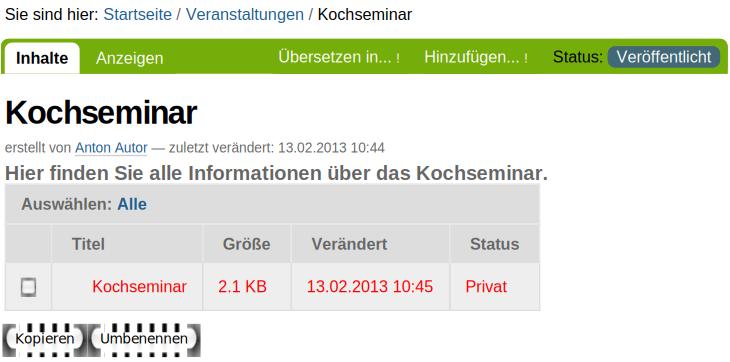
\includegraphics{folder-with-object.png}
\caption{Inhaltsansicht eines Ordners mit einem Artikel}\end{figure}
\begin{itemize}
\item {} 
Legen Sie weitere Artikel im Ordner »Kochseminar« an. Beobachten Sie
dabei stets die Ansichten »Inhalte« und »Anzeigen« des Ordners.

\end{itemize}

Sowohl in der Inhaltsansicht als auch in der von Plone erzeugten Anzeige des
Ordners kommen neue Einträge am unteren Ende hinzu. Die bestehenden Einträge
behalten dabei ihre Reihenfolge bei (siehe
Abbildung \hyperlink{fig-folder-order}{\emph{Anzeige eines Ordners mit mehreren Artikeln}}).
\hypertarget{fig-folder-order}{}\begin{figure}[htbp]
\centering

\includegraphics{folder-order.png}
\caption{Anzeige eines Ordners mit mehreren Artikeln}\end{figure}

Ändern Sie nun die Reihenfolge der Einträge. Die Inhaltsansicht des Ordners
enthält dazu in der Tabellenspalte »Reihenfolge« für jeden Artikel ein Symbol,
das aus zwei Doppelpunkten besteht.
\begin{itemize}
\item {} 
Wechseln Sie in die Inhaltsansicht des Ordners »Kochseminar«.

\item {} 
Gehen Sie mit dem Mauszeiger über die Doppelpunkte in der Tabelle. Je
nach den Einstellungen Ihres Betriebssystems verwandelt sich der Mauspfeil
dabei möglicherweise so, dass er Anfassen oder Bewegen symbolisiert.

\item {} 
Greifen Sie nun mit einem Mausklick einen Artikel, und verschieben Sie
ihn in der Liste bei gedrückter Maustaste nach oben oder unten. Wenn Sie die
Maustaste loslassen, wird der Artikel an der entsprechenden Stelle
einsortiert.

\item {} 
Wechseln Sie zwischendurch in die Anzeige des Ordners, und vergewissern
Sie sich, dass auch dort die Reihenfolge geändert wurde.

\end{itemize}

Falls Javascript an Ihrem Rechner nicht aktiviert ist, erscheinen statt der
Doppelpunkte in jeder Tabellenzeile Pfeile, mit denen Sie den jeweiligen
Artikel mit seinem Vorgänger oder Nachfolger vertauschen können.


\subsection{Ordneranzeige}

Plone kennt verschiedene Vorlagen für die Anzeige eines Ordners.
\begin{itemize}
\item {} 
Begeben Sie sich zum Ordner »Kochseminar«.

\item {} 
Öffnen Sie das Menü »Darstellung« und wählen Sie »Tabelle« aus (siehe
Abbildung \emph{fig\_ansicht}).

\end{itemize}
\hypertarget{fig-ansicht}{}
Die Anzeige des Ordners enthält jetzt anstelle der Liste eine Tabelle
mit Einträgen für jeden Artikel des Ordners.
\begin{itemize}
\item {} 
Probieren Sie nacheinander die anderen Ansichten aus. Die Albenansicht
kommt nur dann zur Geltung, wenn Sie Bilder im Ordner erstellt haben.

\end{itemize}

Plone kann anstelle von Übersichtslisten oder -tabellen auch einen Artikel aus
dem Ordner als Anzeige verwenden.
\begin{itemize}
\item {} 
Öffnen Sie das Darstellungsmenü und wählen Sie den Punkt »Artikel
aus dem Ordner...«.

\item {} 
Sie gelangen zu einem Formular, das alle im Ordner befindlichen Artikel
mit Ausnahme der Unterordner auflistet (siehe
Abbildung \hyperlink{fig-standardseite}{\emph{Auswahl eines Artikels als Ordneranzeige}}).

\end{itemize}
\hypertarget{fig-standardseite}{}\begin{figure}[htbp]
\centering

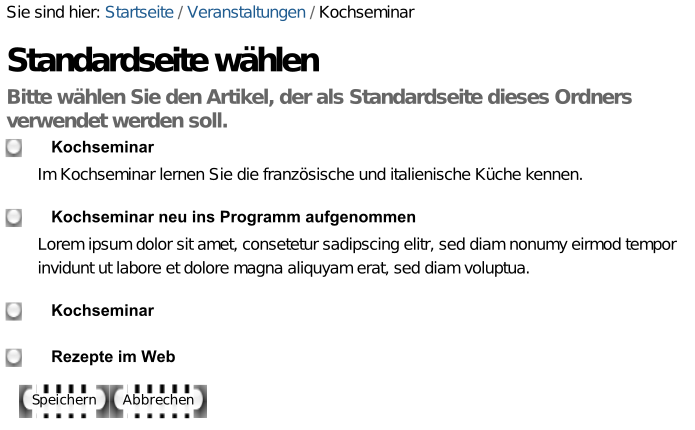
\includegraphics{standardseite.png}
\caption{Auswahl eines Artikels als Ordneranzeige}\end{figure}
\begin{itemize}
\item {} 
Kreuzen Sie den gewünschten Artikel an und speichern Sie das Formular.

\item {} 
Plone leitet Sie nun zur Anzeige des Ordners »Kochseminar« weiter. Sie
sehen dort anstelle einer Übersichtsliste oder -tabelle den gewählten
Artikel.

\item {} 
Wechseln Sie zur Inhaltsansicht. Sie sehen dort, dass der gewählte
Artikel durch Fettschrift hervorgehoben ist.

\end{itemize}


\subsection{Artikel kopieren und verschieben}

Plone erlaubt Ihnen nicht nur, Inhalte anzulegen und
zu löschen. Sie können Artikel und Ordner auch von einem Ort in der Website
an einen anderen verschieben oder kopieren.

Erzeugen Sie dazu im Ordner »Kochseminar« einen Unterordner und kopieren Sie
einen Artikel aus dem Ordner »Kochseminar« dort hinein.
\begin{itemize}
\item {} 
Legen Sie im Ordner »Kochseminar« einen Ordner an.

\item {} 
Rufen Sie anschließend im Ordner »Kochseminar« den Artikel auf, den Sie
kopieren möchten.

\item {} 
Öffnen Sie das Menü »Aktionen« und wählen Sie den Eintrag »Kopieren«

\end{itemize}

aus.
* Wechseln Sie in den Unterordner.
* Fügen Sie eine Kopie des ausgewählten Artikels dort ein, indem Sie den
\begin{quote}

Eintrag »Einfügen« im Aktionsmenü auswählen.
\end{quote}

Die Anzeige des Unterordners enthält nun einen neuen Eintrag. Vergewissern
Sie sich, dass sich am Inhalt des Ordners »Kochseminar« nichts geändert hat.

Verschieben Sie als nächstes einen Artikel aus dem Ordner »Kochseminar« in den
Unterordner. Dabei gehen Sie ähnlich vor wie beim Kopieren.
\begin{itemize}
\item {} 
Wechseln Sie in den Ordner »Kochseminar« und rufen Sie den Artikel auf,
den Sie verschieben möchten.

\item {} 
Öffnen Sie das Menü »Aktionen« und wählen Sie den Eintrag

\end{itemize}

»Ausschneiden« aus.
* Wechseln Sie in den Unterordner.
* Fügen Sie den ausgewählten Artikel dort ein, indem Sie den Eintrag
\begin{quote}

»Einfügen« im Aktionsmenü benutzen.
\end{quote}

Sie werden bemerken, dass der Artikel nicht gleich beim Ausschneiden aus dem
Ordner »Kochseminar« verschwindet. Erst beim Einfügen wird er an seinem
Ursprungsort tatsächlich gelöscht. Kontrollieren Sie nach dem Verschieben den
Inhalt des Ordners »Kochseminar«.

Sie können Artikel nicht nur einzeln mit Hilfe der Einträge im Aktionsmenü
kopieren und verschieben. In der Inhaltsansicht eines Ordners können Sie
mehrere Artikel markieren, um sie gemeinsam zu kopieren oder zu
verschieben.
\begin{itemize}
\item {} 
Wechseln Sie in die Inhaltsansicht des Ordners »Kochseminar«.

\item {} 
Markieren Sie in der Spalte ganz links einige Artikel, die Sie kopieren
möchten.

\item {} 
Betätigen Sie die Schaltfläche »Kopieren« unterhalb der
Übersichtstabelle. Achten Sie auf die Statusmeldung.

\item {} 
Wechseln Sie nun in den Unterordner.

\item {} 
Betätigen Sie die Schaltfläche »Einfügen«. Lesen Sie die Statusmeldung
und schauen Sie nach, wie sich die Übersichtsliste verändert hat.

\end{itemize}

Wenn Sie einen Ordner kopieren oder verschieben, werden alle Artikel, die sich
in dem Ordner befinden, mit dem Ordner verschoben oder kopiert.
\begin{itemize}
\item {} 
Legen Sie im Ordner »Kochseminar« einen weiteren Ordner an.

\item {} 
Wechseln Sie in die Inhaltsansicht des Ordners »Kochseminar«.

\item {} 
Markieren Sie den ersten Unterordner zum Kopieren.

\item {} 
Wechseln Sie in den neuen Unterordner.

\item {} 
Fügen Sie den markierten Ordner ein.

\end{itemize}

Der Unterordner mit seinem gesamten Inhalt befindet sich nun auch in dem
zweiten Unterordner.
\begin{itemize}
\item {} 
Vergewissern Sie sich, dass beide Ordner den gleichen Inhalt besitzen.

\end{itemize}


\subsection{Ordner löschen}

Ordner werden wie alle anderen Artikel mit der Aktion »Löschen« im
Aktionsmenü gelöscht. Beachten Sie, dass beim Löschen eines Ordners auch die
darin enthaltenen Artikel gelöscht werden.

\resetcurrentobjects
\hypertarget{--doc-tutorien/redakteur}{}

\hypertarget{sec-veroff-von-artik}{}\section{Veröffentlichung von Artikeln}

Dieses Tutorium erläutert die Arbeitsschritte, die notwendig sind, um einen
Artikel zu veröffentlichen.

Wenn Sie einen Artikel erstellen, ist er zunächst »privat«. Nur Sie selbst
haben Zugriff auf ihn. Andere Besucher der Website können den Artikel erst
einsehen, nachdem er veröffentlicht wurde. Wenn Sie Ihre Website
alleine betreiben, können Sie selbst darüber entscheiden, ob ein Artikel
veröffentlicht werden soll oder nicht. In vielen Fällen sind Sie jedoch
nicht allein für eine Website verantwortlich, sodass die Veröffentlichung von
Artikeln mit anderen Personen abgestimmt werden muss. Plone unterstützt solche
Abstimmungsprozeduren durch festgelegte Arbeitsabläufe (siehe
Abschnitt \hyperlink{sec-workflow}{\emph{Arbeitsabläufe}}).

Artikel zu verfassen, zu redigieren und zu veröffentlichen bedeutet in der
Regel eine Arbeitsteilung zwischen Personen, die unterschiedliche
Funktionen ausüben. Die einen, die wir im Folgenden als Autoren
bezeichnen, verfassen Artikel, die anderen, die Redakteure, redigieren
und veröffentlichen sie.

In Plone haben Autoren und Redakteure unterschiedliche Rechte, sodass es
empfehlenswert ist, wenn Sie dieses Tutorium zu zweit an verschiedenen
Rechnern mit verteilten Rollen durcharbeiten. Falls Sie alleine arbeiten,
müssen Sie sich während des Tutoriums ab- und mit dem Benutzernamen eines
Redakteurs wieder anmelden.


\hypertarget{sec-veroff-von-artik-1}{}\subsection{Anmelden als Autor oder Redakteur}

Wir gehen im Folgenden davon aus, dass in Ihrer Website ein Benutzer
registriert worden ist, der zusätzliche Rechte besitzt und im Ordner
»Veranstaltungen« Artikel veröffentlichen darf. Wir bezeichnen diesen Benutzer
im Folgenden als »Redakteur«. Wenn Sie die Redakteursfunktionen in diesem
Tutorium ausprobieren möchten, müssen Sie sich mit dem Benutzernamen des
Redakteurs bei Ihrer Website anmelden. Fragen Sie gegebenenfalls Ihren
Administrator nach den entsprechenden Zugangsdaten. Wenn Sie Autorenfunktionen
ausüben, können Sie sich mit Ihrem persönlichen Benutzernamen anmelden.
\hypertarget{sec-artik-zur-veroff}{}

\subsection{Artikel zur Veröffentlichung einreichen}


\hypertarget{sec-veroff-von-artik-2}{}\subsubsection{Einen einzelnen Artikel zur Veröffentlichung einreichen}
\begin{itemize}
\item {} 
Melden Sie sich auf Ihrer Website mit Ihrem Benutzernamen an.

\item {} 
Legen Sie im Ordner »Veranstaltungen« eine neue Seite an, bearbeiten Sie
Titel, Beschreibung und Haupttext und speichern Sie Ihre Eingaben.

\item {} 
Vergewissern Sie sich in der Ordnerübersicht, dass der Status des
Artikels »privat« ist und der Eintrag für den Artikel rot dargestellt
wird.

\item {} 
Reichen Sie die Seite zur Veröffentlichung ein, indem Sie zur Anzeige
des Artikels wechseln und im Statusmenü den Eintrag »Zur Veröffentlichung
einreichen« wählen (siehe
Abbildung \hyperlink{fig-auswahlmenu-zur-veroeffentlichung-einreichen}{\emph{Einen Artikel zur Veröffentlichung einreichen}}).

\end{itemize}
\hypertarget{fig-auswahlmenu-zur-veroeffentlichung-einreichen}{}\begin{figure}[htbp]
\centering

\includegraphics{zur-veroeffentlichung-einreichen.png}
\caption{Einen Artikel zur Veröffentlichung einreichen}\end{figure}
\begin{itemize}
\item {} 
Achten Sie auf die Statusmeldung und darauf, dass der Artikel in der
Ordnerübersicht nun als »zur Veröffentlichung eingereicht« geführt und in
Orange dargestellt wird.

\end{itemize}
\hypertarget{sec-veroff-von-artik-4}{}

\subsubsection{Mehrere Artikel zur Veröffentlichung einreichen}

Sie können mehrere Artikel gleichzeitig zur Veröffentlichung einreichen.
\begin{itemize}
\item {} 
Legen Sie mehrere Artikel im Ordner »Veranstaltungen« an.

\item {} 
Wechseln Sie zur Inhaltsansicht des Ordners. Ihre neuen Artikel werden
dort mit dem Status »privat« geführt und rot dargestellt.

\item {} 
Wählen Sie in der Tabelle die Artikel aus, die Sie zur Veröffentlichung
einreichen wollen.

\item {} 
Betätigen Sie die Schaltfläche »Status ändern« unterhalb der
Tabelle. Sie gelangen zu einem Formular (siehe
Abbildung \emph{fig\_formular-arbeitsablauf}),

\end{itemize}
\begin{figure}[htbp]
\centering

\includegraphics{formular-arbeitsablauf.png}
\end{figure}
\begin{itemize}
\item {} 
Geben Sie im Feld »Kommentare« eine Nachricht für Ihren Redakteur ein.

\item {} 
Setzen Sie ganz unten auf dem Formular im Abschnitt »Status verändern«
ein Häkchen bei »Zur Veröffentlichung einreichen« und speichern Sie.

\item {} 
Achten Sie auf die Statusmeldung und darauf, dass alle eingereichten
Artikel im Ordner nun den Status »zur Veröffentlichung eingereicht« tragen
und in einer anderen Farbe (Orange) dargestellt werden.

\end{itemize}

Sie erreichen das Formular auch über den Menüeintrag »Erweitert...« im
Statusmenü eines Artikels. Sie werden vor allem dann das Formular benötigen,
wenn Sie Ihrem Redakteur Kommentare hinterlassen wollen.
\hypertarget{sec-artik-redig-und}{}

\subsection{Artikel veröffentlichen und zurückweisen}

Nachdem ein Artikel zur Veröffentlichung eingereicht wurde, kommt der
Redakteur ins Spiel. Übernehmen Sie deshalb jetzt  die Rolle des Redakteurs.
\begin{itemize}
\item {} 
Melden Sie sich mit Ihrem eigenen Benutzernamen ab.

\item {} 
Melden Sie sich mit dem Benutzernamen des Redakteurs wieder an.

\end{itemize}

Nach der Anmeldung erscheint in der rechten Spalte das Portlet mit der
Revisionsliste (siehe Abbildung \hyperlink{fig-revisionsliste}{\emph{Portlet »Revisionsliste«}}).
\hypertarget{fig-revisionsliste}{}\begin{figure}[htbp]
\centering

\includegraphics{revisionsliste.png}
\caption{Portlet »Revisionsliste«}\end{figure}

Die Liste enthält Artikel, die zur Veröffentlichung eingereicht wurden und die
Sie veröffentlichen dürfen.


\hypertarget{sec-artik-redig-veroff}{}\subsubsection{Artikel veröffentlichen}
\begin{itemize}
\item {} 
Wählen Sie in der Revisionsliste einen Artikel aus.

\item {} 
Lesen und bearbeiten Sie gegebenenfalls den Artikel.

\item {} 
Veröffentlichen Sie den Artikel, indem Sie im Statusmenü den Eintrag
»Veröffentlichen« (siehe Abbildung \emph{fig\_statusmenu-veroeffentlichen})

\end{itemize}
\hypertarget{fig-statusmenu-veroeffentlichen}{}\begin{figure}[htbp]
\centering

\includegraphics{veroeffentlichen.png}
\end{figure}
\begin{itemize}
\item {} 
Achten Sie auf die Statusmeldung und darauf, dass der Artikel in der
Ordneransicht nun mit dem Status »veröffentlicht« angezeigt und in Blau
dargestellt wird.

\end{itemize}

Der veröffentlichte Artikel ist nun auch für anonyme Besucher der Website
sichtbar.
\hypertarget{sec-artik-redig-und-1}{}

\subsection{Historie des Arbeitsablaufs}

Rufen Sie den veröffentlichten Artikel auf und klappen Sie die Historie für
den Arbeitsablauf auf, indem Sie mit der Maus auf das Pluszeichen neben dem
Begriff »Historie« unterhalb des Artikels klicken (siehe
Abbildung \hyperlink{fig-historie-arbeitsablauf}{\emph{Historie des Arbeitsablaufes}}).
\hypertarget{fig-historie-arbeitsablauf}{}\begin{figure}[htbp]
\centering

\includegraphics{historie-arbeitsablauf.png}
\caption{Historie des Arbeitsablaufes}\end{figure}

Dort können Sie nachschauen, wer den Artikel wann zur Veröffentlichung
eingereicht oder veröffentlicht hat. Die Tabelle enthält eine Liste aller
Statusänderungen.


\hypertarget{sec-artik-redig-veroff-1}{}\subsubsection{Artikel zurückweisen}

Falls Sie der Meinung sind, dass ein Artikel nicht veröffentlicht werden
sollte, können Sie ihn zurückweisen.
\begin{itemize}
\item {} 
Wählen Sie in der Revisionsliste einen Artikel aus.

\item {} 
Lesen Sie den Artikel.

\item {} 
Weisen Sie den Artikel zurück, indem Sie im Statusmenü den Eintrag
»Zurückweisen« (siehe Abbildung\textasciitilde{}vref\{fig:statusmenu-veroeffentlichen\})
auswählen.

\item {} 
Achten Sie auf die Statusmeldung und darauf, dass der Artikel in der
Ordnerübersicht nun den Status »privat« trägt und in Rot dargestellt wird.

\end{itemize}

Am Status »privat« erkennt der Verfasser, dass Sie den Artikel
zurückgewiesen haben.

Da eine Zurückweisung ohne Begründung für den Verfasser zumeist unbefriedigend
ist, sollten Sie das erweiterte Formular »Arbeitsablauf« benutzen, um ihm im
Kommentarfeld eine Begründung für die Zurückweisung zu hinterlassen. Der
Verfasser des Artikels kann diesen Kommentar in der Historie nachlesen und
seinen Artikel entsprechend überarbeiten.

Falls Sie zu zweit das Tutorium durcharbeiten, wechseln Sie nun die Rollen und
gehen Sie die Arbeitsschritte dieses Abschnitts erneut durch.

\resetcurrentobjects
\hypertarget{--doc-inhaltstypen/inhaltstypen}{}

\hypertarget{sec-inhaltstypen}{}\chapter{Artikeltypen}

In diesem Kapitel werden Ihnen die Eigenschaften aller Artikeltypen
von Plone vorgestellt. Dabei gehen wir zuerst auf die Gemeinsamkeiten
ein und widmen uns danach jedem einzelnen Artikeltyp.  Tabelle
\emph{tab\_artikeltypen} gibt einen Überblick über die verfügbaren
Typen und ihre Symbole.
\hypertarget{tab-artikeltypen}{}
\begin{tabulary}{\textwidth}{|L|L|}
\hline
\textbf{
Symbol
} & \textbf{
Artikeltyp
}\\
\hline

\includegraphics{typ-seite.png}
 & 
Seite
\\

\includegraphics{typ-nachricht.png}
 & 
Nachricht
\\

\includegraphics{typ-termin.png}
 & 
Termin
\\

\includegraphics{typ-bild.png}
 & 
Bild
\\

\includegraphics{typ-datei.png}
 & 
Datei
\\

\includegraphics{typ-lesezeichen.png}
 & 
Lesezeichen
\\

\includegraphics{typ-link.png}
 & 
Link
\\

\includegraphics{typ-ordner.png}
 & 
Ordner
\\

\includegraphics{typ-kollektion.png}
 & 
Kollektion
\\
\hline
\end{tabulary}


\resetcurrentobjects
\hypertarget{--doc-inhaltstypen/gemeinsamkeiten}{}

\hypertarget{sec-inhaltstypen-gemeinsamkeiten}{}\section{Gemeinsamkeiten}

Die unterschiedlichen Artikeltypen in Plone weisen viele Gemeinsamkeiten auf.
So besitzt jeder Artikel folgende drei Ansichten:
\begin{itemize}
\item {} 
Anzeigen

\item {} 
Bearbeiten

\item {} 
Zugriff

\end{itemize}

Der Zugriff auf die einzelnen Ansichten ist Ihnen nur gestattet, wenn Sie die
jeweils dafür benötigten Rechte besitzen. Sie können mit Hilfe von Reitern
(siehe Abbildung \emph{fig\_tabs})
\hypertarget{fig-tabs}{}
zwischen den für Sie verfügbaren Ansichten eines Artikels wechseln.

Anzeige und Bearbeitungsansicht sind in ihren Grundzügen für alle Artikel
gleich. Sie werden direkt im Anschluss erläutert, die Ansicht »Zugriff« in
Abschnitt \hyperlink{sec-zugriffsrechte-ansicht}{\emph{Artikelansicht »Freigabe«}}.


\hypertarget{sec-gemeinsamkeiten-anzeige}{}\subsection{Anzeige}

Die Anzeigeansicht stellt einen Artikel so dar, wie ihn Besucher der Website sehen
sollen. Ihr Aussehen und die enthaltenen Informationen hängen vom Artikeltyp
ab. Beispielsweise werden für eine Seite hauptsächlich Titel, Beschreibung und
Haupttext angezeigt, während in einem Termin weitergehende Informationen wie
der Zeitpunkt und Ort des Ereignisses erscheinen. Die einzelnen
Artikeltypen und die Eigenheiten ihrer Anzeige werden in diesem Kapitel ab
Seite \hyperlink{sec-dokument}{\emph{Seite}} genauer beschrieben.

Die Anzeigeansichten aller Artikel haben jedoch einige Gemeinsamkeiten (siehe
Abbildung \hyperlink{fig-gemeinsamkeiten-anzeige}{\emph{Aufbau der Anzeige eines Artikels Aufbau der Anzeige eines Artikels: Titel\textasciitilde{}(1), Verfasserzeile\textasciitilde{}(2), Beschreibung\textasciitilde{}(3), Artikelaktionen\textasciitilde{}(4), Historie\textasciitilde{}(5) und Vor- und Zurückblättern\textasciitilde{}(6)}}):
\hypertarget{fig-gemeinsamkeiten-anzeige}{}\begin{figure}[htbp]
\centering

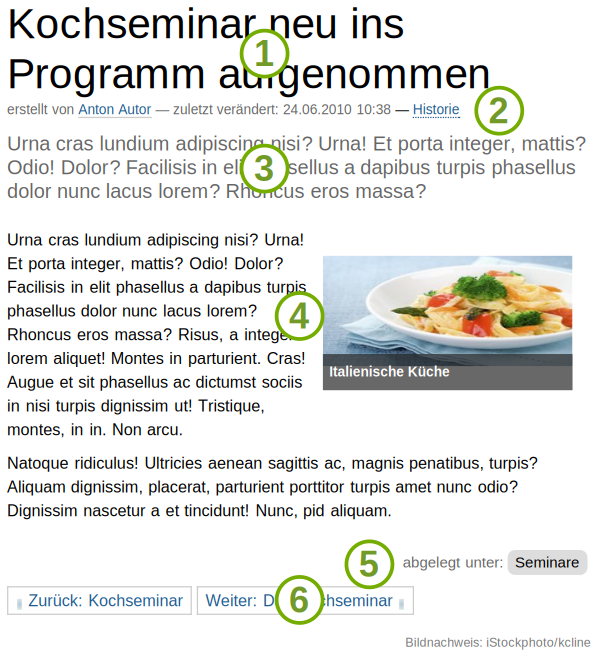
\includegraphics{gemeinsamkeiten-anzeige.png}
\caption{Aufbau der Anzeige eines Artikels Aufbau der Anzeige eines Artikels: Titel\textasciitilde{}(1), Verfasserzeile\textasciitilde{}(2), Beschreibung\textasciitilde{}(3), Artikelaktionen\textasciitilde{}(4), Historie\textasciitilde{}(5) und Vor- und Zurückblättern\textasciitilde{}(6)}\end{figure}
\begin{itemize}
\item {} 
Titel

\item {} 
Verfasserzeile

\item {} 
Beschreibung

\item {} 
Artikelaktionen

\item {} 
Historie (nur für angemeldete Benutzer sichtbar)

\item {} 
Vor- und Zurückblättern (je nach Einstellungen des Ordners)

\end{itemize}

Die Verfasserzeile eines Artikels gibt an, wer den Artikel erstellt hat und
wann er zuletzt geändert wurde. Der Name des Erstellers ist ein Verweis zu
seinem Profil. Beachten Sie, dass die Verfasserzeile nicht angibt, wer die
letzte Änderung gemacht hat. Die Verfasserzeile wird je nach Konfiguration der
Website möglicherweise nur angemeldeten Benutzern angezeigt.
\hypertarget{sec-anzeige-waehlen}{}
Manche Artikel wie beispielsweise Ordner und Kollektionen können ihren
Inhalt auf mehr als eine Art und Weise darstellen. In solchen Fällen finden
Sie in dem grünen Rahmen um die Anzeige ein Ausklappmenü mit dem
Titel »Darstellung«, aus dem Sie eine der möglichen Darstellungen auswählen
können (siehe Abbildung \emph{fig:anzeige-waehlen}).
\hypertarget{fig-anzeige-waehlen}{}\begin{figure}[htbp]
\centering

\includegraphics{anzeige-waehlen.png}
\caption{Darstellung eines Ordners auswählen}\end{figure}
\hypertarget{sec-bearbeiten}{}

\subsection{Bearbeiten}

Wenn Sie einen Artikel verändern möchten, gibt es zwei Möglichkeiten: die
Sofortbearbeitung und die Bearbeitungsansicht.

Sofortbearbeitung bedeutet, dass Sie den Titel, die Beschreibung oder den
Haupttext in der Anzeige des Artikels mit der Maus anklicken können und
daraufhin ein Bearbeitungsfeld für das Element erscheint (siehe
Abbildung \hyperlink{fig-sofortbearbeitung}{\emph{Die Sofortbearbeitung einer Seite}}).
\hypertarget{fig-sofortbearbeitung}{}\begin{figure}[htbp]
\centering

\includegraphics{titel-bearbeiten-ajax.png}
\caption{Die Sofortbearbeitung einer Seite}\end{figure}

Der Mauszeiger verwandelt sich dabei in einen Cursor, und unterhalb des
angewählten Elements erscheinen Schaltflächen zum Speichern und Abbrechen der
Bearbeitung. Für den Haupttext öffnet sich der visuelle Editor Kupu.

Die Sofortbearbeitung steht nur zur Verfügung, wenn Sie Javascript
eingeschaltet haben, und ist nur für bestimmte
Artikelelemente möglich. Sie können diese Elemente daran erkennen, dass um sie
herum ein Bearbeitungsrahmen erscheint, sobald Sie mit der Maus darüberfahren.

Jeder Artikel besitzt darüber hinaus eine Bearbeitungsansicht, in der man alle
seine Merkmale verändern kann. Ob Sie einen Artikel überhaupt modifizieren
dürfen, hängt von Ihren Rechten und vom Status des Artikels ab (siehe
Abschnitte \hyperlink{sec-benutzer-rollen}{\emph{Funktionen}} und \emph{sec:workflow}).

Es handelt sich bei der Bearbeitungsansicht um ein gegliedertes
Formular, das aus folgenden Teilen besteht:
\begin{itemize}
\item {} 
Standard

\item {} 
Kategorisierung

\item {} 
Datum

\item {} 
Urheber

\item {} 
Einstellungen

\end{itemize}

Sie erreichen die einzelnen Teilformulare über die Navigationsleiste unterhalb
der Seitenüberschrift (siehe Abbildung \hyperlink{fig-bearbeiten-teilformulare}{\emph{Auswahl eines Teilformulars der Bearbeitungsansicht}}).
\hypertarget{fig-bearbeiten-teilformulare}{}\begin{figure}[htbp]
\centering

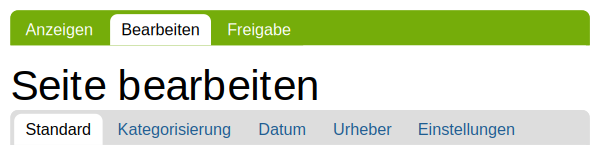
\includegraphics{bearbeiten-teilformulare.png}
\caption{Auswahl eines Teilformulars der Bearbeitungsansicht}\end{figure}

Zunächst ist das Standardformular aktiv. Falls Sie
Javascript in Ihrem Browser ausgeschaltet haben, werden alle Teilformulare
gleichzeitig untereinander angezeigt.

Unter jedem Teilformular finden Sie ein Eingabefeld für eine Änderungsnotiz.


\hypertarget{sec-teilf-stand}{}\subsubsection{Teilformular »Standard«}

Im Teilformular »Standard« (siehe Abbildung \hyperlink{fig-bearbeiten}{\emph{Bearbeitungsansicht einer Seite}})
\hypertarget{fig-bearbeiten}{}\begin{figure}[htbp]
\centering

\includegraphics{seite-bearbeiten-standard.png}
\caption{Bearbeitungsansicht einer Seite}\end{figure}

werden diejenigen Informationen eingetragen, die im Allgemeinen für die
Öffentlichkeit bestimmt sind und den wesentlichen Inhalt des Artikels
ausmachen:
\begin{itemize}
\item {} 
Titel

\item {} 
Beschreibung

\item {} 
sonstige Inhalte (beispielsweise der Haupttext)

\end{itemize}

Ob Sie darüber hinaus ein Eingabefeld für den Kurznamen sehen, hängt von den
Einstellungen für Ihre Website und von Ihren persönlichen Einstellungen ab. Mehr
zu Kurznamen erfahren Sie in Abschnitt \hyperlink{sec-kurzname}{\emph{Kurznamen und Umbenennen}}.

Wählen Sie für jeden Artikel einen kurzen, jedoch aussagekräftigen Titel, der
sich direkt auf den Inhalt bezieht. Da Plone die
Titel beispielsweise für die Navigation benutzt, wird Ihre Website
dadurch übersichtlicher und ihr Aufbau besser verständlich. Außerdem tragen
gut gewählte Titel dazu bei, dass Ihre Seiten von Suchmaschinen im Internet
höher bewertet und damit von interessierten Besuchern leichter gefunden
werden.

Die Beschreibung sollte aus einem kurzen Text bestehen, der den Inhalt
umreißt oder als Einleitung dient. Sie erscheint zum einen als
Zusammenfassung in der Artikelanzeige, zum anderen in Listen wie der von Plone
erzeugten Ordnerübersicht.

Bei allen Artikeltypen außer bei Ordnern und Kollektionen dient das Teilformular
»Standard« dazu, den Inhalt des Artikels zu verändern. Welche Möglichkeiten
Sie dabei haben, hängt stark vom jeweiligen Typ ab und wird später im
Einzelnen erläutert. Ordner und Kollektionen hingegen besitzen keinen eigenen
redaktionellen Inhalt.
\hypertarget{sec-teilf-kateg}{}

\subsubsection{Teilformular »Kategorisierung«}

Im Teilformular »Kategorisierung« (siehe
Abbildung \emph{fig\_seite-bearbeiten-kategorisierung})
\begin{figure}[htbp]
\centering

\includegraphics{seite-bearbeiten-kategorisierung.png}
\caption{Das Teilformular »Kategorisierung«}\end{figure}

können Sie Artikel kategorisieren. Dabei versehen Sie jeden Artikel mit
Informationen wie der Sprache, in der er verfasst ist, oder einer inhaltlichen
Kategorie, in die er gehört. Solche Informationen werden als Metadaten
bezeichnet (siehe Abschnitt \hyperlink{sec-exkurs-metadaten}{\emph{Metadaten und der Dublin-Core-Standard}}). Um weitere
Metadaten geht es in den Teilformularen »Datum« und »Urheber«.
\hypertarget{sec-teilf-kateg-1}{}
Kategorien
\begin{quote}

Kategorien in Plone sind Stichwörter, mit denen ein Artikel verschlagwortet
wird. Sie helfen beim Auffinden oder Gruppieren inhaltlich verwandter
Artikel.

Wenn Ihre Website schon länger aktiv ist, kennt sie bereits eine Reihe von
Stichwörtern und bietet sie Ihnen in diesem Feld zur Auswahl an. Redakteure
haben die Möglichkeit, neue Stichwörter zur Auswahl hinzuzufügen.
\end{quote}
\hypertarget{sec-teilf-kateg-2}{}
Verweise
\begin{quote}

Verweise dienen dazu, den Leser eines Artikels auf bestimmte andere Artikel
hinzuweisen, die mit dem angezeigten in Verbindung stehen. Sie werden in der
Anzeige eines Artikels unterhalb des Inhalts angezeigt und besonders
hervorgehoben.

Das Teilformular »Kategorisierung« enthält eine Liste der eingetragenen
Verweise. Darunter befindet sich eine Schaltfläche, mit der man neue Verweise
hinzufügen kann. Wenn man sie betätigt, öffnet sich ein Fenster mit der
Artikelliste des aktuellen Ordners, einem Verzeichnispfad und einem Suchfeld
(siehe Abbildung \emph{fig\_verweise-artikel-suchen}).
\end{quote}
\hypertarget{fig-verweise-artikel-suchen}{}\begin{figure}[htbp]
\centering

\includegraphics{verweise-artikel-suchen.png}
\end{figure}

Ort{]}
\begin{quote}

Sie können hier den Artikel in Bezug zu einem geografischen Ort setzen. Einige
Erweiterungen für Plone können diese Information auswerten, indem
sie Orte beispielsweise auf einer Weltkarte markieren.
\end{quote}

Sprache
\begin{quote}

In diesem Menü können Sie die Sprache auswählen, in der der Artikel verfasst
ist. Die voreingestellte Sprache hängt von Ihrer Website ab.
\end{quote}
\hypertarget{sec-teilformular-datum}{}

\subsubsection{Teilformular »Datum«}

Das Teilformular »Datum« dient dazu, die Anzeigedauer des Artikels
zu beschränken (siehe Abbildung \emph{fig\_seite-bearbeiten-datum}).
\begin{figure}[htbp]
\centering

\includegraphics{seite-bearbeiten-datum.png}
\caption{Das Teilformular »Datum«}\end{figure}

Freigabedatum
\begin{quote}

Mit dem Freigabedatum bestimmen Sie, wann ein Artikel Besuchern zur Ansicht
freigegeben wird. Selbst wenn ein Artikel die interne, redaktionelle Prüfung
durchlaufen hat und sich im Status »veröffentlicht« befindet, wird er erst
nach dem Freigabedatum wirklich sichtbar.
\end{quote}

Ablaufdatum
\begin{quote}

Ist ein Ablaufdatum eingestellt, wird der Artikel ausgeblendet, sobald es
erreicht ist.

Beide Einträge zusammen bilden die Angabe »Verfügbarkeitszeitraum« des
Dublin-Core-Standards (siehe dazu Abschnitt \hyperlink{sec-exkurs-metadaten}{\emph{Metadaten und der Dublin-Core-Standard}}).

Sie können das Datum bei beiden Feldern mit Hilfe des aufklappbaren Kalenders
eingeben, den Sie über das Kalendersymbol zwischen Datum und Uhrzeit
erreichen. Um ein früher eingegebenes Datum zu löschen, wählen Sie für das
Jahr »- - - -« aus.
\end{quote}
\hypertarget{sec-teilformular-urheber}{}

\subsubsection{Teilformular »Urheber«}

Im Teilformular »Urheber« (siehe
Abbildung \emph{fig\_seite-bearbeiten-urheber})
\hypertarget{fig-seite-bearbeiten-urheber}{}\begin{figure}[htbp]
\centering

\includegraphics{seite-bearbeiten-urheber.png}
\end{figure}

Das Teilformular »Urheber«

können Sie die Personen aufführen, die an der Erstellung des Artikels
mitgewirkt haben, und Angaben zu den Urheberrechten machen.

Ersteller
\begin{quote}

Tragen Sie einen oder mehrere Benutzernamen ein. Um mehrere
Personen aufzuführen, schreiben Sie jeden Namen in eine eigene Zeile des
Feldes.
\end{quote}

Beitragende
\begin{quote}

Hier tragen Sie die realen Namen weiterer Personen ein, die
einen Beitrag geleistet haben. Verwenden Sie wieder eine eigene Zeile für
jeden Namen. Wie Sie Ersteller und Beitragende voneinander abgrenzen, ist
keine technische, sondern eine redaktionelle Frage. Die Ersteller sind
gemeinhin diejenigen Personen, die an der Erstellung des Artikels auf der
Website beteiligt waren. Beitragende haben in der Regel Informationen
beigesteuert, den Artikel auf der Website aber nicht selbst bearbeitet. Sie
müssen nicht einmal auf der Website registriert sein.
\end{quote}

Urheberrechte
\begin{quote}

In diesem Formularfeld können Sie beispielsweise eine
Creative-Commons-Lizenz angeben oder sich alle Rechte
vorbehalten. Eventuell ist dieses Feld bereits von Ihrem
Systemverwalter ausgefüllt worden. Hier ist auch der geeignete Ort,
um auf Rechte Dritter aufmerksam zu machen.
\end{quote}
\hypertarget{sec-teilf-einst}{}

\subsubsection{Teilformular »Einstellungen«}

Welche Einstellungen Sie in diesem Teilformular vornehmen können, hängt vom
Typ des betroffenen Artikels ab. Die folgenden zwei Einstellungen sind allen
Artikeltypen gemeinsam. Abbildung \hyperlink{fig-seite-bearbeiten-einstellungen}{\emph{Das Teilformular »Einstellungen«}}
\hypertarget{fig-seite-bearbeiten-einstellungen}{}\begin{figure}[htbp]
\centering

\includegraphics{seite-bearbeiten-einstellungen.png}
\caption{Das Teilformular »Einstellungen«}\end{figure}

zeigt das Teilformular »Einstellungen« für eine Seite.

Kommentare erlauben
\begin{quote}

Ihre Website kann so konfiguriert sein, dass für
manche Artikeltypen Kommentare im Allgemeinen erlaubt sind. Bei Artikeln
dieser Typen ist hier das Häkchen bereits gesetzt. Sie können ungeachtet
dieser Einstellungen das Kommentieren eines einzelnen Artikels erlauben oder
verbieten, indem Sie hier ein Häkchen setzen oder entfernen.
\end{quote}

Von Navigation ausschließen
\begin{quote}

Per Voreinstellung tauchen bestimmte
Artikeltypen im Navigationsportlet oder der Navigationsleiste auf. Hier
können Sie einzelne Artikel von der Anzeige in der Navigation ausschließen.
\end{quote}

Die übrigen Einstellungsmöglichkeiten der einzelnen Artikeltypen werden in den
nachfolgenden Abschnitten erläutert.


\paragraph{Bearbeitungsansicht gesperrt}

Falls Sie einen Artikel aufrufen, der in diesem Moment bereits von einem
anderen Benutzer bearbeitet wird, erhalten Sie einen entsprechenden
Warnhinweis (siehe Abbildung \emph{fig\_locking}).
\hypertarget{fig-locking}{}\begin{figure}[htbp]
\centering

\includegraphics{locking.png}
\end{figure}

Warnmeldung beim Zugriff auf gesperrten Artikel

Die Bearbeitungsansicht ist
für Sie gesperrt, das heißt der Reiter »Bearbeiten« fehlt. Wenn Sie sicher
sind, dass der genannte Benutzer den Artikel nicht mehr bearbeitet, können Sie
die Sperrung aufheben, indem Sie die Schaltfläche »Entsperren« betätigen.
\hypertarget{sec-exkurs-metadaten}{}

\subsubsection{Metadaten und der Dublin-Core-Standard}

Wenn Sie schon einmal in einer Bibliothek nach einem bestimmten Buch gesucht
haben, sind sie bereits mit Metadaten konfrontiert worden. So haben Sie
vielleicht im Stichwortkatalog nach Büchern gesucht, die ein bestimmtes Thema
behandeln. Plone besitzt etwas Ähnliches für den Inhalt einer Website.

Metadaten sind beschreibende Angaben zu einem Artikel.  Mit ihrer Hilfe kann
ein Leser den Artikel inhaltlich einordnen und abschätzen, ob er für ihn von
Interesse ist, ohne ihn erst vollständig zu lesen.  Zudem können Metadaten
auch maschinell auf einfache Weise ausgewertet werden.

Die Artikel in einer Plone-Website besitzen eine Anzahl von Metadaten, von
denen einige auch öffentlich angezeigt werden. Dazu
zählen beispielsweise der Titel und die Kategorien, in die ein Artikel
einsortiert wurde. So können Suchmaschinen Ihre Inhalte besser katalogisieren
und wiederfinden.

Damit Metadaten verschiedener Artikel vergleichbar sind, wurde der
Dublin-Core-Standard entwickelt (siehe
url\{\href{http://dublincore.org/documents/dcmi-terms/}{http://dublincore.org/documents/dcmi-terms/}\}). Dieser Standard legt eine
Anzahl von Angaben fest, die in den Metadaten für einen Artikel enthalten sein
sollten. Er wird nicht nur im Content-Management angewandt, sondern
erleichtert beispielsweise Bibliotheken den Austausch von Informationen über
ihre Datenbestände.

Metadaten nach Dublin-Core-Standard umfassen derzeit 15\textasciitilde{}Basisangaben und
eine größere Zahl zusätzlicher, feiner unterteilter Felder.
Tabelle \emph{tab\_dublincore} fasst zusammen, welche davon in Plone verfügbar sind.
\hypertarget{tab-dublincore}{}
Von Plone verwendete Metadaten nach Dublin-Core:
\begin{itemize}
\item {} 
Titel

\item {} 
Ersteller

\item {} 
Herausgeber

\item {} 
Beitragende

\item {} 
Kategorien

\item {} 
Inhaltliche Beschreibung

\item {} 
Sprache

\item {} 
Erstellungsdatum

\item {} 
Änderungsdatum

\item {} 
Verfügbarkeitszeitraum

\item {} 
Artikeltyp

\item {} 
Format

\item {} 
Ressourcen-Identifikation

\item {} 
Urheberrecht

\end{itemize}

Die Metadaten von Artikeln kommen in Plone an vielen Stellen zum Einsatz.


\hypertarget{sec-nutz-von-metad-1}{}\paragraph{Erweiterte Suche}

Besonders nützlich sind Metadaten für die erweiterte Suche
(siehe Abbildung \hyperlink{fig-erweiterte-suche}{\emph{Erweiterte Suche}}).
\hypertarget{fig-erweiterte-suche}{}\begin{figure}[htbp]
\centering

\includegraphics[width=1.000\linewidth]{erweiterte-suche.png}
\caption{Erweiterte Suche}\end{figure}

Sie erreichen sie, indem Sie die Schnellsuche benutzen und dann dem Verweis
»Erweiterte Suche« folgen.

Einige der erweiterten Suchkriterien sind dazu da, Artikel anhand ihrer
Metadaten zu finden. So kann man beispielsweise Stichwörter angeben oder das
Beschreibungsfeld von Artikeln nach Begriffen durchsuchen. Außerdem kann man
die Suche auf Artikel beschränken, die in einer bestimmten Zeitspanne
hinzugefügt oder von einem bestimmten Autor verfasst wurden.
\hypertarget{sec-nutz-von-metad-3}{}

\paragraph{Portlets}

In vielen Portlets spielen Metadaten eine Rolle. So listet das Portlet
»Aktuelle Änderungen« die fünf Artikel auf, die zuletzt verändert
wurden (siehe Abbildung :ref:fig\_portlet-recent).
\hypertarget{fig-portlet-recent}{}\begin{figure}[htbp]
\centering

\includegraphics{portlet-recent.png}
\caption{Portlet »Aktuelle Änderungen«}\end{figure}

Hier wird der Zeitstempel »zuletzt verändert« benutzt, den Plone
automatisch immer dann aktualisiert, wenn ein Artikel verändert und
gespeichert wird.

Ähnlich funktionieren die Portlets für Nachrichten und Termine, in denen die
fünf neuesten Nachrichten und Termine aufgelistet werden. Hier verwendet Plone
einen Zeitstempel, der einmalig beim Erzeugen eines Artikels gesetzt wird: das
Erstellungsdatum.
\hypertarget{sec-nutz-von-metad-4}{}

\paragraph{Kollektionen}

Kollektionen listen Artikel aus der gesamten Website auf, die bestimmte
Kriterien erfüllen. Wie bei der erweiterten Suche gibt es dafür ganz
unterschiedliche Kriterien, die sich auch häufig auf Metadaten beziehen.
Mehr über Kollektionen erfahren Sie in Abschnitt \hyperlink{sec-thema}{\emph{Kollektion}}.


\paragraph{Maschinenlesbare Metadaten im HTML-Quellcode}

Metadaten nach dem Dublin-Core-Schema können auch maschinenlesbar in den
HTML-Quellcode Ihrer Webseiten eingebunden werden. Dadurch können
Suchmaschinen Ihre Seiten effizienter einordnen. Diese Funktion ist
in Plone zunächst nicht aktiviert. Fragen Sie Ihren Systemadministrator,
wenn Sie Dublin-Core-Metadaten in Ihre Webseiten einbinden möchten.

\resetcurrentobjects
\hypertarget{--doc-inhaltstypen/dokument}{}

\hypertarget{sec-dokument}{}\section{Seite}

Eine Seite ist ein Text, dessen Struktur und Darstellung Sie frei bestimmen
können. Dazu stehen Ihnen unter anderem Überschriften, Textformatierungen,
Verweise, Bilder und Grafiken zur Verfügung (siehe
Abbildung \hyperlink{fig-dokument}{\emph{Anzeige einer Seite}}).
\hypertarget{fig-dokument}{}\begin{figure}[htbp]
\centering

\includegraphics{dokument.png}
\caption{Anzeige einer Seite}\end{figure}

Wenn Sie Ihren Text eingeben, verwenden Sie in der Regel den visuellen Editor
Kupu (siehe Abschnitt \hyperlink{sec-kupu}{\emph{Der Editor Kupu}}). Er macht es Ihnen sehr einfach, die
Struktur Ihres Textes auszuzeichnen, und zeigt den Text bereits so an, wie er
später in der Seitenanzeige aussehen wird. Daneben bietet Ihnen Kupu die
wichtigsten Funktionen üblicher Textverarbeitungsprogramme, um Ihren Text zu
formatieren.

Falls Sie Kupu nicht benutzen, finden Sie stattdessen ein
einfaches Formularfeld vor, in das sie unformatierten Text, HTML-Code oder
Text in einer vereinfachten Textauszeichnungssprache wie Restructured Text,
Markdown oder Textile eingeben können. Plone verwandelt alle Eingaben in
gültiges HTML.

Haben Sie einen Text mit einem Textverarbeitungsprogramm geschrieben und
wollen ihn in dessen Dateiformat veröffentlichen, sollten Sie dafür den
Artikeltyp »Datei« benutzen.


\subsection{Präsentationsmodus}

Wenn Sie eine Seite bearbeiten, können Sie im Teilformular »Einstellungen«
den Präsentationsmodus aktivieren. Dann erscheint in der Anzeige der Seite
ein Verweis unterhalb der Überschrift: »Als Präsentation darstellen...«. Im
Präsentationsmodus wird der Inhalt der Seite auf mehrere nacheinander
anzuzeigende Bildschirmseiten verteilt, die sich gestalterisch
beispielsweise für die Projektion in einem Vortragsraum eignen (siehe
Abbildung \emph{fig\_seite-praesentationsmodus}).
\hypertarget{fig-seite-praesentationsmodus}{}\begin{figure}[htbp]
\centering

\includegraphics{praesentationsmodus.png}
\end{figure}

Eine Seite im Präsentationsmodus

Beachten Sie, dass auf den Präsentationsseiten lediglich Überschriften und
Listen erscheinen; Fließtext wird ausgeblendet.

Technisch ist die Präsentation nichts anderes als die Anzeigeansicht mit
Darstellungsanweisungen, denen das S5-System zugrunde liegt. Mehr über S5
erfahren Sie unter url\{\href{http://yatil.de/s5/}{http://yatil.de/s5/}\} oder
url\{\href{http://meyerweb.com/eric/tools/s5/}{http://meyerweb.com/eric/tools/s5/}\}.


\subsection{Inhaltsverzeichnis}

Bei längeren Texten mit vielen Zwischenüberschriften kann Plone an den
Anfang der Seite ein Inhaltsverzeichnis mit Verweisen zu den einzelnen
Abschnitten setzen (siehe Abbildung \hyperlink{fig-seite-inhaltsverzeichnis}{\emph{Automatisch erzeugtes Inhaltsverzeichnis}}).
\hypertarget{fig-seite-inhaltsverzeichnis}{}\begin{figure}[htbp]
\centering

\includegraphics{seite-inhaltsverzeichnis.png}
\caption{Automatisch erzeugtes Inhaltsverzeichnis}\end{figure}

Sie müssen das Inhaltsverzeichnis in den Einstellungen der Seite aktivieren.

\resetcurrentobjects
\hypertarget{--doc-inhaltstypen/nachricht}{}

\hypertarget{sec-nachricht}{}\section{Nachricht}

Nachrichten sind ähnlich aufgebaut wie Seiten. Sie sollen vom Leser innerhalb
der Website als aktuelle Mitteilungen wahrgenommen werden:
\begin{itemize}
\item {} 
Der Eintrag »Nachrichten« in der Hauptnavigation führt zu einer
Übersicht aller veröffentlichten Nachrichten.

\item {} 
Das Nachrichtenportlet (siehe Abbildung \hyperlink{fig-portlet-news}{\emph{Nachrichtenportlet}})
zeigt Ihnen die Titel der fünf neuesten Nachrichten an.

\end{itemize}
\hypertarget{fig-portlet-news}{}\begin{figure}[htbp]
\centering

\includegraphics{portlet-news.png}
\caption{Nachrichtenportlet}\end{figure}

Beide Listen enthalten nur Nachrichten im Revisionsstatus »veröffentlicht«.
Sie sind nach dem Erstellungsdatum sortiert und beginnen mit der neuesten
Nachricht. Das Portlet zeigt zu jeder Nachricht das Änderungsdatum an.

Im Unterschied zu Seiten gehört zum Inhalt einer Nachricht außer dem
Text ein Titelbild. Es erscheint sowohl in der Anzeige der Nachricht
(siehe Abbildung \hyperlink{fig-nachricht}{\emph{Anzeige einer Nachricht}}) als auch in der
Nachrichtenübersicht der Website neben dem Beschreibungstext des
Artikels. Das Titelbild hat nichts mit den Bildern zu tun, die Sie
beispielsweise mit Kupu in den Nachrichtentext einbetten können.
\hypertarget{fig-nachricht}{}\begin{figure}[htbp]
\centering

\includegraphics{nachricht.png}
\caption{Anzeige einer Nachricht}\end{figure}

In der Bearbeitungsansicht einer Nachricht können Sie das Titelbild auf Ihrem
Rechner auswählen und hochladen (siehe
Abbildung \hyperlink{fig-nachricht-bild-einfuegen}{\emph{Ein Titelbild in eine Nachricht einfügen}}).
\hypertarget{fig-nachricht-bild-einfuegen}{}\begin{figure}[htbp]
\centering

\includegraphics{nachricht-bild-einfuegen.png}
\caption{Ein Titelbild in eine Nachricht einfügen}\end{figure}

In einem Feld darunter sollten Sie einen Bildtitel eingeben. Haben Sie für
dieselbe Nachricht bereits früher ein Bild hochgeladen, so wird es
angezeigt. Sie können es beibehalten, löschen oder durch ein anderes Bild
ersetzen. Plone verkleinert große Bilder so, dass sie sich für die Verwendung
im Web eignen.

\resetcurrentobjects
\hypertarget{--doc-inhaltstypen/termin}{}

\hypertarget{sec-termin}{}\section{Termin}

Artikel vom Typ Termin kündigen zeitlich festgelegte Ereignisse an,
beispielsweise Veranstaltungen. Eine solche Ankündigung enthält für Termine
typische Informationen wie Anfang und Ende des Ereignisses, einen Ort und
einen Ansprechpartner. Diese Termininformationen haben eigene Eingabefelder im
Bearbeitungsformular und werden strukturiert gespeichert, damit Plone sie
direkt benutzen kann.

Wie die Seite verfügt auch der Termin über Felder für Titel, Beschreibung und
Haupttext. Letzterer wird im Termin jedoch als Terminankündigung bezeichnet.
Dort haben Sie die Möglichkeit, mit dem Texteditor Kupu einen formatierten Text
mit Zwischenüberschriften, Bildern, Tabellen und anderen Elementen einzugeben.
\hypertarget{fig-termin}{}\begin{figure}[htbp]
\centering

\includegraphics{termin.png}
\caption{Anzeige eines Termins}\end{figure}

Zu den strukturierten Angaben eines Termins mit eigenen Eingabefeldern in der
Bearbeitungsansicht gehören:

Terminort (Wo)
\begin{quote}

Ort des Ereignisses, Treffpunkt
\end{quote}

Terminanfang, Terminende (Wann)
\begin{quote}

Zeitraum, in dem das Ereignis stattfindet
\end{quote}

Terminankündigung
\begin{quote}

Ankündigung einer Veranstaltung, Einladung zu einem Treffen
\end{quote}

Teilnehmer
\begin{quote}

Liste der erwarteten Teilnehmer
\end{quote}

Terminart (Was)
\begin{quote}

Wählen Sie eine oder mehrere Kategorien aus, oder legen
Sie neue an.
\end{quote}

URL
\begin{quote}

Internetadresse mit weiteren Informationen
\end{quote}

Kontaktname
\begin{quote}

Name des Ansprechpartners bei Fragen zum Ereignis
\end{quote}

Kontaktadresse
\begin{quote}

E-Mail-Adresse des Ansprechpartners
\end{quote}

Kontakttelefon
\begin{quote}

Rufnummer des Ansprechpartners
\end{quote}

Dabei sind nur Terminanfang und Terminende Pflichtfelder.

Plone wertet die zusätzlichen Felder gezielt aus, um eine einfache
Terminverwaltung anbieten zu können:
\begin{itemize}
\item {} 
Strukturierte Angaben werden in der Anzeige jedes Termins in einer
Tabelle dargestellt (siehe Abbildung \hyperlink{fig-termin}{\emph{Anzeige eines Termins}}).

\item {} 
Über den Eintrag »Termine« in der Hauptnavigation erreichen Sie eine
Übersicht künftiger und vergangener Termine.

\item {} 
Das Terminportlet (siehe Abbildung \hyperlink{fig-portlet-events}{\emph{Terminportlet}})
unterrichtet Sie über die jeweils fünf nächsten Termine. Zu
jedem Termin sehen Sie Titel, Ort und Anfangsdatum. Wenn Sie den Mauszeiger
über den Titel halten, wird der Anfang des Beschreibungstextes angezeigt.

\item {} 
Plone trägt Termine ins Kalenderportlet ein (siehe
Abbildung \hyperlink{fig-portlet-calendar}{\emph{Kalenderportlet}}).
Der Titel des Portlets gibt an, welcher Monat gerade angezeigt wird. Er
enthält außerdem Verweise auf den jeweils vorherigen und nächsten Monat;
zunächst zeigt der Kalender den aktuellen Monat an. Der aktuelle Tag ist mit
einem orangefarbenen Rahmen markiert.

Ist für einen Tag mindestens ein Termin bekannt, so wird er im Kalender
hervorgehoben und dient als Verweis zu einer Liste aller Termine des
betreffenden Tages. Wenn Sie den Mauszeiger über einen solchen Tag halten,
sehen Sie seine Termine mit Anfangszeit, Endzeit und Titel.

\item {} 
In der Anzeige und bei den Artikelaktionen eines Termins können Sie
Kalenderdateien im iCal- und vCal-Format (iCalendar/vCalendar)
herunterladen, um den Termin in das Kalenderprogramm auf Ihrem lokalen
Rechner zu übernehmen.

\end{itemize}
\hypertarget{fig-portlet-events}{}\begin{figure}[htbp]
\centering

\includegraphics{portlet-events.png}
\caption{Terminportlet}\end{figure}
\hypertarget{fig-portlet-calendar}{}\begin{figure}[htbp]
\centering

\includegraphics{portlet-calendar.png}
\caption{Kalenderportlet}\end{figure}

Die Terminübersicht und das Kalenderportlet berücksichtigen per Voreinstellung
nur Termine im Revisionsstatus »veröffentlicht«.

Vergessen Sie bei der Eingabe der Adresse für weitere Informationen zum Termin
nicht, dass eine Webadresse mit \code{http://} beginnen muss. Wenn Sie
diesen Teil der Adresse weglassen, erhalten Sie eine Fehlermeldung. Plone
speichert nur Adressen mit vollständigem URL-Schema, beispielsweise
\code{http}, \code{https} oder \code{ftp}.

Plone achtet darauf, dass Ihre Datumsangaben für Anfang und Ende des Termins
gültig sind und der Anfangszeitpunkt nicht nach dem Ende liegt.

\resetcurrentobjects
\hypertarget{--doc-inhaltstypen/bild}{}

\hypertarget{sec-bild}{}\section{Bild}

Der Artikeltyp »Bild« dient dazu, einzelne Bilder in einer Website zu
verwalten. Sie können in Ordner einsortiert werden und besitzen Eigenschaften und Metadaten.
Will man in einer Seite eine Illustration verwenden, so muss sie als Artikel
vom Typ »Bild« in der Website liegen. Als einzige Ausnahme werden die
Titelbilder von Nachrichten in der Bearbeitungsansicht der Nachricht direkt
hochgeladen. Sie können nicht in anderen Artikeln verwendet werden.

Die Anzeige eines Bildes besteht aus dem Bild zusammen mit dem
Titel, der Beschreibung und einer Größenangabe (siehe
Abbildung :ref:{\color{red}\bfseries{}{}`}fig\_bild).
\hypertarget{fig-bild}{}\begin{figure}[htbp]
\centering

\includegraphics{bild.png}
\caption{Anzeige eines Bildes}\end{figure}

Das Bild selbst ist dabei ein Verweis auf seine Vollbilddarstellung, die nur
das Bild und einen Verweis zurück zur Anzeigeansicht enthält. Sie können also
zwischen der Anzeige und der Vollbilddarstellung hin- und herspringen.

Die Bearbeitungsansicht eines Bildes enthält neben den allgemeinen
Feldern wie Titel und Beschreibung ein Formularfeld, mit dem Sie eine
Bilddatei von Ihrem Rechner hochladen können.

Um ein Bild zu verändern, öffnen Sie es im Allgemeinen in einem
Bildbearbeitungsprogramm an Ihrem Arbeitsplatz. Anschließend laden Sie das
bearbeitete Bild auf die Website hoch und ersetzen damit die vorhandene
Fassung. Einige einfache Änderungen an einem Bild können Sie auch direkt auf
der Website machen: Bilder besitzen die Ansicht »Transformieren«, in der Sie
ein hochgeladenes Bild direkt spiegeln und drehen können. Wählen Sie dazu die
gewünschte Transformation aus und betätigen Sie die Schaltfläche
»Ausführen« (siehe Abbildung \hyperlink{fig-bild-transformieren}{\emph{Transformationsansicht eines Bildes}}).
\hypertarget{fig-bild-transformieren}{}\begin{figure}[htbp]
\centering

\includegraphics{bild-transformieren.png}
\caption{Transformationsansicht eines Bildes}\end{figure}

Folgende Änderungen kann Plone an Ihrem Bild durchführen:
\begin{itemize}
\item {} 
horizontal und vertikal spiegeln

\item {} 
im und gegen den Uhrzeigersinn um 90° drehen

\item {} 
um 180° drehen

\end{itemize}

\resetcurrentobjects
\hypertarget{--doc-inhaltstypen/datei}{}

\hypertarget{sec-datei}{}\section{Datei}

Mit Hilfe eines Artikels vom Typ »Datei« können Sie eine beliebige Datei auf
Ihrer Website veröffentlichen und zum Herunterladen anbieten. Typ und Inhalt,
innere Struktur und Speicherformat der Datei unterliegen keinen
Einschränkungen.

Der Nachteil dabei ist, dass Plone nur wenige Dateitypen kennt und in alle
anderen Dateien mangels Wissens über Struktur und Format nicht hineinschauen
kann. Aus diesem Grund funktioniert die Volltextsuche nur für PDF-, Office-
und einfache Textdateien, aber nicht für andere Formate, die möglicherweise
auch Textpassagen enthalten können.
Um die Möglichkeiten von Plone ausschöpfen zu können, sollten Sie daher Texte
als »Seite« oder »Nachricht« und Bilder als »Bild« ablegen,
wenngleich es technisch möglich ist, sie im Artikeltyp »Datei« zu speichern.

Die Anzeige einer Datei enthält neben ihrem Titel und der Beschreibung den
Dateinamen, einen Verweis zum Herunterladen der Datei sowie Angaben zu ihrer
Größe und der Art (MIME-Typ) der Daten (siehe Abbildung \hyperlink{fig-datei}{\emph{Anzeige einer Datei}}).
\hypertarget{fig-datei}{}\begin{figure}[htbp]
\centering

\includegraphics{datei.png}
\caption{Anzeige einer Datei}\end{figure}

Eine Ausnahme bilden Textdateien, beispielsweise einfacher Text, Quellcode von
Programmen oder HTML-Text. Den Inhalt dieser Dateien kann Plone anzeigen. Es
erkennt Textdateien daran, dass ihr MIME-Typ mit \code{text}
beginnt. Normalerweise sorgt Ihr Webbrowser dafür, dass beim Hochladen einer
Datei der richtige MIME-Typ mitgesendet wird.

Je nach Typ der Daten und Konfiguration Ihres Webbrowsers wird beim
Herunterladen die Datei entweder mit einem Hilfsprogramm im Webbrowser selbst
dargestellt oder auf Ihrem Rechner gespeichert. Häufig ist beides möglich;
dann fragt der Webbrowser nach, was Sie mit der Datei tun möchten.

Ähnlich wie bei Bildern laden Sie Dateien in der Bearbeitungsansicht hoch.
Wenn bereits eine hochgeladene Datei vorhanden ist, sehen Sie auch hier den
Namen, die Größe und die Art der Datei. Sie können die vorhandene Datei
behalten oder durch eine andere ersetzen. Um eine Datei erstmalig hochzuladen
oder zu ersetzen, wählen Sie mit der Schaltfläche »Durchsuchen« die
gewünschte Datei auf Ihrem Rechner aus und speichern Ihre Veränderungen.

\resetcurrentobjects
\hypertarget{--doc-inhaltstypen/link}{}

\hypertarget{sec-link}{}\section{Link und Lesezeichen}

Man kann auf einer Plone-Website Verweise auf Webseiten und andere Ressourcen
im Internet genauso verwalten wie alle anderen Inhalte. Dafür gibt es
den Artikeltyp »Link«, dessen Inhalt eine Internetadresse ist. In der
Anzeige eines Links erscheinen Titel und Beschreibung der Ressource sowie ein
Verweis zu der Adresse (siehe Abbildung \hyperlink{fig-link}{\emph{Anzeige eines Links}}).
\hypertarget{fig-link}{}\begin{figure}[htbp]
\centering

\includegraphics{link.png}
\caption{Anzeige eines Links}\end{figure}

Mit einem Ordner oder einer Kollektion mit mehreren Link-Artikeln kann man
beispielsweise kommentierte Verweislisten erstellen. Werden Links in der
Navigation oder der Anzeige eines Ordners aufgeführt, so zeigt der Verweis
dort gleich auf die Zieladresse des Links und nicht auf den Link-Artikel.

Im Bearbeitungsformular ist die Adresse ein Pflichtfeld; ohne sie hätte
der Artikel keinen Inhalt. Beachten Sie, dass die Adresse einer Webseite mit
\code{http://} beginnen muss. Sie können natürlich neben Webadressen auch
Adressen anderer Internetdienste angeben, beispielsweise nach dem Schema
\code{ftp://}.

Lesezeichen sind spezielle Links, die auf Artikel Ihrer Website verweisen. Mit
der Artikelaktion »Lesezeichen setzen« auf einer Seite Ihrer Website legen Sie
selbst ein Lesezeichen an. Mehr über Lesezeichen erfahren Sie in
Abschnitt \emph{sec\_navigation-lesezeichen\}}.

\resetcurrentobjects
\hypertarget{--doc-inhaltstypen/ordner}{}

\hypertarget{sec-ordner}{}\section{Ordner}

Geben Sie Ihrer Website eine inhaltliche Struktur, indem Sie verwandte Artikel
in Ordnern zusammenfassen. Ihre Leser können dann Zusammenhänge zwischen
Artikeln besser erkennen und gesuchte Inhalte schneller auffinden.

Anders als die meisten Artikeltypen besitzen Ordner keinen eigenen
redaktionellen Inhalt, sondern enthalten eine Reihe anderer Artikel. Auf diese
Weise teilen Ordner und Unterordner den möglicherweise umfangreichen Inhalt
der Website in überschaubare inhaltliche Einheiten auf.

Die Anzeigeansicht eines Ordners zeigt entweder den Inhalt des Ordners an oder
verwendet einen einzelnen Artikel aus dem Ordner gewissermaßen als Titelblatt.
Für die Darstellung ihres Inhalts besitzen Ordner mehrere Vorlagen, aus denen
Sie im Menü »Darstellung« wählen können, das sich in dem grünen Rahmen um
die Anzeige befindet:
\begin{itemize}
\item {} 
Kurzfassung

\item {} 
Tabelle

\item {} 
Album

\item {} 
Liste

\end{itemize}
\hypertarget{fig-ordner}{}\begin{figure}[htbp]
\centering

\includegraphics{folder-order.png}
\caption{Der Inhalt eines Ordners als Liste}\end{figure}

Die Darstellung als Liste (siehe Abbildung \hyperlink{fig-ordner}{\emph{Der Inhalt eines Ordners als Liste}}) enthält
zu jedem Eintrag den Titel, die Beschreibung, einen Verweis auf das
Profil des Erstellers und das Datum der letzten Änderung. Der Titel
ist ein Verweis zum jeweiligen Artikel. Eine Ausnahme bilden Einträge
für Termine: bei ihnen werden anstelle des Änderungsdatums Ort und
Zeitraum des Termins angezeigt.

Artikel im Revisionsstatus »privat« werden in der Regel ausgeblendet. Sie
sehen nur die privaten Artikel, die Ihnen gehören oder sich in Ihrem
persönlichen Ordner befinden.

Wollen Sie für die Ordneranzeige einen Artikel aus dem Ordner benutzen, wählen
Sie im Darstellungsmenü den Punkt »Artikel aus dem Ordner.... Sie
gelangen so zu einem Formular, in dem Sie einen Artikel aus dem Ordner
markieren können. In der Anzeigeansicht des Ordners erscheint nun keine
Übersicht über seinen Inhalt, sondern der ausgewählte Artikel.

Plone kann für Ordner RSS-Feeds erzeugen. Dieser Vorgang wird Syndizierung
genannt. Jeder Ordner besitzt eine weitere Ansicht, in der Sie das
Syndizierungsverhalten steuern können (siehe
Abschnitt \emph{sec\_syndizierung-ansicht}).

In der Bearbeitungsansicht eines Ordners gibt es im Teilformular
»Einstellungen« die Option »Vor- und Zurückblättern einschalten«
(siehe Abbildung \hyperlink{fig-ordner-bearbeiten}{\emph{Das Teilformular »Einstellungen« bei Ordnern}}).
\hypertarget{fig-ordner-bearbeiten}{}\begin{figure}[htbp]
\centering

\includegraphics{ordner-bearbeiten.png}
\caption{Das Teilformular »Einstellungen« bei Ordnern}\end{figure}

kWenn diese Option eingeschaltet ist und sich in einem Ordner mehrere Artikel
befinden, so erscheinen in deren Anzeige Verweise zum jeweils
vorherigen und nächsten Artikel (siehe Abbildung \emph{fig\_vor-zurueck-navi}).
\hypertarget{fig-vor-zurueck-navi}{}\begin{figure}[htbp]
\centering

\includegraphics{vor-zurueck-navi.png}
\end{figure}

Vor- und Zurückblättern zwischen Artikeln

Damit lässt sich beispielsweise ein langer Text in kleinere
Abschnitte gliedern, durch die der Leser bequem blättern kann.


\subsection{Inhaltsansicht}

Wenn Sie den Inhalt eines Ordners verwalten dürfen, erhalten Sie Zugriff auf
seine Inhaltsansicht (siehe Abbildung \hyperlink{fig-ordnerinhalt}{\emph{Inhaltsansicht eines Ordners}}).
\hypertarget{fig-ordnerinhalt}{}\begin{figure}[htbp]
\centering

\includegraphics{ordnerinhalt.png}
\caption{Inhaltsansicht eines Ordners}\end{figure}

Sie erreichen diese Ansicht über den Reiter »Inhalte«.

Die Inhaltsansicht eines Ordners zeigt eine Tabelle aller im Ordner
befindlichen Artikel mit ihren wichtigsten Eigenschaften. In dieser Ansicht
können Sie die Artikel unter anderem kopieren, verschieben und löschen.
Haben Sie einen Artikel aus dem Ordner als Ordneranzeige ausgewählt, so ist er
durch Fettschrift hervorgehoben.

Artikel liegen in einem Ordner in der Reihenfolge, in der sie hinzugefügt
wurden, und werden so auch in den Ordneransichten und der Navigation
angezeigt. Sie können die Reihenfolge jedoch verändern, indem Sie einzelne
Artikel an dem Symbol »::« in der Spalte »Reihenfolge« ganz rechts mit der
Maus »anfassen« und auf- oder abwärts
verschieben. Falls Sie Javascript ausgeschaltet haben, finden Sie in der
Spalte stattdessen Pfeilsymbole vor (siehe Abbildung \hyperlink{fig-umordnen}{\emph{Artikel in einem Ordner umordnen{]}\{Artikel in einem Ordner umordnen:
mit Javascript (links) und ohne (rechts)\}}}).
\hypertarget{fig-umordnen}{}\begin{figure}[htbp]
\centering

\includegraphics{umordnen.png}
\caption{Artikel in einem Ordner umordnen{]}\{Artikel in einem Ordner umordnen:
mit Javascript (links) und ohne (rechts)\}}\end{figure}

\resetcurrentobjects
\hypertarget{--doc-inhaltstypen/thema}{}

\hypertarget{sec-thema}{}\section{Kollektion}

Oft möchte man verwandte Artikel einer Website zusammenfassen, beispielsweise
in einer Nachrichtenübersicht oder einer Liste aller Artikel zu einem
Thema. Ein Artikel kann dabei für verschiedene solcher Übersichten
relevant sein. Da jeder Artikel aber nur einen einzigen Platz in der
Ordnerhierarchie der Website hat, sind Ordner nicht geeignet, um Artikel unter
verschiedenen Gesichtspunkten zu gruppieren.

Stattdessen verwendet man Kollektionen, um beliebig viele verschiedene
Übersichten zu erstellen. Diese Übersichten sind unabhängig von der
Ordnerstruktur der Website. Sie können eine Kollektion als das Ergebnis einer
vorgefertigten Suche verstehen; Plone hält die Artikelauswahl anhand von
Suchkriterien stets aktuell.

Kollektionen kennen ähnlich wie Ordner verschiedene Darstellungen für die
Anzeigeansicht, aus denen Sie im Darstellungsmenü wählen können:
\begin{itemize}
\item {} 
Liste

\item {} 
Kurzfassung

\item {} 
Tabelle

\item {} 
Album

\item {} 
Kollektion

\end{itemize}

Als Beispiel zeigt Abbildung \hyperlink{fig-thema}{\emph{Darstellung einer Kollektion als Liste}} die Darstellung als Liste.
\hypertarget{fig-thema}{}\begin{figure}[htbp]
\centering

\includegraphics{thema.png}
\caption{Darstellung einer Kollektion als Liste}\end{figure}

Wie Ordner besitzen Kollektionen auch keinen eigenen
redaktionellen Inhalt. Wenn Sie eine Kollektion bearbeiten, bestimmen Sie,
nach welchen Kriterien sie Artikel zusammenstellt und wie sie sie anzeigt.
\hypertarget{fig-kollektion-bearbeiten}{}\begin{figure}[htbp]
\centering

\includegraphics{kollektion-bearbeiten.png}
\caption{Bearbeitungsansicht einer Kollektion}\end{figure}

In der Bearbeitungsansicht einer Kollektion (siehe Abbildung
\hyperlink{fig-kollektion-bearbeiten}{\emph{Bearbeitungsansicht einer Kollektion}}) können Sie einstellen, wie viele
Artikel auf einer Seite angezeigt werden sollen. Kreuzen Sie dazu
»Eingrenzung der Suchresultate« an und geben Sie im Feld darunter die
gewünschte Artikelanzahl ein. Findet die Kollektion anhand der
gewählten Suchkriterien mehr Artikel, so wird die Liste auf mehrere
Seiten verteilt. Unterhalb der angezeigten Liste finden Sie dann
Verweise auf die weiteren Seiten.  Grenzen Sie die Suchresultate nicht
ein oder geben Sie als Artikelanzahl 0 an, so werden alle passenden
Artikel auf einer Seite aufgeführt.

Wenn Sie die Kollektion als Tabelle darstellen wollen, haben Sie zwei
Möglichkeiten. Sie können zum einen im Darstellungsmenü den Eintrag »Tabelle«
auswählen, sodass der Inhalt der Kollektion in einer fest vorgegebenen Tabelle
mit vier Spalten (Titel, Autor, Artikeltyp und Änderungsdatum) angezeigt wird.

Die andere Möglichkeit besteht darin, im Darstellungsmenü den Eintrag
»Kollektion« auszuwählen und in der Bearbeitungsansicht zu markieren, dass die
Kollektion als Tabelle angezeigt werden soll. Dann können Sie für diese
Kollektion festlegen, wie viele Spalten die Tabelle enthält und welche
Informationen angezeigt werden. Eine Spalte kann eine Metadatenangabe, die
Größe des Artikels oder seinen Revisionsstatus wiedergeben. Per Voreinstellung
wird nur der Titel angezeigt; er dient als Verweis zum Artikel.

Wenn Sie die Darstellung »Kollektion« wählen und das Feld »Als Tabelle
anzeigen« nicht ankreuzen, werden die Artikel in einer Liste aufgeführt. Eine
solche Liste zeigt für jeden Eintrag den Titel, die Beschreibung, einen
Verweis auf das Profil des Erstellers und das Datum der letzten Änderung. Der
Titel dient dabei als Verweis auf den Artikel selbst.

Plone erstellt von jeder Kollektion einen RSS-Feed. Sie finden einen Verweis
darauf in den Artikelaktionen der Kollektion (siehe
Abschnitt \hyperlink{sec-syndizierung}{\emph{Syndizierung}}).


\subsection{Suchkriterien}

Eine Kollektion besitzt eine Reihe von Suchkriterien, von denen sich jedes auf
eine Eigenschaft der durchsuchten Artikel bezieht. Damit ein Artikel zur
Kollektion passt, muss er alle Kriterien gleichzeitig erfüllen. (Die Kriterien
werden bei der Suche mit »und« verknüpft.) Für jede Artikeleigenschaft kann es
in einer Kollektion höchstens ein Suchkriterium geben.

Die durchsuchbaren Artikeleigenschaften werden Felder genannt und
unterscheiden sich grundlegend: im Titel kann man beispielsweise nach einem
Wort suchen, und bei einem Datum will man feststellen, ob es vor oder nach
einem bestimmten Zeitpunkt liegt. Andererseits kann ein Suchtext frei
eingegeben oder aus vorgegebenen Begriffen ausgewählt werden.
Tabelle \emph{tab\_thema-feldnamen} fasst zusammen, welche
Kriteriumstypen für jedes der Felder in Frage kommen.


\hypertarget{fig-kriterien}{}\begin{figure}[htbp]
\centering

\includegraphics{kriterien.png}
\end{figure}

Kriterienansicht einer Kollektion

In der Ansicht »Kriterien« (siehe Abbildung \emph{fig\_kriterien})
können Sie die Suchkriterien für eine Kollektion bearbeiten. Die Ansicht
enthält:
\begin{itemize}
\item {} 
eine Tabelle der bereits vorhandenen Kriterien,

\item {} 
ein Feld zum Anlegen eines neuen Kriteriums und

\item {} 
ein Auswahlfeld für die Sortierreihenfolge.

\end{itemize}

Die Tabelle der vorhandenen Kriterien nennt in der Spalte »Feld« das Feld,
auf das sich das jeweilige Kriterium bezieht. Die Spalte »Kriterium« zeigt
die Art des Suchkriteriums an und enthält das Eingabefeld für seinen Wert,
beispielsweise den zu suchenden Text.

Die Eingabefelder sind den Kriteriumstypen angepasst:
\begin{description}
\item[Text] \leavevmode
Geben Sie ein oder mehrere Wörter ein, die im durchsuchten Feld
enthalten sein müssen. Die Reihenfolge mehrerer Wörter wird nur
berücksichtigt, wenn Sie die Wortfolge in Anführungszeichen setzen. Sie
können auch nach
Wortbestandteilen suchen, indem Sie ähnlich wie bei der Website-Suche
Platzhalter benutzen (siehe Abschnitt \hyperlink{sec-suche}{\emph{Suche}}).

\item[Werteliste] \leavevmode
Sie können eine beliebige Anzahl von Werten eingeben. Das
kann zum Beispiel eine Liste von Benutzernamen für das Feld »Ersteller«
sein.

Unterhalb der Werteliste befindet sich das Eingabefeld
»Verknüpfungsoperation«. Falls Sie mehrere Werte eintragen, können Sie damit
bestimmen, ob die gesuchten Artikel mit einem der eingegebenen Werte
(»oder«) oder mit allen Werten (»und«) übereinstimmen müssen. Wenn Sie
beispielsweise alle Artikel mit dem Ersteller »Adam« und alle mit dem
Ersteller »Berta« zusammenfassen wollen, müssen Sie diese beiden Werte mit
»oder« verknüpfen.

\item[Werte auswählen] \leavevmode
Hier wählen Sie Werte aus einer vorgegebenen Liste aus,
beispielweise aus den bestehenden Kategorien. Auch hier gibt es die
Verknüpfungen »und« und »oder«.

\item[Relatives Datum] \leavevmode
Sie können verlangen, dass der Wert des Feldes vor,
nach oder genau auf einen Stichtag fällt. Der Stichtag ist jedoch kein
festes Datum, sondern bezieht sich auf den Zeitpunkt, zu dem
die Kollektion angezeigt wird. Beispielsweise können Sie so eine ständig
aktuelle Liste aller Artikel erzeugen, die jünger als eine Woche sind.

Zur Konfiguration dieses Kriteriums gehören drei Angaben. Die ersten beiden
bestimmen den Stichtag, der mit dem jeweils aktuellen Datum zusammenfallen
(»Heute«) oder um eine auszuwählende Zeitspanne in der Vergangenheit oder
Zukunft liegen kann. Im Eingabefeld »Mehr oder weniger« bestimmen Sie, ob
das Datum im betreffenden Feld der durchsuchten Artikel auf den Stichtag
fallen, näher als dieser am jeweils aktuellen Datum oder weiter davon
entfernt liegen soll.

\item[Zeitspanne] \leavevmode
Wählen Sie zwei Zeitpunkte (Anfang und Ende) aus, zwischen
denen der Wert des Feldes liegen muss. Sie haben zwei Gruppen von
Eingabefeldern, um für den Anfang und das Ende der Zeitspanne jeweils einen
Kalendertag und eine Uhrzeit zu bestimmen. Das Kalendersymbol öffnet ein
zusätzliches Fenster mit einem Kalender, in dem Sie bequem ein beliebiges
Datum auswählen können.

\item[Artikeltypen auswählen] \leavevmode
Wählen Sie beliebig viele Artikeltypen aus einer
Liste aus. Es werden nur Artikel des gewählten Typs in der Kollektion
angezeigt.

\item[Artikel auswählen] \leavevmode
Wählen Sie aus der Liste der veröffentlichten Artikel
beliebig viele aus.  Die Kollektion enthält nur
Artikel, die auf alle ausgewählten Artikel verweisen.

\item[Ort in der Website] \leavevmode
Schränken Sie die Suchergebnisse auf Artikel ein,
die sich an bestimmten Stellen in der Ordnerhierarchie der Website befinden.
Dabei können Sie sowohl einzelne Artikel zulassen als auch Ordner angeben,
deren Inhalt einschließlich der Unterordner durchsucht werden soll.

Um zu durchsuchende Artikel zusammenzustellen, betätigen Sie die
Schaltfläche »Hinzufügen« unterhalb der Artikelliste. Daraufhin
öffnet Ihr Webbrowser ein zweites Fenster, in dem Sie durch die Website
navigieren und Artikel auswählen können. Sie können Artikel wieder aus der
Liste löschen, indem Sie im Hauptfenster das Häkchen vor den betreffenden
Artikeln entfernen und das Formular speichern.

\end{description}

Um ein Kriterium zu löschen, kreuzen Sie es an und betätigen Sie die
Schaltfläche »Löschen« unterhalb der Tabelle.

Der Abschnitt »Neues Kriterium hinzufügen« bietet Ihnen im Eingabefeld
»Feldname« die durchsuchbaren Felder an, für die noch kein Kriterium angelegt
wurde. Das Eingabefeld »Kriteriumstyp« enthält nur Einträge, die zum gerade
ausgewählten Feld passen. Sie können nur ein neues Kriterium auf einmal
hinzufügen.

Im letzten Abschnitt des Formulars bestimmen Sie die Reihenfolge, in der die
zur Kollektion passenden Artikel angezeigt werden. Wählen Sie eine
Artikeleigenschaft, nach der sortiert werden soll, und entscheiden Sie, ob
auf- oder absteigend sortiert wird.


\subsubsection{Unterkollektionen}

Eine Kollektion kann Unterkollektionen besitzen, um die Suche mit weiteren
Kriterien zu verfeinern oder verwandte Kollektionen zu gruppieren. Die Anzeige
der Kollektion enthält dann eine Liste ihrer Unterkollektionen (siehe
Abbildung \emph{fig\_kollektion-mit-unterkollektionen}).
\begin{figure}[htbp]
\centering

\includegraphics{kollektion-mit-unterkollektionen.png}
\caption{Anzeige einer Kollektion mit Unterkollektionen}\end{figure}

In der Bearbeitungsansicht von Unterkollektionen können Sie entscheiden, ob
Kriterien von übergeordneten Kollektionen geerbt werden sollen. Kreuzen Sie
dazu in der Bearbeitungsansicht der Unterkollektion das Eingabefeld
»Kriterien erben« an.

Erbt eine Unterkollektion Kriterien, so stellt sie keine eigenständige Suche
mehr dar, sondern eine Verfeinerung der übergeordneten Kollektion. Sie enthält
dann nur die Artikel der übergeordneten Kollektion, die beide Sätze von
Kriterien erfüllen.

Besitzen sowohl die Unterkollektion als auch die übergeordnete Kollektion
Suchkriterien zu einem bestimmten Feld, so wird das geerbte Kriterium in der
Unterkollektion nicht beachtet.

Sie können Unterkollektionen wie andere Artikel löschen, kopieren und
verschieben. Versuchen Sie jedoch, andere Artikel als Kollektionen in eine
Kollektion einzufügen, erhalten Sie eine Fehlermeldung.

Die Ansicht »Unterkollektionen« einer Kollektion (siehe Abbildung
\hyperlink{fig-unterthemen}{\emph{Ansicht »Unterkollektionen«}}) ist ähnlich der Inhaltsansicht eines Ordners
aufgebaut (siehe Abschnitt \hyperlink{sec-ordner-aktionen}{\emph{Ordneraktionen}}). In ihr können
Sie mehrere Unterkollektionen auf einmal umbenennen, löschen oder
veröffentlichen.
\hypertarget{fig-unterthemen}{}\begin{figure}[htbp]
\centering

\includegraphics{unterthemen.png}
\caption{Ansicht »Unterkollektionen«}\end{figure}

Wenn Sie eine Unterkollektion an einen anderen Ort auf der Website verschieben
oder kopieren, gehen ihr dabei geerbte Suchkriterien der ehemals
übergeordneten Kollektionen verloren. Falls Sie sie in
eine andere Kollektion verschieben, erbt sie deren Kriterien.

\resetcurrentobjects
\hypertarget{--doc-umgang/umgang}{}

\hypertarget{sec-umgang}{}\chapter{Umgang mit Artikeln}

In Kapitel \hyperlink{sec-inhaltstypen}{\emph{Artikeltypen}} haben Sie erfahren, wie Sie den Inhalt
einzelner Artikel bearbeiten. Dieses Kapitel befasst sich damit, wie Sie mit
Artikeln als Teil Ihrer Website umgehen:
\begin{itemize}
\item {} 
Webinhalte erstellen, löschen, kopieren und verschieben

\item {} 
frühere Versionen von Artikeln konsultieren

\item {} 
Arbeitsabläufe nutzen

\item {} 
Inhalte kommentieren und diskutieren

\item {} 
RSS-Feeds von Ordnern und Kollektionen anbieten

\end{itemize}

\resetcurrentobjects
\hypertarget{--doc-umgang/verwaltung}{}

\hypertarget{sec-verwaltung}{}\section{Artikel in der Website}

Ein Artikel ist ein Teil einer Website. Er hat einen Platz in ihrer
Ordnerstruktur und einen Kurznamen, der ihn in seinem Ordner
kennzeichnet. Daraus ergeben sich verschiedene einfache Verwaltungsaufgaben:
\begin{itemize}
\item {} 
Artikel hinzufügen und umbenennen

\item {} 
Artikel kopieren, verschieben und löschen

\item {} 
mehrere Artikel gleichzeitig verwalten

\end{itemize}


\hypertarget{sec-artikel-erstellen}{}\subsection{Hinzufügen}

In der Anzeige und der Inhaltsansicht von Ordnern finden Sie das
Ausklappmenü »Hinzufügen« (siehe Abbildung \hyperlink{fig-hinzufuegen}{\emph{Menü »Hinzufügen«}}),
mit dem Sie neue Artikel im betreffenden Ordner anlegen können.
\hypertarget{fig-hinzufuegen}{}\begin{figure}[htbp]
\centering

\includegraphics{hinzufuegen.png}
\caption{Menü »Hinzufügen«}\end{figure}

Wählen Sie aus dem Menü den Typ des anzulegenden Artikels aus. Daraufhin
leitet Plone Sie direkt zur Bearbeitungsansicht des neuen Artikels weiter.
Der Artikel wird jedoch erst dann tatsächlich in den Ordner gelegt,
wenn Sie das Bearbeitungsformular erfolgreich gespeichert haben.

Es ist möglich, dass das Hinzufügemenü nicht alle Artikeltypen Ihrer Website
auflistet. Dann hat Ihr Systemverwalter oder der Besitzer des Ordners die im
Menü angezeigten Artikeltypen eingeschränkt. Das Menü endet in diesem Fall mit
dem Eintrag »Mehr...«, der Sie zu einer Liste aller hinzufügbaren
Artikeltypen führt (siehe Abbildung \emph{fig\_hinzufuegen-form}).
\begin{figure}[htbp]
\centering

\includegraphics{hinzufuegen-form.png}
\caption{Vollständige Auswahl hinzufügbarer Artikeltypen}\end{figure}

Markieren Sie dort den gewünschten Typ und betätigen Sie die Schaltfläche
»Hinzufügen«.

Wenn Sie Javascript ausgeschaltet haben, ist kein Ausklappmenü vorhanden. Der
Verweis »Hinzufügen« bringt Sie dann direkt zu diesem Formular.


\subsubsection{Hinzufügbare Artikeltypen einschränken}

Falls Sie sich in einem Ordner befinden, für den Sie Verwalter sind oder den
Sie besitzen, enthält das Menü »Hinzufügen« den Eintrag
»Einschränkungen...«. Er führt zu einem
Formular, auf dem Sie zunächst drei Grundeinstellungen vornehmen können
(siehe Abbildung \hyperlink{fig-hinzufuegen-typen}{\emph{Grundeinstellungen für das Hinzufügen von Artikeln}}).
\hypertarget{fig-hinzufuegen-typen}{}\begin{figure}[htbp]
\centering

\includegraphics{hinzufuegen-typen-kurz.png}
\caption{Grundeinstellungen für das Hinzufügen von Artikeln}\end{figure}

Verwende die Eigenschaften des übergeordneten Ordners
\begin{quote}

Es können dieselben Artikeltypen wie im übergeordneten Ordner hinzugefügt
werden.
\end{quote}

Erlaube das Hinzufügen der Standardartikeltypen
\begin{quote}

Es können alle
Standardartikeltypen hinzugefügt werden. Beachten Sie, dass auf Ihrer
Website möglicherweise einige Artikeltypen überhaupt nicht zur Verfügung
stehen.
\end{quote}

Artikeltypen manuell festlegen
\begin{quote}

Die erlaubten Artikeltypen werden
für diesen Ordner einzeln festgelegt.
\end{quote}

Wenn Sie »Artikel manuell festlegen« auswählen, wird das Formular um zwei
Listen von Artikeltypen erweitert (siehe
Abbildung \hyperlink{fig-hinzufuegen-typen-lang}{\emph{Einschränkung der hinzufügbaren Artikeltypen}}):
\hypertarget{fig-hinzufuegen-typen-lang}{}\begin{figure}[htbp]
\centering

\includegraphics{hinzufuegen-typen-lang.png}
\caption{Einschränkung der hinzufügbaren Artikeltypen}\end{figure}

Erlaubte Artikeltypen
\begin{quote}

Nur diese Artikeltypen dürfen im Ordner überhaupt
hinzugefügt werden.
\end{quote}

Sekundäre Artikeltypen
\begin{quote}

Diese Artikeltypen erscheinen nicht direkt im
Auswahlmenü »Hinzufügen«, sondern sind nur über den Eintrag »Mehr...« im
Hinzufügemenü erreichbar.
\end{quote}

Wenn Sie Javascript ausgeschaltet haben, enthält das Hinzufügeformular
einen Verweis zu dem Formular, auf dem Sie die erlaubten Artikeltypen
einschränken können. Wenn Sie die Option »Artikeltypen manuell
festlegen« auswählen, müssen Sie das Formular erst speichern, bevor
die beiden Listen mit den erlaubten und den sekundären Artikeltypen
erscheinen.
\hypertarget{sec-hinzufugen-mit-wiki}{}

\subsubsection{Hinzufügen mit Wiki-Verweisen}

Neue Artikel lassen sich auch ähnlich wie in einem Wiki
hinzufügen. Wenn Ihre Website entsprechend konfiguriert ist, können
Sie dazu Verweise auf noch nicht existierende Artikel erzeugen, über
die die jeweiligen Artikel später angelegt werden.

Bearbeiten Sie den Haupttext einer Seite, einer Nachricht oder eines Termins
und setzen ein einzelnes Wort oder eine Wortgruppe in runde oder eckige
Doppelklammern, so macht Plone beim Speichern aus dem geklammerten Text einen
Verweis auf einen Artikel, der im selben Ordner liegt und dessen Kurzname dem
Text entspricht (siehe Abschnitt \emph{sec\_wiki-verweise}).

Sollte ein solcher Artikel jedoch nicht vorhanden sein, erscheint dieser
Verweis in Rot und wird durch ein hochgestelltes, eingeklammertes Pluszeichen
markiert. (siehe Abbildung \hyperlink{fig-anzeige-wiki-links}{\emph{Wiki-Verweise zu Artikeln, die noch nicht existieren}}).
\hypertarget{fig-anzeige-wiki-links}{}\begin{figure}[htbp]
\centering

\includegraphics{anzeige-wiki-links.png}
\caption{Wiki-Verweise zu Artikeln, die noch nicht existieren}\end{figure}

Wenn Sie dem Verweis folgen, wird im gleichen Ordner ein neuer Artikel
mit dem Namen des Verweises als Titel erstellt und in der
Bearbeitungsansicht angezeigt. Sie können den neuen Artikel dann
bearbeiten und speichern. Der Verweis erscheint daraufhin als
gewöhnlicher Verweis zum neuen Artikel.

Beim Hinzufügen von Artikeln über Wiki-Verweise ist Folgendes zu beachten:
\begin{itemize}
\item {} 
Die erzeugten Artikel befinden sich im gleichen Ordner wie der Artikel,
in dem sich der Wiki-Verweis befand.

\item {} 
Wiki-Verweise in einem Artikel erzeugen stets Artikel desselben Typs.
Wiki-Verweise in einer Seite erzeugen eine neue Seite, in einer Nachricht
eine neue Nachricht, und in einem Termin einen neuen Termin.

\item {} 
Wiki-Verweise funktionieren nur bei den Artikeltypen »Seite«,
»Nachricht« und »Termin«.

\item {} 
Die Wiki-Methode funktioniert unabhängig davon, wie Sie den Text mit
den Verweisen bearbeiten. Neben dem Texteditor Kupu können Sie auch in
einfachem Text oder mit einer Auszeichnungssprache wie »Restructured Text«
Wiki-Verweise erstellen.

\end{itemize}
\hypertarget{sec-kurzname}{}

\subsection{Kurznamen und Umbenennen}

Jeder Artikel in einer Plone-Website besitzt einen Kurznamen, der ihn
innerhalb seines Ordners eindeutig kennzeichnet.

Artikel haben zwar auch einen Titel, aber dieser eignet sich nicht zu
ihrer eindeutigen Kennzeichnung. Einen Titel möchten Sie vielleicht
irgendwann ändern, oder Sie haben einen Grund, zwei Artikeln in einem
Ordner den gleichen Titel zu geben. Deshalb greift Plone auf Kurznamen
zurück.

Kurznamen zu bearbeiten muss für die Website und in Ihren persönlichen
Einstellungen erlaubt sein. Dann finden Sie in der Bearbeitungsansicht jedes
Artikels ein Feld für den Kurznamen. So können Sie den Kurznamen eines neu
hinzugefügten Artikels bestimmen, aber auch einen Artikel später umbenennen.

Wenn Sie Administrator sind, enthält das Menü »Aktionen« (siehe
Abbildung \hyperlink{fig-aktionen}{\emph{Aktionen, um Artikel zu verwalten}}) den Eintrag »Umbenennen«. Er führt Sie zu
einem Formular, in dem Sie den Kurznamen und den Titel des aktuellen Artikels
bearbeiten können (siehe Abbildung \emph{fig\_umbenennen}).
\hypertarget{fig-umbenennen}{}\begin{figure}[htbp]
\centering

\includegraphics{umbenennen.png}
\end{figure}

Umbenennen eines Artikels

Damit Plone die von Ihnen vergebenen Kurznamen verwenden kann, müssen Sie
einige Regeln beachten:
\begin{itemize}
\item {} 
Kurznamen dürfen nur lateinische Buchstaben, Ziffern und die Zeichen
».« und »-« enthalten.

\item {} 
Umlaute und das ß sind nicht erlaubt. Versuchen Sie zudem, Leerzeichen
zu vermeiden.

\item {} 
Groß- und Kleinbuchstaben gelten als unterschiedliche Zeichen. Sie
sollten vermischte Groß- und Kleinschreibung vermeiden.

\end{itemize}

Die Internetadresse eines Artikels setzt sich zusammen aus dem Kurznamen des
Artikels selbst sowie den Kurznamen aller Ordner, in denen er sich befindet.
Die Adresse einer Seite in einem Ordner wäre beispielsweise
\href{http://www.example.com/workshop/inhalt}{http://www.example.com/workshop/inhalt}, wenn ›workshop‹ und ›inhalt‹
die Kurznamen des Ordners und der Seite sind.

Das bedeutet:
\begin{itemize}
\item {} 
Der Kurzname eines Artikels sollte einprägsam sein und sich direkt
auf den Inhalt des Artikels beziehen. Treffende und einfache
Kurznamen haben zwei Vorteile: die Adressen sind leicht zu notieren,
und Suchmaschinen bewerten Ihre Internetseiten besser, wenn die
Adressen mit dem Inhalt der Seiten in Verbindung stehen.

\item {} 
Jeder Kurzname kann in jedem Ordner nur einmal vorkommen. Artikel in
verschiedenen Ordnern dürfen indessen den gleichen Kurznamen tragen.

\item {} 
Sie können den Kurznamen eines Artikels ändern, auch wenn von anderen
Artikeln auf diesen Artikel verwiesen wird, da Plone interne Verweise
automatisch auf die neue Adresse zeigen lässt.

\end{itemize}

Können oder wollen Sie für einen Artikel nicht selbst einen Kurznamen
festlegen, wählt Plone einen Namen, der sich vom Titel des Artikels ableitet.
Dabei ersetzt es nicht erlaubte Zeichen und vermeidet doppelt vergebene
Kurznamen im selben Ordner, indem es eine Zahl anhängt.


\subsection{Kopieren, Verschieben und Löschen}

Sie können Artikel nicht nur anlegen, sondern auch löschen oder in einen
anderen Ordner verschieben oder kopieren. Das Menü
»Aktionen« bietet folgende Tätigkeiten an (siehe
Abbildung \hyperlink{fig-aktionen}{\emph{Aktionen, um Artikel zu verwalten}}):
\hypertarget{fig-aktionen}{}\begin{figure}[htbp]
\centering

\includegraphics{aktionen.png}
\caption{Aktionen, um Artikel zu verwalten}\end{figure}
\begin{itemize}
\item {} 
Ausschneiden

\item {} 
Kopieren

\item {} 
Einfügen (gegebenenfalls)

\item {} 
Löschen

\item {} 
Umbenennen (siehe Abschnitt \hyperlink{sec-kurzname}{\emph{Kurznamen und Umbenennen}})

\end{itemize}

Um einen Artikel zu kopieren, markieren Sie ihn mit der Aktion
»Kopieren«.  Gehen Sie dann in den Zielordner und wählen Sie dort im
Aktionsmenü den Eintrag »Einfügen« aus. Der Menüeintrag »Einfügen«
erscheint erst, nachdem Sie einen Artikel kopiert oder ausgeschnitten
haben.

Wenn Sie einen Artikel in einen Ordner einfügen, in dem es bereits
einen anderen Artikel mit gleichem Kurznamen gibt, wird der neue
Artikel umbenannt. Dabei wird dem Kurznamen ein Hinweis darauf
angefügt, dass es sich um einen kopierten Artikel handelt. Ein solcher
Kurzname könnte »copy\_of\_seminar« lauten, wenn Sie einen Artikel mit
dem Kurznamen »seminar« in einen Ordner einfügen, wo dieser Kurzname
bereits vergeben st.

Um einen Artikel zu verschieben, gehen Sie ähnlich vor wie beim Kopieren.
Benutzen Sie zum Markieren des Artikels jedoch den Eintrag »Ausschneiden« im
Aktionsmenü. Der Artikel wird erst dann tatsächlich aus seinem bisherigen
Ordner entfernt, wenn er in den Zielordner eingefügt wurde.

Sobald ein Artikel zum Kopieren oder Ausschneiden markiert wurde,
besitzen nicht nur Ordner, sondern alle Artikel der Website den
Eintrag »Einfügen« im Aktionsmenü. Ist der aktuelle Artikel beim
Einfügen kein Ordner, so werden die markierten Artikel in den Ordner
eingefügt, in dem der aktuell angezeigte Artikel liegt.

Plone hält nur den Artikel zum Kopieren oder Verschieben bereit, den Sie
zuletzt ausgewählt haben. Markieren Sie einen neuen Artikel, wird beim
Einfügen nicht mehr der zuvor markierte, sondern der neue Artikel eingefügt.
Beim Einfügen bleibt die Markierung bestehen. Sie können also den gleichen
Artikel mehrmals an beliebigen Stellen der Website einfügen. Wurde der
markierte Artikel jedoch in der Zwischenzeit von Ihnen oder einem anderen
Benutzer verschoben, umbenannt oder gelöscht, so wird Ihnen Plone mitteilen,
dass es den Artikel nicht mehr finden kann.

Schließlich können Sie mit Hilfe der Aktion »Löschen« den aktuellen Artikel
löschen. Zur Sicherheit fragt Plone nach, ob Sie den Artikel wirklich löschen
möchten.

Falls Sie einen Artikel löschen wollen, auf den von einem anderen Artikel aus
verwiesen wird, erhalten Sie von Plone eine Warnung mit einer Liste aller
Artikel, in denen ein Verweis auf den zu löschenden Artikel gesetzt wurde
(siehe Abbildung \hyperlink{fig-linkbruch-warnung}{\emph{Warnung vor defekten Verweisen}}).
\hypertarget{fig-linkbruch-warnung}{}\begin{figure}[htbp]
\centering

\includegraphics{linkbruch-warnung.png}
\caption{Warnung vor defekten Verweisen}\end{figure}

Sie können in einem solchen Fall die einzelnen Artikel bearbeiten, um den
Verweis zu entfernen, sofern Sie dazu die Berechtigung haben. Anderenfalls
sollten Sie die Verfasser der betroffenen Artikel über die defekten Verweise
informieren oder den Löschvorgang abbrechen.
\hypertarget{sec-ordner-aktionen}{}

\subsection{Ordneraktionen}

Sie können in einem Ordner mehrere Artikel gleichzeitig kopieren,
verschieben, umbenennen oder löschen und den Status mehrerer Artikel
in einem Arbeitsschritt verändern. Dazu befindet sich unterhalb der
Inhaltsübersicht eines Ordners eine Reihe von Schaltflächen für
Ordneraktionen. Kreuzen Sie diejenigen Artikel in der Inhaltsübersicht
an, auf die Sie eine Aktion anwenden wollen, und betätigen Sie die
entsprechende Schaltfläche. Es gibt folgende Ordneraktionen:
\begin{description}
\item[Kopieren] \leavevmode
Markiert die angekreuzten Artikel zum Kopieren.

\item[Ausschneiden] \leavevmode
Markiert die angekreuzten Artikel zum Verschieben.

\item[Umbenennen] \leavevmode
Leitet Sie zu einem Formular weiter, das dem in
Abbildung \emph{fig\_umbenennen} entspricht, allerdings Eingabefelder für
alle markierten Artikel enthält. Beachten Sie die Regeln für Kurznamen in
Abschnitt \hyperlink{sec-artikel-erstellen}{\emph{Hinzufügen}}.

\item[Einfügen] \leavevmode
Fügt markierte Artikel in den Ordner ein, falls
Sie in der laufenden Arbeitssitzung bereits einen oder mehrere Artikel zum
Kopieren oder Verschieben markiert haben.

\item[Löschen] \leavevmode
Löscht alle angekreuzten Artikel. Es gibt dabei keine
Sicherheitsabfrage wie beim Löschen eines einzelnen Artikels über
das Aktionsmenü.

\item[Status ändern] \leavevmode
Leitet auf ein Formular weiter, wo Sie den Status der
angekreuzten Artikel in einem Arbeitsgang verändern können (siehe
Abschnitt :ref:{\color{red}\bfseries{}{}`}sec\_workflow).

\end{description}

\resetcurrentobjects
\hypertarget{--doc-umgang/undo}{}

\hypertarget{sec-undo}{}\section{Versionierung}

Es wird bei Ihrer Arbeit an der Website gelegentlich vorkommen, dass Sie
Änderungen zurücknehmen und zu einer früheren Version eines Artikels
zurückkehren möchten. Das ist in Plone mit Hilfe der Versionsverwaltung
möglich. Das CMS erstellt jedes Mal, wenn Sie einen Artikel verändern und
speichern, eine neue Version des Inhalts. Die alten Versionen des Artikels
werden dabei nicht überschrieben, sondern stehen weiterhin zur Verfügung.

Sie erreichen die älteren Versionen eines Artikels über die Ansicht
»Versionen« (siehe Abbildung \emph{fig\_ansicht-versionen}).
\hypertarget{fig-ansicht-versionen}{}\begin{figure}[htbp]
\centering

\includegraphics{ansicht-versionen.png}
\end{figure}

Die Ansicht »Versionen«

Dort finden Sie eine Tabelle vor, in der die aktuelle Arbeitskopie und die
vorherigen Versionen aufgelistet sind. Die Tabelle stellt Ihnen alle
Informationen zu den einzelnen Versionen übersichtlich in einzelnen Spalten
zur Verfügung.
\begin{description}
\item[Version] \leavevmode
In dieser Spalte erscheint die Versionsnummer beginnend bei
Null. Die aktuelle Version wird als Arbeitskopie bezeichnet.

\item[Ausgeführt von] \leavevmode
Diese Spalte führt den Benutzer auf, der die angegebene
Version gespeichert hat.

\item[Datum und Uhrzeit] \leavevmode
Der Zeitpunkt, an dem die Version gespeichert wurde.

\item[Kommentar] \leavevmode
Bemerkungen, die der Benutzer beim Speichern als
Änderungsnotiz eingegeben hat.

\item[Aktionen] \leavevmode
In dieser Spalte finden Sie Verweise zu allen Aktionen, die in
Bezug auf die jeweilige Version des Artikels einen Sinn ergeben.

\end{description}

Folgende Aktionen können Sie mit einer Version eines Artikels ausführen:
\begin{description}
\item[Vergleiche mit aktueller Version] \leavevmode
Über diesen Verweis gelangen Sie zu
einer Seite, auf der die ausgewählte Version mit der aktuellen verglichen
wird (siehe Abbildung \emph{fig\_versionsvergleich-metadaten}).

\item[Vergleiche mit vorheriger Version] \leavevmode
Sie gelangen zu einem Vergleich
zwischen der ausgewählten Version und der Version davor.

\item[Gehe zu dieser Version zurück] \leavevmode
Diese Aktion macht die ausgewählte
Version zur neuen Arbeitskopie. Das bedeutet, dass die Besucher Ihrer
Website nun eine frühere Version zu Gesicht bekommen. Die alte Arbeitskopie
wird unter einer neuen Versionsnummer gespeichert.

\end{description}


\subsection{Versionsvergleich}

Beim Versionsvergleich werden nicht nur Änderungen am Inhalt des
Artikels aufgelistet, sondern auch Modifikationen an den Metadaten wie
den Kategorien oder dem Freigabe- oder Ablaufdatum und an den
sonstigen Einstellungen. Als einzige Ausnahme werden Verweise auf
andere Artikel von der Versionsverwaltung nicht erfasst.

Bei den Metadaten bedeutet ein vorangestelltes Pluszeichen, dass der
folgende Eintrag oder Wert hinzugefügt wurde; ein Minuszeichen zeigt an,
welcher Eintrag oder Wert gelöscht wurde (siehe
Abbildung \emph{fig\_versionsvergleich-metadaten}).
\begin{figure}[htbp]
\centering

\includegraphics{versionsvergleich-metadaten.png}
\caption{Versionsvergleich mit geänderten Metadaten}\end{figure}

Bei Textfeldern, etwa der Beschreibung, werden die beiden Versionen
nebeneinander angezeigt. Hinzugefügter Text wird hellgrün hervorgehoben,
ersetzter und gelöschter Text hellrot.

Der Haupttext des Artikels wird zunächst nur einmal angezeigt, wobei
sichtbare Änderungen direkt im fließenden Text farbig markiert und
gegenübergestellt werden (siehe
Abbildung \hyperlink{fig-versionsvergleich-haupttext}{\emph{Versionsvergleich mit geändertem Haupttext}}).
\hypertarget{fig-versionsvergleich-haupttext}{}\begin{figure}[htbp]
\centering

\includegraphics{versionsvergleich-haupttext.png}
\caption{Versionsvergleich mit geändertem Haupttext}\end{figure}

Sie können jedoch auch beide Versionen des Haupttexts einander
gegenüberstellen. Wechseln Sie mit den Verweisen »Zeige Änderungen im Code«
und »Zeige sichtbare Änderungen« zwischen den zwei Darstellungen.

\resetcurrentobjects
\hypertarget{--doc-umgang/workflow}{}

\hypertarget{sec-workflow}{}\section{Arbeitsabläufe}

Unter Umständen möchten Sie nicht, dass ein neuer Artikel bereits öffentlich
eingesehen werden kann, bevor er fertig ist. Während Sie ihn bearbeiten, soll
er nur Ihnen persönlich oder einer kleinen Gruppe zugänglich sein.

Ihre Website kann auch so konfiguriert sein, dass Sie einen Artikel nicht
unmittelbar selbst veröffentlichen können, sondern eine andere Person Ihren
Artikel vor der Veröffentlichung begutachten muss. Wir bezeichnen eine solche
Person im Folgenden als Redakteur.

Von der Idee bis zur Fertigstellung durchläuft ein Artikel in diesen Fällen
einen Arbeitsablauf, der die einzelnen Schritte im Zusammenspiel zwischen
Autoren und Redakteuren regelt. Plone stellt verschiedene Arbeitsabläufe zur
Verfügung, die sich für unterschiedliche Szenarien eignen.

Ein Arbeitsablauf in Plone besteht aus einer bestimmten Anzahl von Zuständen,
in denen sich ein Artikel befinden kann, und einer Reihe von Übergängen
zwischen diesen Zuständen. Man spricht auch von Status und Statusänderungen.


\section{Status}

Der Arbeitsablauf steuert, wer unter welchen Bedingungen Artikel einer
Website einsehen darf. Er unterscheidet beispielsweise Artikel, die
nur ihr Besitzer sehen darf, von solchen, die den angemeldeten
Benutzern oder jedem Besucher der Website angezeigt werden.

Der Status eines Artikels bestimmt, wer den Artikel einsehen
darf. Jeder Artikel, der einem Arbeitsablauf unterworfen ist, besitzt
einen Status, und im Arbeitsablauf kann dieser Status von Autoren und
Redakteuren verändert werden.

Wenn Sie an der Website angemeldet sind, stellt Plone die Verweise auf
Artikel in Ordnerübersichten und Portlets farbig dar. Die Farbe zeigt
dabei den Status an (siehe Tabelle \emph{tab\_status-farben}).
\hypertarget{tab-status-farben}{}
Farbliche Kennzeichnung der Revisionsstatus

\begin{tabulary}{\textwidth}{|L|L|}
\hline
\textbf{
Farbe
} & \textbf{
Status
}\\
\hline

rot
 & 
privat
\\

grün
 & 
öffentlicher Entwurf
\\

orange
 & 
zur Redaktion eingereicht
\\

blau
 & 
veröffentlicht
\\
\hline
\end{tabulary}


Elemente wie die Navigation, die Portlets auf der Startseite oder
Kollektionen in der Hauptnavigation können außerdem so konfiguriert
sein, dass sie nur veröffentlichte Artikel anzeigen.


\subsection{Statusänderung}

Nicht jeder Übergang eines Artikels von einem Status in einen anderen
ist sinnvoll. Der Arbeitsablauf gibt daher nicht nur die Status,
sondern auch die möglichen Statusänderungen vor. Beispielsweise gibt
es eine Statusänderung »veröffentlichen«, bei der ein Artikel vom
Status »privat« in den Status »veröffentlicht« versetzt
wird. Statuswechsel entsprechen den Tätigkeiten, die neben der
eigentlichen inhaltlichen Bearbeitung von Artikeln die redaktionelle
Arbeit ausmachen.

Der Arbeitsablauf regelt auch, unter welchen Bedingungen man eine
Statusänderung vornehmen darf. So darf man beispielsweise einen Artikel nur
dann veröffentlichen, wenn man in dem Ordner, in dem sich der Artikel
befindet, das Recht zum Veröffentlichen hat. In
Abschnitt \hyperlink{sec-zugriffsrechte-ansicht}{\emph{Artikelansicht »Freigabe«}} wird beschrieben, wie diese
Rechte in einzelnen Ordnern zugewiesen werden können. Wenn Sie also in einem
Ordner veröffentlichen dürfen, können Sie dort die im Folgenden beschriebenen
Aufgaben eines Redakteurs wahrnehmen.

Plone kennt vier Arbeitsabläufe, die für ganz unterschiedliche
Anforderungen ausgelegt sind:
\begin{itemize}
\item {} 
Einfacher Arbeitsablauf

\item {} 
Arbeitsablauf mit einem Status

\item {} 
Community-Arbeitsablauf

\item {} 
Intranet-Arbeitsablauf

\end{itemize}

Außerdem kann die Website so konfiguriert werden, dass die
Sichtbarkeit von Artikeln nicht durch einen Arbeitsablauf, sondern
durch den Status des Ordners bestimmt wird, in dem sie sich
befinden. Das ist per Voreinstellung bei Bildern und Dateien der
Fall. Solche Artikel besitzen keinen Status und kennen keine
Statusänderungen.

Es ist Sache des Administrators zu bestimmen, welcher Arbeitsablauf
für welche Artikeltypen einer Website angewendet wird. Es kann also
zum Beispiel der Fall eintreten, dass der Artikeltyp »Seite« einem
anderen Arbeitsablauf unterliegt als der Typ »Nachricht«.
\hypertarget{sec-einf-publ}{}

\subsection{Einfacher Arbeitsablauf}

Plones Standardarbeitsablauf wird als einfacher Arbeitsablauf
bezeichnet.  Nicht angemeldete Besucher können auf Artikel, die diesem
Arbeitsablauf unterworfen sind, erst dann zugreifen, wenn sie
veröffentlicht wurden. Siehe Abbildung \hyperlink{fig-workflow-einfach}{\emph{Einfacher Arbeitsablauf}}.
\hypertarget{fig-workflow-einfach}{}\begin{figure}[htbp]
\centering

\includegraphics[width=0.300\linewidth]{workflow-einfach.png}
\caption{Einfacher Arbeitsablauf}\end{figure}
\hypertarget{fig-workflow-ein-status}{}\begin{figure}[htbp]
\centering

\includegraphics[width=0.200\linewidth]{workflow-ein-status.png}
\caption{Arbeitsablauf mit einem Status}\end{figure}

Der einfache Arbeitsablauf umfasst drei Status:
\begin{description}
\item[Privat] \leavevmode
Anfangsstatus (rot); neu angelegte Artikel befinden sich im Status
»privat«. Ein privater Artikel darf nur von seinem Besitzer oder einem
Administrator eingesehen und bearbeitet werden.

\item[Zur Redaktion eingereicht] \leavevmode
(orange) Ein Artikel in diesem Status wurde zur Prüfung eingereicht,
damit ihn ein Redakteur freigeben oder zurückweisen kann. Besitzer
und Redakteure dürfen den Artikel einsehen, aber nur Redakteure
dürfen ihn bearbeiten.

\item[Veröffentlicht] \leavevmode
(blau) Jeder Besucher der Website darf veröffentlichte
Artikel einsehen. Sie werden auch anonymen Besuchern in der
Navigation angezeigt. Ein Artikel kann nach der Veröffentlichung von
seinem Besitzer und von Redakteuren bearbeitet werden.

\end{description}

Die Statusänderungen entsprechen folgenden Tätigkeiten:

Zur Veröffentlichung einreichen
\begin{quote}

Übergang vom Status
»privat« in den Status »zur Redaktion eingereicht«. Der Übergang kann vom
Besitzer des Artikels, aber auch von einem Redakteur oder dem Administrator
ausgelöst werden.
\end{quote}

Veröffentlichen
\begin{quote}

Übergang vom Status »privat« oder »zur Redaktion
eingereicht« in den Status »veröffentlicht«. Ein Redakteur oder ein
Administrator ändert den Status des Artikels in »veröffentlicht« und weist
den Artikel damit als offiziellen Inhalt der Website aus.
\end{quote}

Zurückweisen
\begin{quote}

Übergang vom Status »zur Redaktion eingereicht« oder
»veröffentlicht« in den Status »privat«. Ein Redakteur lehnt damit die
Veröffentlichung auf der Website ab. Der Autor kann den Artikel nach
weiterer Bearbeitung erneut zur Prüfung einreichen.
\end{quote}

Zurückziehen
\begin{quote}

Übergang vom Status »zur Redaktion eingereicht« oder
»veröffentlicht« in den Status »privat«. Der Besitzer zieht einen
Artikel aus dem veröffentlichten Inhalt der Website zurück,
beispielsweise um ihn zu überarbeiten und später erneut zur
Veröffentlichung einzureichen.
\end{quote}


\subsection{Arbeitsablauf mit einem Status}

In diesem Arbeitsablauf befinden sich Artikel sofort im Status
»veröffentlicht«. Es gibt nur diesen einen Status und damit auch keine
Statusänderungen. Wenn ein Artikel, der diesem Arbeitsablauf unterliegt, nicht
mehr sichtbar sein soll, muss er von der Website gelöscht werden. Siehe
Abbildung \hyperlink{fig-workflow-ein-status}{\emph{Arbeitsablauf mit einem Status}}.
\hypertarget{sec-comm-arbe}{}

\subsection{Community-Arbeitsablauf}

Artikel im Community-Arbeitsablauf sind für alle Besucher der Website
sichtbar, sofern sie nicht ausdrücklich in den Status »privat« versetzt
wurden (siehe Abbildung \hyperlink{fig-workflow-community}{\emph{Community-Arbeitsablauf}}).
\hypertarget{fig-workflow-community}{}\begin{figure}[htbp]
\centering

\includegraphics{workflow-community.png}
\caption{Community-Arbeitsablauf}\end{figure}
\hypertarget{fig-workflow-intranet}{}\begin{figure}[htbp]
\centering

\includegraphics{workflow-intranet.png}
\caption{Intranet-Arbeitsablauf}\end{figure}

Es gibt folgende Status:

Öffentlicher Entwurf
\begin{quote}

Anfangsstatus (grün); ein neu hinzugefügter
Artikel wird als öffentlicher Entwurf behandelt. Das heißt, jeder Besucher
der Website kann den Artikel einsehen. Er taucht in der Navigation auf und
kann über die Suche gefunden werden. Ein öffentlicher Entwurf kann jedoch
nur von seinem Besitzer oder einem Redakteur bearbeitet werden.
\end{quote}

Privat
\begin{quote}

(rot) In diesem Status ist ein Artikel nur von seinem Besitzer
sowie von Administratoren einsehbar.
\end{quote}

Zur Redaktion eingereicht
\begin{quote}

(orange) Siehe Abschnitt \hyperlink{sec-einf-publ}{\emph{Einfacher Arbeitsablauf}}.
\end{quote}

Veröffentlicht
\begin{quote}

(blau) Ein Artikel in diesem Status ist allen Benutzern
zugänglich. Er kann nicht mehr von seinem Besitzer oder von Redakteuren,
sondern nur noch von Administratoren bearbeitet werden.
\end{quote}

Die entsprechenden Statusänderungen heißen:

Privat schalten
\begin{quote}

Übergang vom Status »öffentlicher Entwurf« in den
Status »privat«. Der Besitzer versteckt dabei einen Artikel vor der
Allgemeinheit, zum Beispiel um ihn in Ruhe zu bearbeiten.
\end{quote}

Als Entwurf zeigen
\begin{quote}

Übergang vom Status »privat« in den Status
»öffentlicher Entwurf«. Der Besitzer macht damit einen privaten Artikel
für die Allgemeinheit verfügbar.
\end{quote}

Zur Veröffentlichung einreichen
\begin{quote}

Siehe Abschnitt \hyperlink{sec-einf-publ}{\emph{Einfacher Arbeitsablauf}}.
\end{quote}

Veröffentlichen
\begin{quote}

Obwohl Artikel bereits als Entwurf für alle Besucher sichtbar sind,
ist es sinnvoll, Artikel zu veröffentlichen. Je nach Konfiguration
der Website werden sie beispielsweise erst dann in der Navigation
angezeigt.
\end{quote}

Zurückweisen
\begin{quote}

Übergang vom Status »zur Redaktion eingereicht« in den
Status »öffentlicher Entwurf«. Ein Redakteur lehnt eine Veröffentlichung
des Artikels ab.
\end{quote}

Zurückziehen
\begin{quote}

Übergang vom Status »veröffentlicht« oder »zur Redaktion
eingereicht« in den Status »öffentlicher Entwurf«. Der Besitzer
zieht den Artikel von der Veröffentlichung zurück.
\end{quote}
\hypertarget{sec-intr-arbe}{}

\subsection{Intranet-Arbeitsablauf}

Der Intranet-Arbeitsablauf ist für Websites gedacht, die ganz oder teilweise
nur einer geschlossenen Benutzergruppe zugänglich sein sollen. Der wesentliche
Unterschied zum Community-Arbeitsablauf besteht darin, dass man Artikel
intern und extern veröffentlichen kann. Siehe
Abbildung \hyperlink{fig-workflow-intranet}{\emph{Intranet-Arbeitsablauf}}.

Es gibt folgende Status:

Interner Entwurf
\begin{quote}

Anfangsstatus (grün); ein neu angelegter Artikel ist
für alle angemeldeten Benutzer sichtbar. Anonyme Besucher der Website haben
keinen Zugriff.
\end{quote}
\begin{description}
\item[Privat] \leavevmode
(rot) Siehe Abschnitt\textasciitilde{}vref\{sec:comm-arbe\}.

\item[Zur Redaktion eingereicht] \leavevmode
(orange) Siehe Abschnitt \hyperlink{sec-einf-publ}{\emph{Einfacher Arbeitsablauf}}.

\end{description}

Intern veröffentlicht
\begin{quote}

(blau) Ein Artikel in diesem Status ist allen
angemeldeten Benutzern zugänglich. Er kann nicht mehr von seinem Besitzer
oder von Redakteuren, sondern nur noch von Administratoren bearbeitet
werden.
\end{quote}

Extern sichtbar
\begin{quote}

(blau) Ein Artikel in diesem Status ist allen
Besuchern der Website zugänglich. Er kann ebenfalls nur noch von
Administratoren bearbeitet werden.
\end{quote}

Die entsprechenden Statusänderungen lauten:

Privat schalten
\begin{quote}

Übergang vom Status »interner Entwurf« in den
Status »privat«. Der Besitzer versteckt dabei einen Artikel vor der
Allgemeinheit, zum Beispiel um ihn in Ruhe zu bearbeiten.
\end{quote}

Intern zeigen
\begin{quote}

Übergang vom Status »privat« in den Status »interner
Entwurf«. Der Besitzer macht den Artikel damit allen angemeldeten Besuchern
zugänglich.
\end{quote}
\begin{description}
\item[Zur Veröffentlichung einreichen] \leavevmode
Siehe Abschnitt \emph{\{sec\_einf-publ}.

\end{description}

Intern veröffentlichen
\begin{quote}

Übergang vom Status »interner Entwurf« oder »zur
Redaktion eingereicht« in den Status »intern veröffentlicht«. Ein Redakteur
macht den Artikel für angemeldete Benutzer zugänglich.
\end{quote}

Extern veröffentlichen
\begin{quote}

Übergang vom Status »zur Redaktion eingereicht«
oder »intern veröffentlicht« in den Status »extern sichtbar«. Ein Redakteur
macht den Artikel auch anonymen Besuchern der Website zugänglich.
\end{quote}

Zurückweisen
\begin{quote}

Übergang vom Status »zur Redaktion eingereicht« oder
»intern veröffentlicht« in den Status »interner Entwurf«. Ein Redakteur
lehnt eine Veröffentlichung des Artikels ab.
\end{quote}

Zurückziehen
\begin{quote}

Übergang vom Status »zur Redaktion eingereicht«, »intern
veröffentlicht« oder »extern sichtbar« in den Status »interner
Entwurf«. Der Besitzer zieht den Artikel von der Veröffentlichung
zurück.
\end{quote}
\hypertarget{sec-bedienelemente}{}

\subsection{Bedienelemente}


\subsubsection{Statusmenü}

Das wichtigste Bedienelement des Arbeitsablaufs
ist das Statusmenü (siehe Abbildung \hyperlink{fig-workflow}{\emph{Statusmenü}}).
\hypertarget{fig-workflow}{}\begin{figure}[htbp]
\centering

\includegraphics{workflow.png}
\caption{Statusmenü}\end{figure}

Es gehört zu den Ausklappmenüs, die sich in dem grünen Rahmen um die
Artikelanzeige befinden.

Der Titel des Menüs gibt stets den aktuellen Status des betrachteten Artikels
wieder. Das Menü enthält Einträge für die jeweils möglichen Statuswechsel und
einen Eintrag mit der Bezeichnung »Erweitert«.

Wählen Sie einen der Statuswechsel, so wird der Status des Artikels
unmittelbar geändert, und die Änderung wird in der folgenden Statusmeldung
bestätigt. Die Einträge im Statusmenü haben sich infolge des Statuswechsels
geändert: es sind nun die Tätigkeiten aufgeführt, die Sie mit dem Artikel in
seinem neuen Revisionsstatus ausführen können.

Um zusätzlich zum Statuswechsel das Freigabe- und Ablaufdatum einzustellen
oder einen Kommentar zu speichern, wählen Sie den Eintrag »Erweitert«. Sie
gelangen damit zu dem Formular, das in Abschnitt \hyperlink{sec-batch-publishing}{\emph{Gleichzeitige Statusänderung mehrerer Artikel}}
beschrieben wird.


\subsubsection{Historie der Statusänderungen}

Plone protokolliert für jeden Artikel die Statusänderungen mit den Kommentaren
der Benutzer. Sobald für einen Artikel wenigstens eine Statusänderung oder ein
Kommentar zum Arbeitsablauf vorliegt, können Sie das Protokoll einsehen. In
der Anzeige des Artikels finden Sie dann unten eine ausklappbare Tabelle mit
allen Protokolleinträgen, die mit »Historie« beschriftet ist
(siehe Abbildung \hyperlink{fig-workflow-historie-eingeklappt}{\emph{Ausklappschalter für die Statushistorie}}).
\hypertarget{fig-workflow-historie-eingeklappt}{}\begin{figure}[htbp]
\centering

\includegraphics{workflow-historie-eingeklappt.png}
\caption{Ausklappschalter für die Statushistorie}\end{figure}

Die Tabelle enthält für jeden Protokolleintrag folgende Angaben (siehe
Abbildung \emph{fig\_workflow-historie}):
\hypertarget{fig-workflow-historie}{}\begin{figure}[htbp]
\centering

\includegraphics{workflow-historie.png}
\end{figure}

Historie der Statusänderungen eines Artikel     s
\begin{itemize}
\item {} 
Aktion: Bezeichnung des Statuswechsels

\item {} 
Ausgeführt von: Name des Benutzers, der den Statuswechsel vorgenommen hat

\item {} 
Datum und Uhrzeit des Statuswechsels

\item {} 
Kommentar

\end{itemize}

Dabei ist der Name des Benutzers ein Verweis auf sein Profil in der Website.
\hypertarget{sec-revisionsliste}{}

\subsubsection{Revisionsliste}

Die Revisionsliste ist ein Portlet, das Redakteuren eine Liste aller zur
Veröffentlichung eingereichten Artikel anzeigt (siehe
Abbildung \hyperlink{fig-portlet-revlist}{\emph{Portlet »Revisionsliste«}}).
\hypertarget{fig-portlet-revlist}{}\begin{figure}[htbp]
\centering

\includegraphics{portlet-revlist.png}
\caption{Portlet »Revisionsliste«}\end{figure}

So haben Redakteure einen Überblick über die anstehende Arbeit und können die
zu prüfenden Artikeln direkt aufrufen.

Jeder zu prüfende Artikel ist mit Titel und Datum der letzten Änderung
aufgeführt. Der Titel ist ein Verweis zum Artikel selbst, und ein
Symbol zeigt den Artikeltyp an. Wenn Sie den Mauszeiger über den Titel
halten, sehen Sie zusätzlich die Beschreibung des Artikels.

Die Liste ist nach dem Einreichungsdatum sortiert und beginnt mit dem
Artikel, der bereits am längsten auf die Prüfung wartet.
\hypertarget{sec-batch-publishing}{}

\subsection{Gleichzeitige Statusänderung mehrerer Artikel}

Gehören mehrere Artikel inhaltlich zusammen, kann es sinnvoll sein, ihren
Status gemeinsam in einem Arbeitsschritt zu verändern.  Das betrifft
beispielsweise eine Seite mit den darin verwendeten Bildern oder mehrere
Artikel, die gleichzeitig veröffentlicht oder aus dem öffentlichen Angebot
herausgenommen werden sollen.

Sie können in Plone gleichzeitig für mehrere Artikel in einem Ordner
Freigabedatum und Ablaufdatum bearbeiten, Kommentare anfügen und den Status
ändern. Wählen Sie dazu zunächst in der Inhaltsansicht des Ordners die
betreffenden Artikel aus. Unter den Ordneraktionen befindet sich eine mit der
Bezeichnung »Status ändern« (siehe Abbildung \hyperlink{fig-ordnerinhalt}{\emph{Inhaltsansicht eines Ordners}}). Sie
gelangen daraufhin zum Formular für die gemeinsame Statusänderung.
\hypertarget{fig-publikationsprozess-1}{}\begin{figure}[htbp]
\centering

\includegraphics{publikationsprozess-1.png}
\caption{Formular für den Arbeitsablauf, oben}\end{figure}

Das erste Formularfeld (siehe Abbildung
\hyperlink{fig-publikationsprozess-1}{\emph{Formular für den Arbeitsablauf, oben}}) enthält eine Liste mit einem Eintrag
für jeden angekreuzten Artikel. Zu Beginn sind alle Artikel
angekreuzt. Sie können die Menge der tatsächlich betroffenen Artikel
nochmals einschränken, indem Sie Markierungen aus der Liste entfernen.

Falls sich in der Liste mindestens ein Ordner befindet, können Sie
unterhalb der Liste ein Häkchen setzen und die Statusänderung »auf
alle Artikel im Ordner anwenden«. Daraufhin wird der Status aller
Artikel geändert, die in den enthaltenen Ordnern und ihren
Unterordnern liegen. Falls in der Liste kein Ordner ist, wird diese
Option nicht angeboten.

Falls Sie über den Eintrag »Erweitert« im Statusmenü eines einzelnen
Artikels zu diesem Formular gelangt sind, enthält die Liste der
betroffenen Artikel nur einen einzigen Eintrag.
\hypertarget{fig-publikationsprozess-2}{}\begin{figure}[htbp]
\centering

\includegraphics{publikationsprozess-2.png}
\caption{Formular für den Arbeitsablauf, unten}\end{figure}

Die nächsten beiden Formularfelder (siehe Abbildung
\hyperlink{fig-publikationsprozess-2}{\emph{Formular für den Arbeitsablauf, unten}}) dienen der Eingabe von Freigabedatum
und Ablaufdatum. In beiden Fällen können Sie Datum und Uhrzeit
wählen. Für die Auswahl des Datums steht Ihnen ein Kalender zur
Verfügung, den Sie über das Kalendersymbol rechts neben dem
Auswahlfeld für den Tag erreichen. Wenn Sie ein Freigabedatum angeben,
werden die Artikel frühestens ab diesem Zeitpunkt als veröffentlicht
behandelt, auch wenn sie bereits vorher in den Status »veröffentlicht«
gelangen. Wählen Sie ein Ablaufdatum, so werden die Artikel unabhängig
von ihrem Status ab jenem Zeitpunkt nicht mehr als veröffentlicht
behandelt.

Nach den beiden Fristen folgt ein Formularfeld für einen Kommentar,
der in die Statushistorie der Artikel eingefügt wird.

Schließlich bietet dieses Formular eine Auswahl möglicher
Statuswechsel an.  Wählen Sie einen Statuswechsel aus, der für einige
der Artikel nicht möglich ist, so wird er auf die anderen dennoch
angewandt. Sie können jedoch auch die Revisionsstatus aller Artikel
beibehalten, wenn Sie nur die Fristen bearbeiten oder einen Kommentar
eingeben wollen.

\resetcurrentobjects
\hypertarget{--doc-umgang/bearbeitung}{}

\hypertarget{sec-arbeitskopien}{}\section{Arbeitskopien}

Arbeitskopien erlauben es, einen öffentlich sichtbaren Artikel zu
bearbeiten, ohne dass die gespeicherten Zwischenstände öffentlich
einsehbar sind. Wenn Sie anfangen, einen Artikel auf diese Weise zu
bearbeiten, erstellen Sie eine Arbeitskopie des Artikels, und nachdem
Sie Ihre Änderungen vorgenommen haben, ersetzen Sie den Artikel durch
die veränderte Arbeitskopie.


\hypertarget{sec-arbeitskopie-erstellen}{}\subsection{Arbeitskopie erstellen}

Wenn Sie mit einer vor der Öffentlichkeit versteckten Arbeitskopie eines
Artikels arbeiten wollen, betätigen Sie im Menü »Aktionen« den Eintrag
»Arbeitskopie erstellen« (siehe Abbildung \emph{fig:arbeitskopie-erzeugen}).
\hypertarget{fig-arbeitskopie-erzeugen}{}\begin{figure}[htbp]
\centering

\includegraphics{arbeitskopie-erzeugen.png}
\end{figure}

Eine Arbeitskopie erstellen

Sie werden zu einer Seite weitergeleitet, auf der Sie entscheiden können, ob
die Arbeitskopie in Ihrem persönlichen Ordner oder im gleichen Ordner wie das
Original erstellt werden soll (siehe
Abbildung \hyperlink{fig-arbeitskopie-wohin}{\emph{Auswahl des Ortes für eine Arbeitskopie}}).
\hypertarget{fig-arbeitskopie-wohin}{}\begin{figure}[htbp]
\centering

\includegraphics{arbeitskopie-wohin.png}
\caption{Auswahl des Ortes für eine Arbeitskopie}\end{figure}

Beide Möglichkeiten haben Vorteile: Erstellen Sie die Arbeitskopie an
der gleichen Stelle wie das Original, wenn Sie mit anderen Benutzern
zusammen daran arbeiten wollen. Anderenfalls kann es sinnvoll sein,
Arbeitskopien in Ihrem Ordner zu erstellen, um sie nicht mit den
Originalen zu vermischen oder um den Überblick über Ihre Arbeitskopien
zu behalten. Denken Sie auch daran, dass Arbeitskopien in
veröffentlichten Ordnern durchaus öffentlich einsehbar sind und sogar
in der Navigation erscheinen können, falls ihr Revisionsstatus das
zulässt. Entscheiden Sie anhand solcher Überlegungen von Fall zu Fall,
was sinnvoller ist.

Eine Arbeitskopie hat zwar den gleichen Arbeitsablauf wie der
Originalartikel, aber ihre Statusänderungen sind nicht an die des
Originals gebunden. Sie können eine Arbeitskopie in einem
veröffentlichten Ordner beispielsweise jederzeit in den Status
»privat« versetzen, um sie vor der Öffentlichkeit zu verbergen. Dabei
bleibt der Status des Originals unberührt. Der Status einer neu
erstellten Arbeitskopie ist der Anfangsstatus des jeweiligen
Arbeitsablaufs, unabhängig davon, in welchem Status sich das Original
gerade befindet.

Sobald die Arbeitskopie erstellt ist, können Sie sie in gewohnter
Weise bearbeiten.
\begin{figure}[htbp]
\centering

\includegraphics{statusmeldung-arbeitskopie.png}
\caption{Statusmeldung beim Aufruf einer Arbeitskopie}\end{figure}

Beim Aufruf einer Arbeitskopie erhalten Sie eine Statusmeldung (siehe
Abbildung \emph{fig\_statusmeldung-arbeitskopie}), die Sie darauf
hinweist, dass Sie eine Arbeitskopie betrachten. Die Meldung enthält
einen Verweis auf das Original, den Benutzernamen desjenigen, der die
Arbeitskopie erstellt hat und einen Verweis auf die Anzeige der
Veränderungen, die diese Arbeitskopie im Vergleich zum Original
enthält.

Wenn Sie einen Artikel aufrufen, den Sie bearbeiten dürfen und von dem
es eine Arbeitskopie gibt, werden Sie mit einer Statusmeldung über die
existierende Arbeitskopie informiert. Wird die Arbeitskopie gerade von
einem anderen Benutzer bearbeitet, dann erhalten Sie zusätzlich den
Hinweis, dass der Artikel für die Bearbeitung gesperrt wurde (siehe
Abbildung \emph{fig\_statusmeldung-arbeitskopie-gesperrt}).
\begin{figure}[htbp]
\centering

\includegraphics{statusmeldung-gesperrt-arbeitskopie.png}
\caption{Statusmeldung wegen gesperrter Arbeitskopie}\end{figure}
\hypertarget{sec-orig-durch-arbe}{}

\subsection{Original durch Arbeitskopie ersetzen}

Wenn Sie in der Arbeitskopie Ihre Änderungen durchgeführt haben und die
geänderte Fassung nun verwenden möchten, ersetzen Sie das Original durch die
Arbeitskopie. Dafür enthält das Aktionsmenü der Arbeitskopie den Eintrag
»Original durch Arbeitskopie ersetzen« (siehe
Abbildung \hyperlink{fig-original-durch-arbeitskopie-ersetzen}{\emph{Aktionsmenü mit Einträgen für Arbeitskopien}}).
\hypertarget{fig-original-durch-arbeitskopie-ersetzen}{}\begin{figure}[htbp]
\centering

\includegraphics{original-durch-arbeitskopie-ersetzen.png}
\caption{Aktionsmenü mit Einträgen für Arbeitskopien}\end{figure}

Bei diesem
Vorgang wird das Original mit der Arbeitskopie überschrieben und die
Arbeitskopie selbst gelöscht. Sie werden zu einer Seite weitergeleitet, auf
der Sie eine Änderungsnotiz eingeben können (siehe
Abbildung \hyperlink{fig-arbeitskopie-checkin-msg}{\emph{Original durch eine Arbeitskopie ersetzen}}).
\hypertarget{fig-arbeitskopie-checkin-msg}{}\begin{figure}[htbp]
\centering

\includegraphics{arbeitskopie-checkin-msg.png}
\caption{Original durch eine Arbeitskopie ersetzen}\end{figure}

Diese Eingabe erfüllt den gleichen Zweck wie die Änderungsnotiz in der
Bearbeitungsansicht. Sie erscheint in der tabellarischen Auflistung
früherer Versionen eines Artikels (siehe dazu
Abschnitt \hyperlink{sec-undo}{\emph{Versionierung}}).

Beachten Sie jedoch, dass Sie das Original nur dann durch die Arbeitskopie
ersetzen können, wenn Sie es bearbeiten dürfen. Das kann beispielsweise dann
nicht der Fall sein, wenn sich der Status des Originals in der Zwischenzeit
geändert hat. Sie können die Arbeitskopie daher auch zur Veröffentlichung
einreichen. Dann ersetzt ein Redakteur das Original durch die Arbeitskopie.

Wenn Sie eine Arbeitskopie nicht nutzen wollen, können Sie sie über den
Eintrag »Arbeitskopie verwerfen« im Aktionsmenü wieder löschen.

\resetcurrentobjects
\hypertarget{--doc-umgang/diskussionen}{}

\hypertarget{sec-diskussionen}{}\section{Kommentare}

Plone verfügt über eine Kommentarfunktion, die es den Besuchern einer
Website erlaubt, sich mit den Autoren und anderen Besuchern über
einzelne Artikel auszutauschen.

Ist für einen Artikel die Kommentarfunktion eingeschaltet, so enthält seine
Anzeige am Seitenende die Schaltfläche »Kommentieren« sowie die bisherigen
Kommentare (siehe Abbildung \hyperlink{fig-diskussion}{\emph{Kommentare}}).
\hypertarget{fig-diskussion}{}\begin{figure}[htbp]
\centering

\includegraphics{diskussion.png}
\caption{Kommentare}\end{figure}

Antworten auf einen Kommentar werden direkt unterhalb des Kommentars
angezeigt und eingerückt. So kann sich eine verzweigte Diskussion
entwickeln.


\subsection{An Diskussionen teilnehmen}

Falls der Verfasser des Artikels Kommentare erlaubt hat, können Sie
den Artikel kommentieren. Um einen Kommentar hinzufügen zu können,
müssen Sie aber in der Regel an der Website angemeldet sein. Als nicht
angemeldeter Benutzer sehen Sie in diesem Fall eine Schaltfläche mit
der Aufschrift »Zum Kommentieren müssen Sie sich anmelden«.

Nach der Anmeldung sehen Sie unterhalb des Artikels die Schaltfläche
»Kommentieren« und am Ende jedes einzelnen Kommentars die Schaltfläche
»Antworten«. Die Schaltflächen führen Sie zu einem Formular, in dem Sie
einen Kommentar zum Artikel oder eine Antwort auf einen Diskussionsbeitrag
verfassen können (siehe Abbildung \emph{fig:diskussion-kommentieren}).
\hypertarget{fig-diskussion-kommentieren}{}\begin{figure}[htbp]
\centering

\includegraphics{diskussion-kommentieren.png}
\caption{Eingabeformular für einen Kommentar}\end{figure}

Oberhalb des Formulars wird der Artikel angezeigt. Antworten Sie auf einen
anderen Diskussionsbeitrag, so sehen Sie außerdem alle Kommentare, die Ihrer
Antwort in der Diskussion vorangingen. So haben Sie beim Schreiben all das im
Blick, worauf Sie sich beziehen möchten.

Im Kommentarformular geben Sie einen Betreff und Ihren Kommentar ein. Sie
müssen beide Formularfelder ausfüllen. Der Kommentar ist einfacher Text, den
Sie nicht formatieren können. Wenn Sie das Formular speichern, gelangen Sie
wieder zur Anzeige des Artikels. Dort ist Ihr Beitrag sofort sichtbar.

Falls die Website so konfiguriert ist, dass die Diskussion allen Besuchern
offensteht, können Sie im Kommentarformular neben Ihrem Beitrag auch Ihren
Benutzernamen und Ihr Passwort angeben, damit der Beitrag unter Ihrem Namen
gespeichert werden kann. Ohne diese Angaben wird der Beitrag anonym
veröffentlicht.


\subsection{Konfiguration}

Als Besitzer eines Artikels können Sie bestimmen, ob eine öffentliche
Diskussion zu Ihrem Artikel möglich sein soll. Jeder Besucher, der den
Artikel einsehen darf, kann auch die Diskussion vollständig lesen. Ihr
Administrator kann für die gesamte Website einstellen, ob
unangemeldete Besucher Beiträge verfassen dürfen.

Um Kommentare zu erlauben, wechseln Sie in der Bearbeitungsansicht des
Artikels ins Teilformular »Einstellungen«. Dort können Sie die
Kommentarfunktion ein- und ausschalten, indem Sie das Häkchen bei der Option
»Kommentare erlauben« setzen oder entfernen (siehe
Abbildung \hyperlink{fig-allow-discussion}{\emph{Kommentare zu einem Artikel erlauben}}).
\hypertarget{fig-allow-discussion}{}\begin{figure}[htbp]
\centering

\includegraphics{allow-discussion.png}
\caption{Kommentare zu einem Artikel erlauben}\end{figure}

Für jeden Artikeltyp ist voreingestellt, ob Kommentare erlaubt sind.


\subsection{Beiträge löschen}

Als Administrator eines Artikels können Sie einzelne Kommentare oder auch
ganze Diskussionsstränge löschen. Dafür besitzt jeder Kommentar neben der
Schaltfläche »Antworten« eine, die mit »Löschen« beschriftet ist. Löschen Sie
einen Diskussionsbeitrag, auf den bereits geantwortet wurde, so werden auch
alle Antworten auf ihn entfernt. Beachten Sie, dass beim Löschen von
Kommentaren keine weitere Nachfrage erfolgt.

\resetcurrentobjects
\hypertarget{--doc-umgang/syndizierung}{}

\hypertarget{sec-syndizierung}{}\section{Syndizierung}

Syndizierung oder Syndikation bedeutet, dass veränderliche
Informationen wie Schlagzeilen einer Nachrichtenagentur vielfach
weiterverwendet werden, etwa auf anderen Websites oder in einem
Nachrichtenticker auf Ihrem Rechner. So kann man aktuelle
Veröffentlichungen auf einer Website verfolgen, ohne die Website
selbst regelmäßig besuchen zu müssen.


\hypertarget{sec-rss}{}\subsection{RSS-Feeds und RSS-Portlet}

Per Syndizierung zu verbreitende Informationen werden in
maschinenlesbarer Form als sogenannter RSS-Feed zur Verfügung
gestellt. RSS steht für »Rich Site Summary« oder »Really Simple
Syndication«. Ein RSS-Feed ist einfach eine Textdatei, die unter einer
bestimmten Internetadresse abrufbar ist. Diese Datei wird ständig
erneuert, etwa wenn eine neue Nachricht hinzukommt. Andere Websites
oder Programme auf Ihrem Rechner rufen sie in regelmäßigen Abständen
ab.

Der RSS-Feed enthält eine begrenzte Anzahl von Artikeln
in einem standardisierten Textformat. Das Programm, welches die Artikel
verarbeiten will, kann die Datei zerlegen und zu jedem Artikel
den Titel, die Zusammenfassung, eine Internetadresse und andere
Angaben entnehmen. Diese Informationen werden dann beispielsweise in einer
Artikelliste auf einer anderen Website angezeigt.

Außerdem enthält ein RSS-Feed Metadaten wie Titel, Beschreibung,
Internetadresse und vielleicht ein Logo. Man bezeichnet RSS-Feeds auch als
Nachrichtenkanäle; ein Nachrichtenticker kann beispielsweise Nachrichten aus
mehreren Kanälen gleichzeitig anzeigen und die Kanäle dabei dem Titel nach
unterscheiden.

In Plone gibt es ein Portlet, das die neuesten Artikel eines beliebigen
RSS-Feeds aus dem Web anzeigt (siehe Abbildung \hyperlink{fig-portlet-rss}{\emph{RSS-Portlet}}).
\hypertarget{fig-portlet-rss}{}\begin{figure}[htbp]
\centering

\includegraphics{portlet-rss.png}
\caption{RSS-Portlet}\end{figure}

Das Portlet enthält eine Liste von Titeln, die jeweils Verweise zum
Artikeltext sind. Der Titel des Portlets zeigt den Kanaltitel, und
gegebenenfalls enthält die Fußzeile des Portlets einen Verweis zu einer Liste
aller Artikel des Kanals. Die Internetadresse des RSS-Feeds, die Anzahl
der im Portlet aufgelisteten Artikel und das Abrufintervall für den
RSS-Feed können Sie in den Einstellungen des Portlets festlegen.


\subsection{Von Plone veröffentlichte RSS-Feeds}

Plone kann RSS-Feeds nicht nur abrufen und darstellen, sondern für Ordner,
Kollektionen und Suchen auch eigene RSS-Feeds oder Kanäle veröffentlichen.
Der RSS-Feed für einen Ordner listet die zuletzt geänderten Artikel im Ordner
auf, Feeds für Kollektionen und Suchen enthalten die jeweils zuerst
aufgeführten passenden Artikel oder Suchergebnisse. So könnten Sie
beispielsweise auf Ihrem Rechner in einem Nachrichtenticker einen RSS-Feed
Ihrer Website abonnieren, der Sie über Änderungen und neue Artikel auf der
Website informiert.

Ist auf Ihrer Website die Syndizierung eingeschaltet, können Sie für
jeden Ordner und jede Kollektion einzeln entscheiden, ob sie einen
RSS-Feed mit Meldungen anbieten sollen. Dazu besitzen diese
Artikeltypen eine Ansicht »Syndizierung« (siehe Abschnitt
\emph{sec\_syndizierung-ansicht}), auf der Sie jeweils den RSS-Feed
ein- und ausschalten und konfigurieren können.

Ordner und Kollektionen, die einen RSS-Feed anbieten, besitzen eine
Artikelaktion »RSS-Feed«, die ein Verweis zur Internetadresse des RSS-Feeds
ist. Unter dieser Adresse können die Besucher den Feed in einem beliebigen
RSS-Anzeigeprogramm abonnieren.

Wenn Sie eine Suche ausführen, so befindet sich am Anfang der Ergebnisliste
der Verweis »Abonnieren Sie einen stets aktuellen RSS-Feed aus diesen
Suchresultaten«. Dieser Verweis zeigt auf die Internetadresse eines
RSS-Feeds, der stets die aktuelle Ergebnisliste zu dieser Suchanfrage
enthält.

Für den RSS-Feed eines Ordners oder einer Kollektion werden als Titel und
Beschreibung die Metadaten des Ordners oder der Kollektion selbst verwendet.
Jeder Hinweis auf einen Artikel enthält neben Titel, Beschreibung und der
Internetadresse auch Angaben über den Herausgeber, den Autor, die
Nutzungsbedingungen und das Veröffentlichungsdatum. Diese Informationen werden
den Eigenschaften und Metadaten der Artikel entnommen.

In RSS-Feeds von Ordnern und Kollektionen ist der Inhalt von Unterordnern und
Unterkollektionen nicht enthalten: wenn für sie die Syndizierung aktiviert
ist, haben sie ihre eigenen RSS-Feeds.


\subsection{Artikelansicht »Syndizierung«}

Falls in Ihrer Website die Syndizierung aktiviert ist, tragen
Ordner und Kollektionen einen zusätzlichen Reiter mit der Aufschrift
»Syndizierung«. Er gehört zu einer Artikelansicht, in der Sie die
Syndizierungseigenschaften dieses Ordners bearbeiten können.

Damit ein Ordner oder eine Kollektion tatsächlich einen RSS-Feed
bereitstellt, müssen Sie die Syndizierung jeweils einzeln einschalten. Dazu
enthält die Syndizierungsansicht die Schaltfläche »Syndizierung erlauben«.

Nach dem Einschalten der Syndizierung enthält die Syndizierungsansicht eine
Reihe von Formularfeldern (siehe Abbildung \emph{fig:syndizierung}).
\hypertarget{fig-syndizierung}{}\begin{figure}[htbp]
\centering

\includegraphics{syndizierung.png}
\caption{Syndizierungsansicht}\end{figure}

Zuoberst finden Sie eine Schaltfläche, mit der Sie die Syndizierung
für diesen Ordner jederzeit wieder ausschalten können. Beachten Sie,
dass alle Syndizierungseinstellungen für diesen Ordner danach verloren
sind.

Als nächstes folgen der Kanaltitel und die Kanalbeschreibung des RSS-Feeds.
Dabei handelt es sich um den Titel und die Beschreibung des Ordners oder der
Kollektion. Um diese Angaben zu ändern, müssen Sie den Titel und die
Beschreibung des Ordners oder der Kollektion selbst anpassen.

Mit den folgenden drei Angaben teilen Sie den Anzeigeprogrammen mit,
wann und wie oft sie den Feed abrufen sollten. Die ersten Felder bestimmen,
wie viele Zeiteinheiten vergehen sollen, bis der RSS-Feed erneut abgerufen
wird. Im dritten Feld geben Sie den Anfangszeitpunkt für
die regelmäßige Aktualisierung an. Wählen Sie
beispielsweise »wöchentlich«, »2« und das Datum eines beliebigen Dienstags
aus, so empfehlen Sie den Anzeigeprogrammen, jeden zweiten Dienstag
einen neuen RSS-Feed abzurufen.

Die RSS-Feeds von Ordnern und Kollektionen sind bei jedem Abruf auf
dem jeweils aktuellen Stand. Wird ein Feed zu oft abgerufen, dann
belastet das den Webserver unnötig; liest man einen Kanal jedoch zu
selten, so verpasst man Meldungen. Welche Häufigkeit der
Aktualisierung sinnvoll ist, hängt von Ihrem Anwendungsfall ab und
muss für jeden Ordner und jede Kollektion einzeln abgeschätzt werden.

Im letzten Formularfeld bestimmen Sie schließlich, wie viele Artikel
in einem RSS-Feed enthalten sein sollen. Üblicherweise sind das etwa
10 bis\textasciitilde{}20. Je mehr Artikel ein Feed enthält, desto seltener sollte er
abgerufen werden.

\resetcurrentobjects
\hypertarget{--doc-benutzer/benutzer}{}

\hypertarget{sec-benutzer}{}\chapter{Benutzer, Funktionen und Gruppen}

Die meisten Benutzer einer Plone-Website sind in der Regel anonyme Besucher,
die die angebotenen Artikel lesen möchten. Einige sind darüber hinaus
an der Veröffentlichung der Inhalte aktiv beteiligt. Sie sind der Website als
angemeldete Benutzer bekannt. Angemeldete Benutzer besitzen individuelle
Rechte, um an Artikeln zu arbeiten. Sie können zudem in Gruppen
zusammengefasst werden.

\resetcurrentobjects
\hypertarget{--doc-benutzer/registrieren}{}

\hypertarget{sec-benutz-registr}{}\section{Benutzer registrieren}

Die Registrierung eines neuen Benutzers kann durch den Administrator oder den
Benutzer selbst erfolgen. Letzteres ist nur möglich, wenn die Website
entsprechend konfiguriert ist.


\hypertarget{sec-registr-durch-den}{}\subsection{Registrierung durch den Administrator}

Wenn Ihr Administrator für Sie einen Benutzerzugang eingerichtet hat,
erhalten Sie eine Aktivierungs-E-Mail mit einem Link zu einer Seite,
auf der Sie ein Passwort für Ihren Zugang wählen können. Auf dieser
Seite befindet sich ein Formular mit drei Eingabefeldern:
\begin{description}
\item[Mein Benutzername ist] \leavevmode
Ihr Benutzername ist bereits eingetragen. Sie
sollten ihn nicht ändern.

\item[Neues Passwort] \leavevmode
Geben Sie in dieses Feld das Passwort ein, das Sie
benutzen wollen. Es muss mindestens fünf Zeichen lang sein.

\item[Passwort wiederholen] \leavevmode
Da das Passwort nicht angezeigt wird, müssen Sie
hier das gleiche Passwort erneut eingeben, um ein versehentliches Vertippen
auszuschließen.

\end{description}

Der Link zu dieser Seite ist 14\textasciitilde{}Tage lang gültig. Nach Ablauf dieser Zeit ist
eine neue Anmeldung notwendig.

Durch die Wahl eines eigenen Passworts wird sichergestellt, dass
niemand außer Ihnen selbst, nicht einmal der Administrator, Ihr
Passwort kennt.
\hypertarget{sec-registr-durch-den-1}{}

\subsection{Registrierung durch den Benutzer selbst}

Wenn sich Benutzer auf Ihrer Website selbst registrieren dürfen,
finden Sie im Benutzermenü den Verweis »Registrieren«, der Sie zum
Registrierungsformular führt. Alternativ können Sie auch dem Verweis »Neuer
Benutzer?« im Anmeldeportlet folgen, um dorthin zu gelangen.

Das Registrierungsformular ist folgendermaßen aufgebaut:
\begin{description}
\item[Vor- und Nachname] \leavevmode
Geben Sie hier Ihren vollen Namen ein.

\item[Benutzername] \leavevmode
Wählen Sie einen kurzen und prägnanten Benutzernamen. Mit
diesem Namen melden Sie sich künftig an der Website an.

\item[E-Mail] \leavevmode
Geben Sie eine gültige E-Mail-Adresse ein. An diese Adresse
sendet Plone unter anderem eine Aktivierungs-E-Mail, wenn Sie Ihr Passwort
vergessen sollten.

\end{description}

Betätigen Sie nach der Eingabe die Schaltfläche »Registrieren«.

Falls das Registrierungsformular nur diese drei Formularfelder
enthält, müssen Sie die Registrierung in einem zweiten Schritt
abschließen. Sie erhalten dann die Aktivierungs-E-Mail mit einem Link
zu der Seite, auf der Sie ein Passwort eingeben können.

Anderenfalls enthält das Registrierungsformular zwei weitere Felder, wo Sie
ein Passwort für Ihren Benutzerzugang eingeben können:
\begin{description}
\item[Passwort] \leavevmode
Geben Sie hier das gewünschte Passwort ein.

\item[Passwort bestätigen] \leavevmode
Geben Sie das Passwort erneut ein, um ein Vertippen
auszuschließen.

\end{description}
\hypertarget{fig-willkommen-anmelden}{}\begin{figure}[htbp]
\centering

\includegraphics{willkommen.png}
\caption{Bestätigung der Registrierung}\end{figure}

Nachdem Sie registriert sind, erhalten Sie die in Abbildung
\hyperlink{fig-willkommen-anmelden}{\emph{Bestätigung der Registrierung}} gezeigte Begrüßungsnachricht. Wenn Sie
dort die Schaltfläche »Anmelden« betätigen, werden Sie zum
Anmeldeformular weitergeleitet.
\hypertarget{sec-passwort-vergessen}{}

\subsection{Passwort vergessen?}

Wenn Sie Ihr Passwort vergessen haben, können Sie sich eine neue
Aktivierungs-E-Mail zusenden lassen. Folgen Sie dem Verweis »Passwort
vergessen?« im Anmeldeportlet oder dem Verweis unter der Überschrift
»Passwort vergessen?« im Anmeldeformular. Diese Verweise führen Sie zu
einem Formular (siehe Abbildung
\hyperlink{fig-passwort-vergessen-formular}{\emph{Passwort vergessen}}), auf dem Sie Ihren
Benutzernamen eingeben und anschließend die Schaltfläche »E-Mail
anfordern« betätigen müssen. Sie erhalten daraufhin eine E-Mail, die
ähnlich aufgebaut ist wie die Aktivierungs-E-Mail. Auch sie enthält
einen Verweis zu einer Seite, auf der Sie ein neues Passwort eingeben
können.
\hypertarget{fig-passwort-vergessen-formular}{}\begin{figure}[htbp]
\centering

\includegraphics{passwort-vergessen-formular.png}
\caption{Passwort vergessen}\end{figure}

\resetcurrentobjects
\hypertarget{--doc-benutzer/mitglieder}{}

\section{Angemeldete Benutzer}

Jeder registrierte Benutzer besitzt einen Benutzernamen, mit dem er
für die Website eindeutig identifizierbar ist. Jeder Benutzername darf
innerhalb einer Website daher nur einmal vergeben werden.

Nachdem Sie sich mit Ihrem Benutzernamen und Passwort an der Website
angemeldet haben, passt sich die Benutzungsoberfläche an Ihre
persönlichen Einstellungen an und bietet Ihnen zusätzliche
Funktionen. Dazu zählen die persönliche Seite, der persönliche Ordner
sowie die Möglichkeit, Webinhalte zu bearbeiten.


\hypertarget{sec-anmelden}{}\subsection{Anmelden}

In diesem Buch gehen wir davon aus, dass Sie bereits auf Ihrer Website
registriert sind und Ihre Zugangsdaten, also Benutzernamen und
Passwort, kennen.  Falls Sie das Tutorium in Abschnitt
\emph{sec\_tutorium-rundgang} nachvollzogen haben, haben Sie Ihr
Passwort auch schon einmal geändert.

Sie können sich auf verschiedene Weise an der Website anmelden. Zum
einen gibt es das Anmeldeportlet, das Sie als anonymer Besucher auf
jeder Seite der Website sehen. Zum anderen enthält das Benutzermenü
für anonyme Besucher den Verweis »Anmelden«, der zu einem
Anmeldeformular führt.

Sowohl das Portlet als auch das Anmeldeformular enthalten Eingabefelder für
Ihren Benutzernamen und Ihr Passwort sowie eine Schaltfläche zum Anmelden
(siehe Abbildung \hyperlink{fig-portlet-login}{\emph{Anmeldeportlet}}).
\hypertarget{fig-portlet-login}{}\begin{figure}[htbp]
\centering

\includegraphics{portlet-login.png}
\caption{Anmeldeportlet}\end{figure}
\hypertarget{fig-anmeldeformular}{}\begin{figure}[htbp]
\centering

\includegraphics{anmeldeformular.png}
\caption{Anmeldeportlet}\end{figure}

Sie verweisen außerdem auf ein oder zwei Formulare:
\begin{itemize}
\item {} 
Unter »Passwort vergessen?« können sich registrierte Benutzer per
E-Mail einen Link zuschicken lassen, der sie zu einer Seite führt, auf der
sie ihr Passwort neu setzen können.

\item {} 
Der Verweis »Neuer Benutzer?« erscheint nur, falls die Website so
konfiguriert wurde, dass man sich selbst registrieren kann. Er führt
dann zum Registrierungsformular.

\end{itemize}
\hypertarget{sec-anmelden-mit-openid}{}

\subsection{Anmelden mit OpenID}

Plone unterstützt die Anmeldung mit einer OpenID. Das OpenID-System
erlaubt Ihnen, sich auf mehreren Websites anzumelden, ohne jedes Mal
ein eigenes Benutzerkonto mit Benutzernamen und Passwort erstellen zu
müssen. Stattdessen legen Sie ein Benutzerkonto bei einem
OpenID-Anbieter an und hinterlegen dort ein einziges Passwort. Der
OpenID-Anbieter übernimmt später die Passwortprüfung, wenn Sie sich
mit Ihrer OpenID an einer Website anmelden.

Wenn Sie sich an einer Website mit OpenID anmelden, verwenden Sie dazu
keinen Namen, sondern eine OpenID-URL. Das ist eine Internetadresse
wie url\{\href{http://mustermann.myopenid.com/}{http://mustermann.myopenid.com/}\}, die meist aus Ihrem
OpenID-Benutzernamen und der Domäne des Anbieters gebildet
wird. Dadurch ist eine OpenID im gesamten Internet eindeutig.

Wenn Sie sich mit Hilfe von OpenID auf der Website anmelden, sind Sie
der Website nicht als regulärer Benutzer bekannt, sondern erhalten
lediglich bestimmte Rechte aufgrund der Tatsache, dass Sie eine
gültige OpenID-Identität haben. Daher steht Ihnen in diesem Fall weder
ein persönlicher Ordner noch eine persönliche Seite zur
Verfügung. Ihre OpenID-URL ersetzt den Benutzernamen bei der Anzeige
im Benutzermenü. Alle Benutzer, die sich über OpenID anmelden, werden
von Plone gleich behandelt und besitzen die gleichen
Zugriffsrechte. Welche das im Einzelnen sind, hängt von der
Konfiguration Ihrer Website ab.

Falls Ihre Website OpenID unterstützt, erscheint auf dem
Registrierungsformular ein zusätzliches Unterformular mit dem Namen
»OpenID-Anmeldung«. Außerdem finden Sie ein weiteres Anmeldeportlet für eine
OpenID-Anmeldung vor (siehe Abbildung \emph{fig\_openid-anmeldung}).
\hypertarget{fig-openid-anmeldung}{}\begin{figure}[htbp]
\centering

\includegraphics{openid-registrierungsformular.png}
\caption{Open-ID-Anmeldeformular}\end{figure}
\begin{figure}[htbp]
\centering

\includegraphics{openid-portlet.png}
\caption{Open-ID-Portlet}\end{figure}

Um sich auf einer Plone-Website mit Hilfe von OpenID anzumelden, geben Sie in
das Portlet oder auf dem Registrierungsformular Ihre OpenID-URL ein. Sie
werden dann zu Ihrem OpenID-Anbieter weitergeleitet, der Sie nach
Ihrem Passwort fragt. Wenn Sie das richtige Passwort eingegeben haben, leitet
Sie der OpenID-Anbieter zu Ihrer Website zurück und schickt dabei eine
Bestätigung Ihrer Identität mit. Sie sind daraufhin auf der Website angemeldet.
\hypertarget{sec-benutzer-aktionen}{}

\subsection{Benutzeraktionen}

Nach Ihrer Anmeldung an der Website haben Sie im Benutzermenü Zugriff auf eine
Reihe von Aktionen (siehe Abbildung \hyperlink{fig-benutzermenue}{\emph{Benutzermenü für einen angemeldeten Benutzer}}):
\hypertarget{fig-benutzermenue}{}\begin{figure}[htbp]
\centering

\includegraphics{benutzermenue.png}
\caption{Benutzermenü für einen angemeldeten Benutzer}\end{figure}
\begin{description}
\item[Ihr Name] \leavevmode
Der Verweis, der mit Ihrem Namen beschriftet ist, führt Sie zu
Ihrer persönlichen Seite (siehe Abschnitt\textasciitilde{}vref\{sec:personliche-seite-1\}).

\item[Mein Ordner] \leavevmode
Hier gelangen Sie gegebenenfalls zu Ihrem persönlichen
Ordner (siehe Abschnitt \hyperlink{sec-mitgliedsordner}{\emph{Persönlicher Ordner}}).

\item[Abmelden] \leavevmode
Über diesen Verweis melden Sie sich von der Website ab. Danach
sind Sie bis zu Ihrer nächsten Anmeldung mit Benutzernamen und Passwort ein
der Website unbekannter Besucher und haben keinen Zugriff auf die
erweiterten Funktionen für angemeldete Benutzer.

\end{description}
\hypertarget{sec-personliche-seite-1}{}

\subsection{Persönliche Seite}

Ihre persönliche Seite ist als Ihre zentrale Anlaufstelle auf der
Website gedacht. Sie gelangen dorthin, wenn Sie nach der Anmeldung im
Benutzermenü dem Verweis mit Ihrem Namen folgen.

Ihre Seite soll Informationen und Funktionen zusammenfassen, die für Sie und
Ihre Arbeit von Interesse sind. Zunächst finden Sie dazu rechts oben auf Ihrer
Seite die folgenden drei Verweise.
\begin{description}
\item[Mein Profil] \leavevmode
Dieser Verweis führt Sie zu Ihrem Profil (siehe
Abschnitt \hyperlink{sec-profil}{\emph{Persönliches Profil}}).

\item[Meine Einstellungen] \leavevmode
Hier können Sie die Angaben in Ihrem Profil und einige
nicht öffentlich einsehbare persönliche Daten und Einstellungen ändern
(siehe Abschnitt \hyperlink{sec-persoenliche-einstellungen}{\emph{Persönliche Einstellungen}}).

\item[Passwort ändern] \leavevmode
Um ein neues Passwort für Ihr Benutzerkonto zu setzen,
geben Sie es in diesem Formular zweimal ein und bestätigen Sie es mit Ihrem
aktuellen Passwort.

\end{description}

Im Hauptteil Ihrer Seite können Sie Portlets
zusammenstellen, die für Sie relevante Informationen enthalten. Einen
Überblick über Plones Portlets finden Sie in Abschnitt \hyperlink{sec-portlets}{\emph{Portlets}}.


\subsubsection{Portlets hinzufügen}

Die Portlets auf Ihrer Seite sind in vier Spalten angeordnet. In der
Bearbeitungsansicht Ihrer Seite können Sie in jeder der Spalten beliebige
Portlets anlegen, umordnen und löschen (siehe
Abbildung \hyperlink{fig-persoenliche-seite-bearbeiten}{\emph{Die Bearbeitungsansicht der persönlichen Seite}}).
\hypertarget{fig-persoenliche-seite-bearbeiten}{}\begin{figure}[htbp]
\centering

\includegraphics{persoenliche-seite-bearbeiten.png}
\caption{Die Bearbeitungsansicht der persönlichen Seite}\end{figure}

Viele Portlets müssen Sie erst konfigurieren, bevor sie angezeigt werden
können. Wenn Sie ein solches Portlet anlegen, gelangen Sie zunächst zu seinem
Bearbeitungsformular. Der Name des Portlets in der Bearbeitungsansicht Ihrer
Seite ist ebenfalls ein Verweis dorthin. Nachfolgend werden die Einstellungen
der einzelnen Portlets aufgeführt.
\begin{description}
\item[RSS-Feed] \leavevmode
(Abbildung \hyperlink{fig-rss-feed-hinzufuegen}{\emph{Hinzufügen des RSS-Portlets}})

\end{description}
\hypertarget{fig-rss-feed-hinzufuegen}{}\begin{figure}[htbp]
\centering

\includegraphics{rss-feed-portlet-hinzufuegen.png}
\caption{Hinzufügen des RSS-Portlets}{\small \begin{itemize}
\item {} 
Anzahl der Feed-Einträge im Portlet

\item {} 
URL des RSS-Feeds

\item {} 
Anzahl der Minuten, nach denen der RSS-Feed erneuert werden soll

\end{itemize}
}\end{figure}
\begin{description}
\item[Suche] \leavevmode
(Abbildung \emph{fig\_suchportlet-hinzufuegen})

\end{description}
\begin{figure}[htbp]
\centering

\includegraphics{suchportlet-hinzufuegen.png}
\caption{Hinzufügen des Suchportlets}{\small \begin{itemize}
\item {} 
Sofortsuche an- oder abschalten

\end{itemize}
}\end{figure}
\begin{description}
\item[Aktuelle Änderungen] \leavevmode
(Abbildung \emph{fig\_aktuelle-artikel-portlet-hinzufuegen})

\end{description}
\begin{figure}[htbp]
\centering

\includegraphics{aktuelle-artikel-portlet-hinzufuegen.png}
\caption{Hinzufügen des Portlets »Aktuelle Änderungen«}{\small \begin{itemize}
\item {} 
Anzahl der angezeigten neuen Artikel

\end{itemize}
}\end{figure}
\begin{description}
\item[Nachrichten] \leavevmode
(Abbildung \emph{fig:nachrichten-portlet-hinzufuegen})

\end{description}
\hypertarget{fig-nachrichten-portlet-hinzufuegen}{}\begin{figure}[htbp]
\centering

\includegraphics{nachrichten-portlet-hinzufuegen.png}
\caption{Hinzufügen des Nachrichtenportlets}{\small \begin{itemize}
\item {} 
Anzahl der angezeigten Nachrichten

\item {} 
zu berücksichtigende Revisionsstatus

\end{itemize}
}\end{figure}

Welche Status Sie für die anzuzeigenden Nachrichten auswählen können, hängt
von Ihren Berechtigungen ab. Veröffentlichte Nachrichten kann jeder Benutzer
anzeigen lassen.
\begin{description}
\item[Termine] \leavevmode
(Abbildung \hyperlink{fig-terminportlet-hinzufuegen}{\emph{Hinzufügen des Terminportlets}})

\end{description}
\hypertarget{fig-terminportlet-hinzufuegen}{}\begin{figure}[htbp]
\centering

\includegraphics{terminportlet-hinzufuegen.png}
\caption{Hinzufügen des Terminportlets}{\small \begin{itemize}
\item {} 
Anzahl der angezeigten Termine

\item {} 
zu berücksichtigende Status (siehe die Erläuterung zum
Nachrichtenportlet)

\end{itemize}
}\end{figure}
\hypertarget{sec-statisches-portlet-hinzufuegen}{}\begin{description}
\item[Statisches Portlet] \leavevmode
(Abbildung :ref:{\color{red}\bfseries{}{}`}fig\_statisches-portlet-hinzufuegen)

\end{description}
\hypertarget{fig-statisches-portlet-hinzufuegen}{}\begin{figure}[htbp]
\centering

\includegraphics{statisches-portlet-hinzufuegen.png}
\caption{Hinzufügen des statischen Portlets}{\small \begin{itemize}
\item {} 
Kopfzeile

\item {} 
anzuzeigender Text (mit allen Bearbeitungsmöglichkeiten des Texteditors
Kupu)

\item {} 
Rahmen des Portlets verbergen?

\item {} 
Fußzeile

\item {} 
URL, die auf weitere Informationen verweist

\item {} 
Portlet vorübergehend nicht anzeigen?

\end{itemize}
}\end{figure}


\subsubsection{Klassisches Portlet}

Unter einem klassischen Portlet versteht man ein Portlet, das für eine
frühere Version von Plone erstellt wurde. Ein solches Portlet können
Sie nicht direkt anlegen. Sie müssen im Auswahlmenü »Klassisches
Portlet« wählen und beim Bearbeiten angeben, wo Plone die Beschreibung
des Portlets finden kann.

Das einzige klassische Portlets, das Plone von Haus aus mitbringt, ist das
Portlet für Ihre Lesezeichen. Fragen Sie Ihren Administrator, ob es auf Ihrer
Website weitere klassische Portlets gibt.
\hypertarget{fig-klassisches-portlet-hinzufuegen}{}\begin{figure}[htbp]
\centering

\includegraphics{klassisches-portlet-hinzufuegen.png}
\caption{Hinzufügen des klassischen Portlets}\end{figure}

Abbildung \hyperlink{fig-klassisches-portlet-hinzufuegen}{\emph{Hinzufügen des klassischen Portlets}}
zeigt das Bearbeitungsformular für ein klassisches Portlet. Ein solches
Portlet wird durch ein Makro in einer Vorlage beschrieben; Sie müssen die
Namen der Vorlage und des Makros angeben. Da Portletmakros in der Regel den
Namen »portlet« hatten, ist das Formularfeld bereits mit diesem Namen
vorausgefüllt. Die Vorlage für das Lesezeichenportlet heißt
\code{portlet\_favorites}.
\hypertarget{sec-profil}{}

\subsection{Persönliches Profil}

Ihr Profil gibt anderen Benutzern der Website einen Überblick über
Ihre Person und Ihre Tätigkeit (siehe Abbildung \hyperlink{fig-profil}{\emph{Beispiel eines Profils}}).
\hypertarget{fig-profil}{}\begin{figure}[htbp]
\centering

\includegraphics{profil.png}
\caption{Beispiel eines Profils}\end{figure}

Verweise auf Ihr Profil finden sich in Ihren Artikeln und einigen
automatisch erzeugten Übersichtslisten. Sie selbst können Ihr Profil
außerdem über einen Verweis auf Ihrer persönlichen Seite erreichen.

Das Profil enthält folgende Informationen:
\begin{itemize}
\item {} 
Name

\item {} 
Standort und Muttersprache

\item {} 
Porträt und Biographie

\item {} 
einen Verweis zu Ihrem persönlichen Ordner

\item {} 
ein Rückmeldeformular

\item {} 
Verweise zu Ihren aktuellen Artikeln

\end{itemize}

Ihre Profilangaben können Sie in Ihren Einstellungen aktuell halten.

Mit dem Rückmeldeformular können Besucher mit Ihnen Kontakt aufnehmen. Das
Formular verschickt Nachrichten an die E-Mail-Adresse, die Sie in Ihren
Einstellungen angegeben haben, sodass anonyme Besucher die Adresse nicht zu
sehen bekommen. Nachrichten bestehen aus Betreff und Text. Wenn Sie selbst
Ihre Profilseite betrachten, wird das Rückmeldeformular ausgeblendet.

Die Liste Ihrer aktuellen Artikel ist nach Artikeltypen sortiert und
enthält Titel und Änderungsdatum jedes aufgeführten Artikels. Darunter
finden Sie einen Verweis zu einer Liste aller von Ihnen verfassten
Artikel, beginnend mit dem neuesten.
\hypertarget{sec-persoenliche-einstellungen}{}

\subsection{Persönliche Einstellungen}

Wenn Sie auf Ihrer persönlichen Seite dem Verweis »Meine Einstellungen«
folgen, können Sie einige Voreinstellungen für das Verhalten von Plone
bearbeiten. Dieses Formular ist zugleich die Bearbeitungsansicht Ihres Profils
(siehe Abbildung \hyperlink{fig-meine-einstellungen}{\emph{Persönliche Einstellungen}}).
\hypertarget{fig-meine-einstellungen}{}\begin{figure}[htbp]
\centering

\includegraphics{meine-einstellungen.png}
\caption{Persönliche Einstellungen}\end{figure}

Zu Ihren Profildaten zählen folgende Angaben:
\begin{description}
\item[Vor- und Nachname] \leavevmode
Geben Sie hier Ihren vollständigen Namen ein. Mit
diesem Namen werden Sie beispielsweise in der Anzeige Ihrer Artikel als
Verfasser genannt.

\end{description}

E-Mail
\begin{quote}

Geben Sie eine gültige E-Mail-Adresse ein, unter der
Sie erreichbar sind. Dieses Feld müssen Sie ausfüllen.
\end{quote}
\begin{description}
\item[Ort] \leavevmode
Die Stadt oder das Land, wo Sie wohnen oder arbeiten.

\item[Sprache] \leavevmode
Ihre Muttersprache.

\item[Biographie] \leavevmode
Ein paar Sätze über Ihre Person und Ihre Arbeit. Mit diesem
Text stellen Sie sich in Ihrem Profil vor.

\item[Homepage] \leavevmode
Falls Sie eine eigene Website haben, so können Sie sie hier
eintragen.

\end{description}

Porträt
\begin{quote}

Ein Foto von Ihnen, das in Ihrem Profil angezeigt wird. Wenn Sie ein
zu großes Bild hochladen, wird es auf eine sinnvolle Größe skaliert.
Um das Bild zu löschen, kreuzen Sie »Porträt löschen« an.
\end{quote}

In den übrigen Feldern können Sie Plones Verhalten beeinflussen:

Texteditor
\begin{quote}

Hier wählen Sie aus, mit welchem Texteditor
Sie den Haupttext Ihrer Seiten bearbeiten wollen. Es gibt
zwei Möglichkeiten:
\begin{itemize}
\item {} 
Kupu ist ein komfortabler, visueller Editor. Mit ihm können Sie Ihren
Text bei der Eingabe direkt formatieren und sehen ihn dabei so, wie er
später von Plone angezeigt wird. Die meisten Anwender werden Kupu
bevorzugen.

\item {} 
Der normale Formulareditor ist einfach ein mehrzeiliges Eingabefeld
und wird von jedem Webbrowser zur Verfügung gestellt. Sie können dort
neben einfachem Text und HTML möglicherweise auch andere
Textauszeichnungssprachen eingeben.

\end{itemize}
\end{quote}

Bearbeitung der Kurznamen erlauben
\begin{quote}

Wählen Sie aus, ob Sie die Kurznamen
Ihrer Artikel ändern wollen. Blenden Sie das Feld aus, wenn Sie eine
aufgeräumtere Bearbeitungsansicht bevorzugen. Unabhängig davon können Sie
die Kurznamen von Artikeln jederzeit in der Inhaltsansicht ihres jeweiligen
Ordners bearbeiten.

Sie sehen dieses Feld nur, falls Ihr Administrator für die Website
erlaubt hat, Kurznamen zu bearbeiten.
\end{quote}
\hypertarget{sec-mitgliedsordner}{}

\subsection{Persönlicher Ordner}

Falls Ihre Website entsprechend konfiguriert ist, erhält jeder Benutzer einen
persönlichen Ordner. Sie erreichen Ihren Ordner nach der Anmeldung über den
Verweis »Mein Ordner« im Benutzermenü. Wenn es auf Ihrer Website keine
persönlichen Ordner gibt, fehlt dieser Verweis.

In Ihrem Ordner können Sie nach eigenem Ermessen Artikel anlegen,
bearbeiten und löschen. An anderen Stellen der Website haben Sie diese
Möglichkeiten eventuell nicht oder nur eingeschränkt.

Die persönlichen Ordner sind ebenso öffentlich einsehbar wie alle
anderen Inhalte der Website. Sie finden die Ordner anderer Benutzer
beispielsweise durch eine Suche im Benutzerbereich (siehe
Abschnitt \hyperlink{sec-mitgliedersuche}{\emph{Benutzersuche}}).

In Ihrem eigenen Ordner können Sie außer den öffentlich sichtbaren
auch solche Artikel sehen, die den Revisionsstatus
»privat« tragen, also vor anderen Benutzern und unangemeldeten
Besuchern versteckt sind.

Wenn Sie Lesezeichen anlegen, erzeugt Plone einen Lesezeichenordner in Ihrem
persönlichen Ordner mit dem Titel »Favorites«. Für jedes Lesezeichen, das
Sie auf der Website setzen, wird in diesem Ordner ein Lesezeichen-Artikel
angelegt.
\hypertarget{sec-mitgliedersuche}{}

\subsection{Benutzersuche}

Über den Eintrag »Benutzer« in der Hauptnavigation erreichen Sie die
Benutzersuche (siehe Abbildung \hyperlink{fig-benutzersuche}{\emph{Benutzersuche}}).
\hypertarget{fig-benutzersuche}{}\begin{figure}[htbp]
\centering

\includegraphics{benutzersuche.png}
\caption{Benutzersuche}\end{figure}

Sie können Benutzer Ihrer Website nach folgenden Kriterien suchen:

Name
\begin{quote}

Geben Sie hier den Benutzernamen des gesuchten Benutzers
ein. Sie können auch nach einem Teilwort suchen.
\end{quote}

E-Mail
\begin{quote}

Geben Sie die E-Mail-Adresse des gesuchten Benutzers ein.
Auch hier können Sie nach einem Teil der Adresse suchen.
\end{quote}

Vollständiger Name des Benutzers
\begin{quote}

Geben Sie hier den Vor- oder Nachnamen
des Benutzers ein. Sie können auch ein Teilwort oder den gesamten Namen
eingeben.
\end{quote}

Alle Suchkriterien werden gleichzeitig angewendet: Es werden nur Benutzer
gefunden, die alle Kriterien erfüllen. Nicht angegebene Kriterien
werden nicht beachtet.

Die Liste der Suchergebnisse enthält die Namen und Porträts der gefundenen
Benutzer. Sie sind gegebenenfalls Verweise auf die jeweiligen persönlichen
Ordner.

\resetcurrentobjects
\hypertarget{--doc-benutzer/gruppen}{}

\hypertarget{sec-gruppen}{}\section{Gruppen}

Plone kann Benutzer einer Website zu Gruppen zusammenfassen. Gruppen bilden
beispielsweise die Organisationsstruktur der Firma oder Gemeinschaft ab, die
die Website betreibt. Ein Benutzer kann mehreren Gruppen angehören.

Gruppen anzulegen und ihnen Benutzer zuzuordnen ist Aufgabe des
Administrators. Plone bringt zwei vordefinierte Gruppen mit:
»Administratoren« und »Redakteure«. Zudem gibt es die Gruppe »Angemeldete
Benutzer«, die immer die gerade an der Website angemeldeten Benutzer enthält.

Ist Ihre Website entsprechend konfiguriert, legt Plone für jede neue Gruppe
einen Gruppenarbeitsplatz an. Dabei handelt es sich um Ordner, die in einem
eigenen Gruppenbereich liegen. Der Gruppenarbeitsplatz hat für die Gruppe die
gleiche Bedeutung wie der persönliche Ordner für einen Benutzer. Für die
vordefinierten Gruppen gibt es keine Gruppenarbeitsplätze.

Sie erreichen den Gruppenbereich über den Reiter »Gruppen« in der
Hauptnavigation.

Da eine Gruppe der Besitzer ihres Gruppenarbeitsplatzes ist, können alle
Gruppenmitglieder dort Artikel anlegen, bearbeiten und löschen. Der
Gruppenarbeitsplatz eignet sich somit beispielsweise dafür, gemeinsam einen
Artikel für die Veröffentlichung auf der Website vorzubereiten.

Gruppenarbeitsplätze sind zunächst nicht öffentlich einsehbar, da sie
den Status »privat« haben. Wenn der Gruppenarbeitsplatz veröffentlicht
wurde, kann er von allen eingesehen werden, Artikel im Revisionsstatus
»privat« bleiben jedoch nur für die Mitglieder der jeweiligen Gruppe
sichtbar. Jedes Mitglied der Gruppe kann den gesamten
Gruppenarbeitsplatz privat schalten oder zur Veröffentlichung
einreichen.

\resetcurrentobjects
\hypertarget{--doc-benutzer/rollen}{}

\hypertarget{sec-benutzer-rollen}{}\section{Funktionen}

Ein CMS wie Plone ermöglicht es Ihnen, auf Ihrer Website mit anderen
Personen zusammenzuarbeiten. Dabei übernehmen die einzelnen Benutzer
häufig ganz unterschiedliche Funktionen und benötigen dafür bestimmte
Zugriffsrechte. Während einige Benutzer Artikel verfassen, sind andere
dafür verantwortlich, sie zu prüfen und zu veröffentlichen. Wiederum
andere Benutzer können beispielsweise die Struktur der Website
verändern und neue Benutzer hinzufügen.

Ein und derselbe Benutzer kann auch an unterschiedlichen Stellen der
Website verschiedene Funktionen ausüben. So ist es möglich, dass Sie
auf einige Bereiche Ihrer Website gar keinen Zugriff haben, in anderen
lediglich Artikel lesen und nur in einem bestimmten Bereich selbst
Artikel verfassen können.

All diese Fälle werden von Plone berücksichtigt und unterstützt. Plone
unterscheidet sehr genau, welche Benutzer an welchen Stellen der
Website Artikel anschauen, anlegen, bearbeiten oder veröffentlichen
dürfen.

Um Berechtigungen und Einschränkungen übersichtlich und detailliert
verwalten zu können, gibt es Funktionen. Wer beispielsweise dafür
zuständig ist, Artikel vor ihrer Veröffentlichung auf der Website zu
prüfen, muss die Funktion »Veröffentlichen« ausüben dürfen.

Wenn Sie sich als Benutzer an einer Plone-Website registrieren, erhalten Sie
bereits eine oder mehrere Funktionen. Sie können weder eigenständig weitere
Funktionen übernehmen, noch Funktionen abgeben, die Sie bereits haben. Ihr
Administrator kann Ihnen jedoch jederzeit neue Funktionen zuteilen oder
bestehende entziehen.

Funktionen können nicht nur einzelnen Benutzern, sondern auch Gruppen
zugeordnet werden. Sollen mehrere Benutzer die gleiche Funktion
ausüben, ist es oft sinnvoll, sie in einer Gruppe zusammenzufassen und
die Funktion der Gruppe zu übertragen. Die Funktion gilt dann für alle
Gruppenmitglieder.


\subsection{Standardfunktionen}

Jede Plone-Website kennt wenigstens sieben Funktionen:
\begin{description}
\item[Benutzer] \leavevmode
Wer sich auf der Website als Benutzer registriert, erhält je
nach Voreinstellung bestimmte Rechte zugeteilt. Unter Umständen dürfen nur
registrierte Benutzer überhaupt auf die Website zugreifen (etwa bei einem
Intranet).

\item[Besitzen] \leavevmode
Wer als Benutzer einen Artikel anlegt, »besitzt« ihn. Mit
dieser Funktion gehen eine Reihe von Berechtigungen einher. So kann man
Artikel, die man besitzt, bearbeiten und wieder löschen.

\item[Hinzufügen] \leavevmode
Der Benutzer kann neue Artikel hinzufügen, nicht aber
bestehende Artikel bearbeiten.

\item[Bearbeiten] \leavevmode
Der Benutzer kann Artikel bearbeiten, er kann den Inhalt und
die Metadaten eines Artikels verändern.

\item[Ansehen] \leavevmode
Der Benutzer kann Artikel im Webbrowser aufrufen und anschauen.

\item[Veröffentlichen] \leavevmode
Der Benutzer kann Artikel veröffentlichen, sodass sie
von allen Benutzern und Besuchern der Website eingesehen werden können.

\item[Verwalten] \leavevmode
Der Benutzer darf im CMS Verwaltungsaufgaben
erledigen. Darunter fallen unter anderem die Benutzerverwaltung, also
beispielsweise die Vergabe von Funktionen an Benutzer und Gruppen, sowie
Änderungen an der Struktur und an grundlegenden Funktionen der Website.

\end{description}

Sie bekommen in Plone nur die Funktionen zu Gesicht, die Sie selbst ausüben
und in der Artikelansicht »Zugriff« delegieren dürfen.
\hypertarget{sec-zugriffsrechte-ansicht}{}

\subsection{Artikelansicht »Freigabe«}

Wenn Sie Besitzer oder Verwalter eines Artikels sind, steht Ihnen die
Ansicht »Freigabe« zur Verfügung. Dort können Sie Funktionen an andere
Benutzer und Gruppen übertragen, um beispielsweise Aufgaben an Mitarbeiter zu
delegieren.
\hypertarget{fig-freigabe}{}\begin{figure}[htbp]
\centering

\includegraphics{zugriff.png}
\caption{Die Artikelansicht »Freigabe«}\end{figure}

Die Ansicht »Freigabe« (siehe Abbildung \hyperlink{fig-freigabe}{\emph{Die Artikelansicht »Freigabe«}}) ist
folgendermaßen aufgebaut:
\begin{description}
\item[Suchfeld] \leavevmode
Mit dem Suchfeld können Sie nach Benutzern und Gruppen suchen,
wenn deren Namen nicht bereits in der Tabelle darunter aufgeführt sind.

\item[Tabelle der übertragenen Funktionen] \leavevmode
Die Tabelle gibt Ihnen einen
Überblick darüber, an welche Benutzer und Gruppen welche Funktionen
übertragen wurden.

\item[Berechtigungen von übergeordneten Ordnern übernehmen] \leavevmode
In der Regel ist diese Option eingeschaltet. In diesem Fall werden
Funktionen von übergeordneten Ordnern an den aktuellen Artikel
vererbt. Wer beispielsweise in einem Ordner Artikel hinzufügen darf,
kann das dann auch in seinen Unterordnern.

Übernommene Funktionen werden mit einem grünen Häkchen symbolisiert. Ein
Kreis mit drei roten Punkten steht für Funktionen, die vom Administrator
global auf der gesamten Website vergeben worden sind.

\end{description}

Wenn Sie einem Benutzer eine Funktion übertragen wollen, suchen Sie zunächst
im Suchfeld nach seinem Namen. Alle Benutzer, auf die Ihr Suchbegriff passt,
werden in der Tabelle aufgelistet. Sie übertragen eine Funktion, indem Sie
in der Zeile mit dem Namen des Benutzers ein Häkchen in dem entsprechenden
Kästchen setzen. Wenn der Benutzer beispielsweise den Inhalt von Artikeln
verändern soll, setzen Sie ein Häkchen bei der Funktion »Kann bearbeiten«.

Wenn Sie Funktionen an eine Gruppe übertragen wollen, verfahren Sie
genauso. Sie erkennen eine Gruppe an dem Gruppensymbol neben dem Namen.

\resetcurrentobjects
\hypertarget{--doc-oberflaeche/oberflaeche}{}

\hypertarget{sec-ui}{}\chapter{Benutzungsoberfläche}

Die Benutzungsoberfläche von Plone ist das, was Sie als Besucher einer
Plone''=Website in Ihrem Webbrowser sehen. Dieses Kapitel beschreibt den
Aufbau der Oberfläche. Sie erhalten einen Überblick über die Anordnung der
Informationen und Bedienelemente, die Plone Ihnen zur Verfügung stellt.

\resetcurrentobjects
\hypertarget{--doc-oberflaeche/ansichten}{}

\section{Artikelansichten}

Der Hauptbestandteil fast jeder Seite der Website ist die Ansicht eines
Artikels. Durch Artikelansichten werden die Inhalte Ihrer Website dargestellt
und bearbeitet. Welche Ansichten ein Artikel besitzt, hängt von seinem Typ
ab. Sie finden einen Überblick über Artikelansichten und ihre Funktionen in
Kapitel \hyperlink{sec-inhaltstypen}{\emph{Artikeltypen}}.


\hypertarget{sec-ui-rahmen}{}\subsection{Reiter und Menüs}

Sind Sie an der Website angemeldet, dürfen Sie für bestimmte Artikel mehrere
Ansichten sehen. Verschiedene Ansichten eines Artikels werden wie Karteikarten
dargestellt, zwischen denen man mit Reitern wechselt. Dazu fasst Plone die
Ansichten in einen grünen Rahmen, der die Reiter trägt und möglicherweise
ein oder mehrere Ausklappmenüs enthält (siehe
Abbildung \hyperlink{fig-ui-rahmen}{\emph{Reiter und Menüs am Beispiel eines Ordners}}).
\hypertarget{fig-ui-rahmen}{}\begin{figure}[htbp]
\centering

\includegraphics{rahmen.png}
\caption{Reiter und Menüs am Beispiel eines Ordners}\end{figure}

Jeder Reiter ist mit dem Namen der Ansicht beschriftet; der Reiter der
angezeigten Ansicht ist grün ausgefüllt.

Je nach Ihren Berechtigungen sehen Sie folgende Ausklappmenüs:

Aktionen
\begin{quote}

Hier können Sie den Artikel kopieren, verschieben, löschen, in der
Zwischenablage gespeicherte Artikel in den aktuellen Ordner einfügen
und eine Arbeitskopie des Artikels erstellen (siehe Abschnitt
\emph{sec-arbeitskopie-erstellen}).
\end{quote}

Darstellung
\begin{quote}

Falls es für den Artikel mehrere Darstellungsmöglichkeiten gibt,
können Sie hier eine auswählen. Bei Ordnern haben Sie die
Möglichkeit, einen Artikel aus dem Ordner als Anzeige zu setzen
(siehe Abschnitt \emph{sec\_anzeige-waehlen}).
\end{quote}

Hinzufügen
\begin{quote}

Sie erstellen einen neuen Artikel im aktuellen Ordner, indem
Sie hier den gewünschten Artikeltyp auswählen (siehe
Abschnitt \hyperlink{sec-artikel-erstellen}{\emph{Hinzufügen}}).
\end{quote}

Status
\begin{quote}

Der Titel dieses Menüs zeigt den aktuellen Status des Artikels
an. Die Menüeinträge sind die möglichen Statuswechsel (siehe
Abschnitt \hyperlink{sec-workflow}{\emph{Arbeitsabläufe}}).
\end{quote}


\subsection{Artikelaktionen}

Die Artikelaktionen finden Sie unterhalb der Anzeige des Artikels
(siehe Abbildung \hyperlink{fig-doc-actions}{\emph{Artikelaktionen am Beispiel eines Termins}}).
\hypertarget{fig-doc-actions}{}\begin{figure}[htbp]
\centering

\includegraphics{doc-actions.png}
\caption{Artikelaktionen am Beispiel eines Termins}\end{figure}

Tabelle \emph{tab\_dokumentaktionen} fasst alle Artikelaktionen
zusammen. Welche davon Sie angezeigt bekommen, hängt vom Typ des
Artikels sowie von Ihren persönlichen Einstellungen und Berechtigungen
ab.
\hypertarget{tab-dokumentaktionen}{}
Artikelaktionen

\begin{tabulary}{\textwidth}{|L|L|}
\hline
\textbf{
Titel
} & \textbf{
siehe Seite
}\\
\hline

RSS-Feed
 & 
\hyperlink{sec-syndizierung}{\emph{Syndizierung}}
\\

Versenden
 & 
\emph{sec\_seite-versenden}
\\

Drucken
 & 
\emph{sec\_seite-drucken}
\\

Lesezeichen setzen
 & 
\hyperlink{sec-navigation-lesezeichen}{\emph{Lesezeichen}}
\\

iCalendar
 & 
\hyperlink{sec-termin}{\emph{Termin}}
\\

vCalendar
 & 
\hyperlink{sec-termin}{\emph{Termin}}
\\
\hline
\end{tabulary}

\hypertarget{sec-seite-versenden}{}
Mit der Aktion »Versenden« können Sie eine E-Mail mit der Internetadresse der
aktuellen Webseite als Inhalt versenden. Der Verweis führt Sie zu einem
Formular, in dem Sie die E-Mail-Adressen des Empfängers und Absenders sowie
einen Nachrichtentext eingeben können. Sind Sie an der Website angemeldet, so
ist Ihre Absenderadresse dort bereits eingetragen.
\hypertarget{sec-seite-drucken}{}
Die Aktion »Drucken« löst die Druckfunktion Ihres Webbrowsers aus, sodass
Sie die aktuelle Webseite ausdrucken können.


\subsection{Statusmeldung}

Wenn Sie an einem Artikel Veränderungen vornehmen, informiert Plone Sie über
den Erfolg oder Misserfolg Ihrer Aktion. Dazu erscheint unmittelbar nach der
Aktion auf der im Anschluss angezeigten Seite eine
Statusmeldung. Sie befindet sich oberhalb der Artikelansicht und ist farblich
hervorgehoben (siehe Abbildung \hyperlink{fig-statusmeldung}{\emph{Eine Statusmeldung}}).
\hypertarget{fig-statusmeldung}{}\begin{figure}[htbp]
\centering

\includegraphics{statusmeldung.png}
\caption{Eine Statusmeldung}\end{figure}

Es gibt mehrere Klassen von Statusmeldungen, die unterschiedliche Wichtigkeit
besitzen und durch jeweils eigene Farben gekennzeichnet werden:

Information (gelblich)
\begin{quote}

beispielsweise die Anmeldebestätigung
\end{quote}

Warnung (orange)
\begin{quote}

beispielsweise die Warnung vor defekten Verweisen beim Löschen
referenzierter Artikel
\end{quote}

Fehler (rot)
\begin{quote}

beispielsweise beim Speichern unvollständig ausgefüllter Formulare
\begin{quote}

\% Local Variables:
\% TeX-master: ``../plonebook-3\_1-de''
\% TeX-command-default: ``LaTeX''
\% TeX-PDF-mode: t
\% font-latex-quotes: german
\% End:
\end{quote}
\end{quote}

\resetcurrentobjects
\hypertarget{--doc-oberflaeche/navigation}{}

\hypertarget{sec-navigation}{}\section{Navigation}

Es gibt verschiedene Möglichkeiten, sich gezielt durch eine Plone-Website zu
bewegen:
\begin{itemize}
\item {} 
Orientierung an der Ordnerhierarchie: Hauptnavigation und
Navigationsportlet, Übersicht und Verzeichnispfad

\item {} 
Lesezeichen: Portlet und Lesezeichenordner

\item {} 
Suche: Sofortsuche und erweiterte Suche

\end{itemize}


\subsection{Ordnerhierarchie}

Es gibt vier Elemente auf fast jeder Seite einer Plone-Website, mit deren
Hilfe Sie sich durch ihre Ordnerhierarchie bewegen können: die
Hauptnavigation, das Navigationsportlet, die Übersicht und den
Verzeichnispfad. Diese Elemente ergänzen einander. Hauptnavigation,
Navigationsportlet und Übersicht geben einen Überblick über den
Inhalt der Website, wobei der Schwerpunkt beim Portlet auf dem gerade
besuchten Teil liegt. Der Verzeichnispfad teilt Ihnen mit, an welcher Stelle
in der Ordnerhierarchie der Website Sie sich befinden.


\subsubsection{Hauptnavigation}

Die Hauptnavigation ist auf jeder Seite der Website verfügbar. Sie befindet
sich im Seitenkopf (siehe Abbildung \hyperlink{fig-globale-reiter}{\emph{Hauptnavigation und Verzeichnispfad}}) und
enthält Verweise auf wichtige Stellen der Website.
\hypertarget{fig-globale-reiter}{}\begin{figure}[htbp]
\centering

\includegraphics{globale-reiter.png}
\caption{Hauptnavigation und Verzeichnispfad}\end{figure}

Plone bringt einige dieser Verweise bereits mit (siehe
Tabelle \emph{tab\_globale-reiter}).

Vorgegebene Einträge in der Hauptnavigation
\hypertarget{tab-globale-reiter}{}
\begin{tabulary}{\textwidth}{|L|L|L|}
\hline
\textbf{
Titel
} & \textbf{
Ziel
} & \textbf{
siehe Seite
}\\
\hline

Startseite
 & 
Anzeige des Wurzelordners
 & \\

Benutzer
 & 
Benutzersuche
 & 
\hyperlink{sec-mitgliedersuche}{\emph{Benutzersuche}}
\\

Nachrichten
 & 
Nachrichtenüberblick
 & 
\hyperlink{sec-nachricht}{\emph{Nachricht}}
\\

Termine
 & 
Terminübersicht
 & 
\hyperlink{sec-termin}{\emph{Termin}}
\\

Groups
 & 
Gruppenarbeitsplätze
 & 
\hyperlink{sec-gruppen}{\emph{Gruppen}}
\\
\hline
\end{tabulary}


Der Reiter für die Gruppenarbeitsplätze wird nur angezeigt, falls Ihre
Website Gruppenarbeitsplätze benutzt.

Zusätzlich zu den genannten Reitern erzeugt Plone in der
Grundeinstellung weitere Reiter für alle Ordner, die sich direkt im
Wurzelordner Ihrer Website befinden. Falls die Website entsprechend
konfiguriert ist, nimmt Plone auf diese Weise nicht nur Ordner,
sondern alle Artikel aus dem Wurzelordner, die Sie einsehen dürfen, in
die Hauptnavigation auf. Der Reiter für einen solchen Artikel ist dann
mit dem Titel des Artikels beschriftet.
\hypertarget{sec-navigation-portlet}{}

\subsubsection{Navigationsportlet}

Das Navigationsportlet (siehe Abbildung \hyperlink{fig-portlet-navigation}{\emph{Navigationsportlet}})
zeigt einen Teil der Website als Ordnerbaum an. Dabei werden wiederum nur
solche Ordner und Artikel aufgeführt, die Sie auch einsehen dürfen. Viele
Eigenschaften des Navigationsportlets hängen von der Konfiguration Ihrer
Website ab. Per Voreinstellung wird das Portlet auf der Startseite nicht
angezeigt, sondern erscheint erst in den einzelnen Ordnern Ihrer
Website.
\hypertarget{fig-portlet-navigation}{}\begin{figure}[htbp]
\centering

\includegraphics{portlet-navigation.png}
\caption{Navigationsportlet}\end{figure}
\hypertarget{fig-sitemap}{}\begin{figure}[htbp]
\centering

\includegraphics{sitemap.png}
\caption{Übersicht}\end{figure}

Da die Ordnerhierarchie einer großen Website sehr umfangreich und
unübersichtlich werden kann, wird nie der gesamte Baum gleichzeitig
dargestellt. Das Navigationsportlet zeigt stets nur den Teil Ihrer
Website an, der sich innerhalb eines Ordners befindet und den gerade
besuchten Artikel enthält.

Per Voreinstellung beginnt die Anzeige immer mit einem Ordner, der
selbst direkt im Wurzelordner der Website liegt. Damit bildet das
Navigationsportlet gerade ein Gegenstück zur Hauptnavigation. Ob der
betreffende Ordner selbst als oberster Eintrag im Navigationsportlet
auftaucht, hängt ebenfalls von der Konfiguration ab.

Der Eintrag für den gerade besuchten Artikel wird blau
hinterlegt. Jeder Eintrag im Navigationsportlet ist ein Verweis zu
einem Ordner oder einem anderen Artikel.

Da das Navigationsportlet wie alle Portlets für jeden Ordner, ja sogar
für einzelne Artikel, individuell konfiguriert werden kann, ist es
möglich, dass es sich nicht auf jeder Seite gleichartig verhält.
\hypertarget{sec-sitemap}{}

\subsubsection{Übersicht}

Unter den Verweisen im Kopf jeder Seite finden Sie die Übersicht.  Die
Übersicht oder »Sitemap« ist eine Baumdarstellung aller Artikel der
Website, die mit dem Wurzelordner beginnt und bis zu einer bestimmten
Tiefe der Ordnerhierarchie reicht. Per Voreinstellung werden Ordner
bis zur dritten Ebene mit allen enthaltenen Artikeln erfasst (siehe
Abbildung \hyperlink{fig-sitemap}{\emph{Übersicht}}). Ein weiteres Mal werden hier nur
Artikel berücksichtigt, die Sie auch betrachten dürfen. Jeder Eintrag
in der Übersicht ist ein Verweis zur Anzeige des jeweiligen Artikels.


\subsubsection{Verzeichnispfad}

Sie können den Verzeichnispfad, englisch »breadcrumb menu«, als eine
Art Brotkrumenspur verstehen, die den Wurzelordner Ihrer Website durch
die Ordnerhierarchie hindurch mit Ihrem aktuellen Standpunkt
verbindet. Das erste Element des Pfads ist der Wurzelordner der
Website (siehe Abbildung \emph{fig\_verzeichnispfad}). Danach folgen
alle Unterordner, in die Sie nacheinander wechseln müssen, um vom
Wurzelordner zum gerade angezeigten Artikel zu gelangen. Der aktuelle
Artikel bildet den letzten Teil des Pfads. Alle Elemente des
Verzeichnispfads sind Verweise zu den jeweiligen Orten auf der
Website.
\hypertarget{sec-navigation-lesezeichen}{}

\subsection{Lesezeichen}

Neben den Navigationsfunktionen, die sich an der Ordnerstruktur der Website
orientieren, können Sie eine Reihe von Lesezeichen auf einzelne Artikel
setzen. Das ist dann sinnvoll, wenn Sie bestimmte Artikel oft benötigen und
sie nicht immer wieder aus der Ordnerhierarchie heraussuchen wollen. Die
Lesezeichenfunktion muss auf Ihrer Website eingeschaltet worden sein.

Lesezeichen sind eine spezielle Art von Link-Artikeln (siehe
Abschnitt \hyperlink{sec-link}{\emph{Link und Lesezeichen}}). Sie werden angelegt, wenn Sie auf einer Seite
Ihrer Website die Artikelaktion »Lesezeichen setzen« benutzen (siehe
Abbildung \hyperlink{fig-lesezeichen-setzen}{\emph{Die Artikelaktion »Lesezeichen setzen«}}).
\hypertarget{fig-lesezeichen-setzen}{}\begin{figure}[htbp]
\centering

\includegraphics{lesezeichen-setzen.png}
\caption{Die Artikelaktion »Lesezeichen setzen«}\end{figure}

Das Lesezeichenportlet zeigt eine Liste von direkten Verweisen zu den
Artikeln an, auf die Sie Lesezeichen gesetzt haben (siehe Abbildung
\hyperlink{fig-portlet-favorites}{\emph{Lesezeichenportlet}}).
\hypertarget{fig-portlet-favorites}{}\begin{figure}[htbp]
\centering

\includegraphics{portlet-favorites.png}
\caption{Lesezeichenportlet}\end{figure}

Sie können das Portlet auf Ihrer persönlichen Seite anlegen. Je nach
Konfiguration kann es sich auf Ihrer Website auch in einer der
Seitenspalten befinden.

Ihre Lesezeichen werden im Unterordner »Favorites« in Ihrem persönlichen
Ordner gespeichert. Dort können Sie sie mit den gleichen Mitteln bearbeiten
und verwalten wie andere Link-Artikel. Der einzige Unterschied zwischen
Lesezeichen und anderen Links besteht darin, dass Lesezeichen nicht die
Internetadresse des Artikels, sondern seinen Pfad innerhalb der Website
speichern.

Das Lesezeichenportlet endet mit einem Verweis »Mehr...«, der Sie zu Ihrem
Lesezeichenordner führt. Sie gelangen dorthin auch über den Verweis »Meine
Lesezeichen« im Benutzermenü, falls er auf Ihrer Website eingeschaltet ist.
\hypertarget{sec-suche}{}

\subsection{Suche}

Sie können den Inhalt einer Plone-Website durchsuchen. So finden Sie
beispielsweise alle Artikel, die ein bestimmtes Wort enthalten. Plone
stellt Ihnen sowohl ein einfaches Suchfeld als auch eine erweiterte
Suche zur Verfügung. Sie finden immer nur solche Artikel, die Sie auch
einsehen dürfen.

Die Liste der Suchergebnisse enthält für jeden Treffer den Titel und
die Beschreibung, eine Prozentangabe zur Relevanz, den Ersteller, das
Datum der letzten Änderung und die Kategorien.  Ein Symbol links vom
Titel zeigt Ihnen den Artikeltyp an. Der Titel ist ein Verweis zum
jeweiligen Artikel. Listen mit mehr als 30\textasciitilde{}Treffern werden auf mehrere
Seiten verteilt, wobei Sie jeweils am Ende der Seiten Verweise zu den
anderen Teillisten finden.


\subsubsection{Suchfeld}

In das Suchfeld im Kopf jeder Plone-Seite können Sie einen oder mehrere
Suchbegriffe eingeben. Bereits während der Eingabe zeigt Plone in der Sofortsuche
Treffer an (siehe Abbildung \hyperlink{fig-sofortsuche}{\emph{Sofortsuche}}).
\hypertarget{fig-sofortsuche}{}\begin{figure}[htbp]
\centering

\includegraphics{sofortsuche.png}
\caption{Sofortsuche}\end{figure}

Sie können sich sowohl mit den Pfeiltasten durch die Liste bewegen und
mit der Eingabetaste ein Ergebnis auswählen, als auch die Maus dafür
benutzen. Wenn Sie Javascript ausgeschaltet haben, steht Ihnen die
Sofortsuche nicht zur Verfügung.

Mit der Schaltfläche »Suche« führen Sie eine Volltextsuche in Titel,
Beschreibung und Inhalt aller Artikel der Website durch. Wenn Sie nur
in dem Ordner suchen wollen, in dem Sie sich gerade befinden,
markieren Sie direkt unterhalb des Suchfeldes die Option »nur im
aktuellen Bereich«.


\subsubsection{Komplexe Suchen und Stoppwörter}

Wenn Sie bei einer Suche mehrere Suchbegriffe eingeben, findet Plone
Artikel, die jeden der Begriffe enthalten. Dabei können die Begriffe
an beliebigen Stellen im Text stehen. Um nach einer Wortgruppe zu
suchen, die als Ganzes im Artikeltext vorkommt, schreiben Sie sie in
Anführungszeichen.

Sie können auch nach Artikeln suchen, die mindestens eines von
mehreren Suchwörtern enthalten, indem Sie die Suchwörter mit \code{OR}
(»oder«) verknüpfen. Dadurch werden in der Regel mehr Artikel gefunden
als bei einer Suche nach Artikeln mit allen Suchwörtern. Neben \code{OR}
gibt es auch die Verknüpfungsoperation \code{AND} (»und«), die
gleichbedeutend damit ist, mehrere Wörter einfach hintereinander zu
schreiben.

Sie können beide Arten der Verknüpfung von Suchbegriffen mischen. Wenn
Sie beispielsweise nach einem Seminar oder einem Workshop für
Textverarbeitung suchen, können Sie die Suche »Textverarbeitung AND
(Seminar OR Workshop)« eingeben. In diesem Beispiel findet Plone
Artikel, in denen sowohl das Wort »Textverarbeitung« als auch
wenigstens einer der Begriffe »Seminar« und »Workshop« vorkommt.

Stoppwörter, also häufig benutzte Wörter wie »der«, »die«, »das«,
werden von Plone bei einer Suchanfrage ignoriert.

Komplexe Suchen mit Verknüpfungen oder Wortgruppen sowie die Filterung
von Stoppwörtern stehen in der Sofortsuche nicht zur Verfügung. Wenn
Sie diese Funktionen benutzen wollen, müssen Sie eine reguläre
Suchanfrage über die Schaltfläche »Suche« durchführen oder die
erweiterte Suche benutzen.


\subsubsection{Erweiterte Suche}

In der Ergebnisliste des Suchfelds finden Sie einen Verweis zum
Formular für die erweiterte Suche. Damit können Sie Ihre Suche
verfeinern, indem Sie beispielsweise die zu durchsuchenden
Artikeleigenschaften einschränken oder andere Suchkriterien als die
Volltextsuche auswählen:
\begin{itemize}
\item {} 
Volltextsuche in Titel, Beschreibung und Inhalt

\item {} 
Volltextsuche im Titel

\item {} 
Suche nach Kategorien

\item {} 
Volltextsuche in der Beschreibung

\item {} 
Suche nach neuen Artikeln

\item {} 
Suche nach bestimmten Artikeltypen

\item {} 
Suche nach Artikeln von bestimmten Autoren

\item {} 
Suche nach Revisionsstatus (nur für Redakteure zugänglich)

\end{itemize}

Für eine Volltextsuche geben Sie einen oder mehrere Suchbegriffe ein,
die Sie verknüpfen oder zu Wortgruppen zusammenfassen können. Für die
anderen Suchkriterien bietet Ihnen Plone eine Reihe von Werten an, aus
denen Sie einen oder mehrere auswählen können.

Die Ergebnisse einer erweiterten Suche müssen alle angegebenen
Kriterien gleichzeitig erfüllen. Irrelevante Angaben schränken daher
die Suche unnötig ein. Mit folgenden Werten und Eingaben stellen Sie
sicher, dass die Suchergebnisse nicht eingeschränkt werden: \%
\begin{itemize}
\item {} 
für ein Textfeld: keine Eingabe

\item {} 
für die Stichwortsuche: keine Auswahl

\item {} 
für Artikeltyp und Revisionsstatus: jeden Wert erlauben

\item {} 
für die Altersgrenze für neue Artikel: »immer«

\item {} 
für den Autor: »jeder Autor«

\end{itemize}
\hypertarget{sec-suchportlet}{}

\subsubsection{Suchportlet}

Ihre Website kann so konfiguriert sein, dass das Suchfeld in einem eigenen
Portlet erscheint (siehe Abbildung \hyperlink{fig-portlet-suche}{\emph{Suchportlet}}).
\hypertarget{fig-portlet-suche}{}\begin{figure}[htbp]
\centering

\includegraphics{portlet-suche.png}
\caption{Suchportlet}\end{figure}

Das Suchportlet funktioniert genauso wie das Suchfeld im
Seitenkopf. Sie können allerdings die Suchergebnisse nicht auf den
Bereich eingrenzen, in dem Sie sich gerade befinden.

\resetcurrentobjects
\hypertarget{--doc-oberflaeche/portlets}{}

\hypertarget{sec-portlets}{}\section{Portlets}

Zum Inhalt einer Plone''=Seite trägt nicht nur der aktuelle Artikel
bei. Jede Seite enthält auch eine Anzahl von Portlets, die links und
rechts neben der Artikelansicht angeordnet sind. Portlets fassen
Inhalte der Website zusammen, bieten Zugriff auf ihre Funktionen oder
stellen andere Informationen bereit.

Dieses Buch beschreibt die Details der einzelnen Portlets dort, wo ihre
Funktion besprochen wird (siehe Tabelle \emph{tab\_portlets}).
\hypertarget{tab-portlets}{}
\begin{tabulary}{\textwidth}{|L|L|}
\hline

Titel
 & 
siehe
\\

Anmelden
 & 
\hyperlink{sec-anmelden}{\emph{Anmelden}}
\\

Navigation
 & 
\hyperlink{sec-navigation-portlet}{\emph{Navigationsportlet}}
\\

Aktuelle
Änderungen
 & 
\hyperlink{sec-nutz-von-metad-3}{\emph{Portlets}}
\\

Meine
Lesezeichen
 & 
\hyperlink{sec-navigation-lesezeichen}{\emph{Lesezeichen}}
\\

Suche
 & 
\hyperlink{sec-suchportlet}{\emph{Suchportlet}}
\\

Kollektionsportlet
 & 
\emph{sec\_kollektionsportlet}
\\

Revisionsliste
 & 
\hyperlink{sec-revisionsliste}{\emph{Revisionsliste}}
\\

Nachrichten
 & 
\hyperlink{sec-nachricht}{\emph{Nachricht}}
\\

Termine
 & 
\hyperlink{sec-termin}{\emph{Termin}}
\\

Kalender
 & 
\hyperlink{sec-termin}{\emph{Termin}}
\\

RSS-Feed
 & 
\hyperlink{sec-rss}{\emph{RSS-Feeds und RSS-Portlet}}
\\

Statisches
Portlet
 & 
\hyperlink{sec-statisches-portlet}{\emph{Statisches Portlet}}
\\
\hline
\end{tabulary}


Portlets in der linken und rechten Spalte

Portlets werden ausgeblendet, wenn sie leer sind. Falls es
beispielsweise keine Nachrichten anzuzeigen gibt, hat das
Nachrichtenportlet keinen Inhalt und wird daher gar nicht
eingeblendet. Ferner erscheint per Voreinstellung auf der Startseite
kein Navigationsportlet, da sein Inhalt erst mit Unterordnern beginnt
(siehe Abschnitt \hyperlink{sec-navigation-portlet}{\emph{Navigationsportlet}}).

Viele der Portlets enthalten eine Liste bestimmter Artikel der
Website, beispielsweise der neuesten Nachrichten. Solche Listen
umfassen aus Platzgründen nur wenige Einträge. Sie enden jedoch mit
einem Verweis, der Sie zu einer vollständigen Übersicht der zum
Portlet passenden Artikel führt. Das könnte etwa eine Liste aller
Nachrichten auf der Website sein.


\hypertarget{sec-statisches-portlet}{}\subsection{Statisches Portlet}

Im Gegensatz zu den meisten anderen Portlets wird der Inhalt eines statischen
Portlets nicht bei jeder Anzeige neu bestimmt. Stattdessen handelt es sich um
einen frei formatierbaren Text, der bei der Konfiguration des Portlets
bearbeitet und bei der Anzeige unverändert wiedergegeben wird (siehe
Abbildung \hyperlink{fig-statisches-portlet}{\emph{Statisches Portlet}}).
\hypertarget{fig-statisches-portlet}{}\begin{figure}[htbp]
\centering

\includegraphics{portlet-static.png}
\caption{Statisches Portlet}\end{figure}

Außerdem kann jedes statische Portlet einen Verweis auf weiterführende
Informationen anzeigen.

Nicht nur der Inhalt statischer Portlets ist frei wählbar, sondern auch ihre
Gestaltung: Jedes statische Portlet hat einen eigenen Text in Kopf- und
Fußzeile, wobei die Fußzeile gar nicht angezeigt wird, wenn sie leer gelassen
wurde. Weiterhin müssen statische Portlets nicht unbedingt mit einem Rahmen
dargestellt werden.

Die Konfiguration eines statischen Portlets wird in
Abschnitt \emph{sec\_statisches-portlet-hinzufuegen} erläutert.

\resetcurrentobjects
\hypertarget{--doc-oberflaeche/site-aktionen}{}

\section{Verweise im Seitenkopf}

Ganz rechts oben auf jeder Plone-Seite befinden sich einige Verweise, die
von jeder Seite aus erreichbar sein sollen, aber nicht zur Hauptnavigation
gehören.
\begin{itemize}
\item {} 
Übersicht

\item {} 
Barrierefreiheit

\item {} 
Kontakt

\end{itemize}

Die Übersicht wird in Abschnitt \hyperlink{sec-sitemap}{\emph{Übersicht}} beschrieben.

Unter »Barrierefreiheit« gelangen Sie zu einer Erläuterung von Plones
Funktionen für barrierefreie Webseiten. Barrierefreiheit bedeutet, dass
Webseiten auch von Menschen mit körperlichen Behinderungen sowie mit
verschiedenartigen Geräten gelesen und benutzt werden können. Dadurch ergeben
sich Anforderungen wie veränderbare Schriftgrade, Navigation ohne Benutzung
der Maus oder Darstellung auf kleinen Bildschirmen.

Plone trägt auf vielerlei Weise dazu bei, barrierefreie Webseiten zu
erstellen. Die Seite »Barrierefreiheit« befasst sich mit zwei Aspekten:
\begin{description}
\item[Textgröße] \leavevmode
Unter der Überschrift »Textgröße« finden Sie drei Schalter,
mit denen Sie die Grundschriftgröße der Website groß, normal und klein
machen können.

\item[Tastaturkürzel] \leavevmode
Plone hat zehn Tastaturkürzel, mit denen Sie wichtige Stellen auf
der Website sofort aufrufen können. Die Kürzel sind von\textasciitilde{}0 bis\textasciitilde{}9
durchnummeriert und werden mit Tastenkombinationen aufgerufen.  Auf
der Seite »Barrierefreiheit« wird die Bedeutung aller Tastaturkürzel
beschrieben und erklärt, wie man sie in verschiedenen Webbrowsern
benutzt. Diese Seite erreichen Sie beispielsweise immer mit dem
Kürzel\textasciitilde{}0.

\end{description}

Über den Verweis »Kontakt« gelangen Sie zu einem Kontaktformular, mit dem
Sie eine Nachricht an den Betreiber oder Verantwortlichen der Website
versenden können. Falls Sie angemeldet sind, müssen Sie hier lediglich einen
Betreff und die Nachricht selbst eingeben. Als nicht angemeldeter Besucher
können Sie zusätzlich Ihren Namen und Ihre E-Mail-Adresse angeben.

\resetcurrentobjects
\hypertarget{--doc-oberflaeche/kupu}{}

\hypertarget{sec-kupu}{}\section{Der Editor Kupu}

Wenn Sie eine Seite, eine Nachricht oder einen Termin bearbeiten, wollen Sie
in der Regel formatierten Text mit Strukturelementen wie Überschriften, Listen
und Tabellen eingeben. Kupu ist ein visueller Editor, der diese Arbeit
leicht macht. Er besitzt eine Leiste mit Funktionen, mit denen Sie Ihren Text
wie in einem Textverarbeitungsprogramm formatieren können (siehe
Abbildung \hyperlink{fig-kupu}{\emph{Der visuelle Texteditor Kupu}}).
\hypertarget{fig-kupu}{}\begin{figure}[htbp]
\centering

\includegraphics{kupu.png}
\caption{Der visuelle Texteditor Kupu}\end{figure}

So können Sie die Möglichkeiten von HTML nutzen, ohne selbst HTML-Code
schreiben zu müssen.

Um mit Kupu zu arbeiten, muss Javascript aktiviert sein.


\hypertarget{sec-kupus-symbolleiste}{}\subsection{Kupus Werkzeugleiste}

Die in Abbildung \hyperlink{fig-kupu}{\emph{Der visuelle Texteditor Kupu}} gezeigte Werkzeugleiste von
Kupu enthält achtzehn Symbole und ein Auswahlmenü. Der genaue Satz von
sichtbaren Symbolen hängt von der Konfiguration Ihrer Website ab;
Tabelle \emph{tab\_kupu-funktionen} beschreibt die Voreinstellung.



Ganz links in der Werkzeugleiste können Sie den bearbeiteten Text speichern,
ohne den Editor zu verlassen. Sie können damit bei größeren Änderungen
zwischendurch Ihre Arbeit sichern.

Es folgen verschiedene Funktionen zur Textformatierung wie fette Schrift,
kursive Schrift, Textausrichtung, Listen sowie die Ein- und Ausrückung von
Absätzen. Haben Sie einen Teil Ihres Textes markiert, so wird die jeweilige
Formatierung darauf angewendet, anderenfalls wirkt sie sich auf den Text aus,
den Sie im Anschluss eingeben.

Desweiteren umfasst die Leiste Werkzeuge, um Bilder, Verweise in Ihre Website
oder ins Internet, Anker und Tabellen in Ihren Text einzufügen. Mehr dazu
erfahren Sie weiter unten in diesem Abschnitt.

In der HTML-Ansicht enthält das Bearbeitungsfenster anstelle des formatierten
Textes den von Kupu erzeugte HTML-Code. Sie können ihn
in direkt bearbeiten; die übrigen Werkzeuge auf der Leiste
werden dabei ausgeblendet. Das Symbol für die HTML-Ansicht bringt Sie zur
formatierten Ansicht Ihres Textes zurück, wo Sie wieder Kupus
Textbearbeitungsfunktionen nutzen können.

Beachten Sie beim Bearbeiten von HTML-Code, dass nicht alle Sprachelemente
von HTML erlaubt sind. Das ist notwendig, um zu gewährleisten, dass Ihr Text
innerhalb einer Plone-Seite angezeigt werden kann, ohne dabei den Code der
Seite insgesamt ungültig zu machen. Welche Sprachelemente unzulässig sind,
hängt von der Konfiguration Ihrer Website ab. Wenden Sie sich gegebenenfalls
an Ihren Administrator.

Ganz rechts finden Sie einen Schalter, mit dem Sie zu einer Vollbildanzeige
wechseln können. In diesem Zustand nimmt Kupu den gesamten Platz in Ihrem
Webbrowser ein, so dass Sie einen größeren Teil des zu bearbeitenden Textes
gleichzeitig sehen. Mit demselben Symbol können Sie den Vollbildmodus wieder
verlassen. Der Vollbildmodus ist vor allem bei längeren Texten bequem.

Wenn Sie den Mauszeiger eine kurze Weile über einem Symbol ruhen lassen,
erscheint ein Hinweis auf seine Funktion und das entsprechende Tastaturkürzel,
mit dem man die Funktion alternativ zur Maus bedienen kann.


\subsection{Stilvorlagen}

In Kupu und Plone gibt es für Textelemente wie Absätze und Überschriften
bestimmte Stilvorlagen, die Sie mit Kupu einzelnen Passagen Ihres Textes
zuordnen können. Stile sollen die Funktion von Textpassagen beschreiben; Plone
kümmert sich darum, die ausgezeichneten Textstellen passend zur jeweiligen
Funktion und zum Design der Website darzustellen.

Wählen Sie die Stile mit Hilfe des Auswahlmenüs aus Kupus Werkzeugleiste
(siehe Abbildung \hyperlink{fig-kupu}{\emph{Der visuelle Texteditor Kupu}}). Die folgenden Stile stehen Ihnen zur
Verfügung:
\begin{description}
\item[Normal] \leavevmode
für einfachen Fließtext

\item[Heading] \leavevmode
für Überschriften

\item[Subheading] \leavevmode
für Zwischenüberschriften

\item[Literal] \leavevmode
für Programmcode in einer Schrift mit fester Laufweite vor
einem hellblauen Hintergrund

\item[Discreet] \leavevmode
für »Kleingedrucktes« in kleiner grauer Schrift

\item[Pull-quote] \leavevmode
für hervorgehobene Textpassagen in Form von Randnotizen

\item[Call-out] \leavevmode
für farblich hervorgehobene Textpassagen

\item[Page break (print only)] \leavevmode
Ein Seitenumbruch beim Ausdruck. In der
Bearbeitungsansicht ist dies eine feine Linie, in der Anzeige unsichtbar.

\item[Clear floats] \leavevmode
für eine Leerzeile zwischen zwei Absätzen, an der der
Textfluss um ein Bild abgeschnitten und unterhalb des Bildes fortgesetzt
wird

\item[Highlight] \leavevmode
ein Zeichenstil für einzelne farblich hervorgehobene Wörter

\end{description}

Absatzstile werden auf den Absatz angewendet, in dem sich bei der Auswahl des
Stils der Cursor befindet oder die ganz oder teilweise markiert sind,
Zeichenstile dagegen nur auf markierte Zeichen. Mit dem Eintrag »(remove
style)« können Sie den Zeichen- oder Absatzstil an der Cursorposition oder für
die markierten Zeichen und Absätze entfernen.

Besitzt der Text am Cursor oder in der Markierung weder einen Zeichen- noch
einen Absatzstil, so zeigt das Menü den Eintrag »\textless{}no style\textgreater{}« an. Ist dagegen
eine Textpassage markiert, in der verschiedene Stile verwendet werden, kommt
dafür der Eintrag »Mixed styles« hinzu. Die beiden letztgenannten Menüeinträge
sind nicht immer vorhanden und können nicht als Stile zugewiesen werden.

Ihr Administrator kann Ihnen an dieser Stelle weitere Stilvorlagen für Absätze
und Zeichen zur Verfügung stellen oder die Zahl der Stile eingrenzen.


\subsubsection{Bilder, Verweise, Anker und Tabellen}

Die Funktionen zum Einfügen von Bildern, Verweisen und Tabellen öffnen ein
Fenster unterhalb von Kupus Werkzeugleiste. Dort können Sie Bilder und
Verweisziele auswählen oder eine Tabelle einrichten. Solange dieses Fenster
sichtbar ist, sind die anderen Funktionen von Kupu nicht verfügbar. Es
schließt sich, wenn Sie Ihre Eingaben mit »OK« in den Text übernehmen oder mit
»Abbrechen« verwerfen.

Wenn Sie ein Bild ausgewählt haben oder sich der Cursor in einer Textstelle
befindet, die als Verweis markiert ist, erscheint in der Werkzeugleiste ein
zusätzliches Werkzeug: die Schaltfläche zum Löschen des ausgewählten
Elements. Wenn Sie es betätigen, wird das Bild gelöscht oder der Verweis
entfernt.


\paragraph{Bilder}
\hypertarget{fig-kupu-bild}{}\begin{figure}[htbp]
\centering

\includegraphics{kupu-bild.png}
\caption{Mit Kupu ein Bild einfügen}\end{figure}

Das Fenster zum Einfügen eines Bildes (siehe Abbildung \hyperlink{fig-kupu-bild}{\emph{Mit Kupu ein Bild einfügen}})
besteht aus drei Spalten. Links wählen Sie, wo Sie das Bild suchen wollen:
\begin{itemize}
\item {} 
Home: auf der gesamten Website

\item {} 
Current folder: im aktuellen Ordner

\item {} 
My recent items: unter den von Ihnen zuletzt geänderten Artikeln

\item {} 
Recent items: unter allen zuletzt geänderten Artikeln der Website

\end{itemize}

Die mittlere Spalte listet die gefundenen Bilder auf. Sie können hier
gegebenenfalls Unterordner durchsuchen, wobei der Verzeichnispfad oberhalb der
Auswahl bei der Orientierung hilft. Zusätzlich steht Ihnen rechts oben im Fenster ein
Suchfeld zur Verfügung.

Wenn Sie eines der gefundenen Bilder auswählen, zeigt Kupu in der rechten
Spalte eine Vorschau mit Größenangabe an. Sie können dort außerdem
\begin{itemize}
\item {} 
die Ausrichtung des Bildes bestimmen,

\item {} 
eine Legende oder einen Alternativtext einfügen und

\item {} 
die Größe auswählen, in der das Bild im Text erscheinen soll.

\end{itemize}

Die Ausrichtung des Bildes bestimmt, ob das Bild genau an der Schreibposition
eingefügt wird, so dass es im Allgemeinen mitten im Text erscheint, oder ob es
an den linken oder rechten Rand gesetzt wird.

Als Legende des Bildes können Sie die Beschreibung aus seinen Metadaten
übernehmen, falls Ihre Website entsprechend konfiguriert ist.
In diesem Fall sehen Sie dafür eine Option, die
zunächst ausgewählt ist. Gibt es keine solche Option oder entfernen Sie das
Häkchen, erscheint ein Eingabefeld für einen Alternativtext. Der
Alternativtext für ein Bild ist unformatierter Text und sollte das Bild
inhaltlich ersetzen können. Das ist unter dem Gesichtspunkt der
Barrierefreiheit wünschenswert, da Lesegeräte für Sehbehinderte diesen Text
erkennen und als Bildbeschreibung gesondert vorlesen oder anzeigen.

Die Bildgröße können Sie nicht frei eingeben, sondern aus einer Reihe von
Standardgrößen wählen. Möglicherweise ist ein Eintrag für die Originalgröße
dabei. In keinem Fall wird das Bild vergrößert oder verzerrt, gegebenenfalls
aber passend verkleinert.
\hypertarget{sec-kupu-bild-hochladen}{}

\paragraph{Bild hochladen}

In der mittleren Spalte des Fensters befindet sich außerdem die Schaltfläche
»Hier Bild hochladendots\{\}«. Sie öffnet in der rechten Spalte ein Formular,
über das Sie ein Bild in den angewählten Ordner hochladen können (siehe
Abbildung \emph{fig\_kupu-bild-hochladen}).
\begin{figure}[htbp]
\centering

\includegraphics{hier-bild-hochladen.png}
\end{figure}

In Kupu ein Bild hochladen

Dabei wird ein Artikel vom Typ »Bild« angelegt, den Sie später mit Metadaten
versehen können.

Über die Schaltfläche »Durchsuchen« in der rechten Spalte öffnen Sie das
Dateiauswahlfenster Ihres Webbrowsers, um ein Bild auf Ihrem Rechner
auszuwählen. In den Formularfeldern darunter geben Sie den Titel des Bildes
und eine Beschreibung ein. Wählen Sie im unteren Teil des Formulars dann, wie
oben beschrieben, die gewünschten Werte für Ausrichtung und Größe und geben
Sie einen alternativen Text ein. Um diese Felder zu erreichen, müssen Sie
möglicherweise das Bildauswahlfenster ganz nach unten rollen. Nachdem Sie »OK«
betätigt haben, wird das Bild hochgeladen und in der gewünschten Größe und
Ausrichtung in den Text eingefügt.


\paragraph{Verweise auf Artikel der Website}

Um auf einen Artikel Ihrer Website zu verweisen, benutzen Sie das Symbol
»Verweis auf Artikel der Website«. Daraufhin öffnet sich ein Fenster, wo Sie
den Artikel auswählen können, auf den Sie verweisen möchten
(siehe Abbildung \emph{fig\_kupu-int}).
\hypertarget{fig-kupu-int}{}\begin{figure}[htbp]
\centering

\includegraphics{kupu-int.png}
\end{figure}

Mit Kupu auf einen Artikel der Website verweisen

Um einen Artikel Ihrer Website auszuwählen, gehen sie ähnlich vor, wie es für
die Auswahl eines Bildes weiter oben in diesem Abschnitt beschrieben ist.
Jetzt zeigt die mittlere Spalte des Fensters allerdings Artikel aller Typen
an, und die Vorschau rechts besteht nun aus Titel und Beschreibung des
gewählten Artikels. Sie können bestimmen, ob der Verweis zum Anfang oder zu
einem bestimmten Anker im Artikel führen soll. Auf Anker wird weiter unten
näher eingegangen.

Falls Sie vor der Auswahl des Verweises ein Stück Ihres Textes markiert haben,
wird diese Textstelle zum Verweis. Anderenfalls fügt Kupu den Titel des
Zielartikels an der aktuellen Schreibposition als Verweis ein.
\hypertarget{sec-wiki-verweise}{}
Wenn Ihre Website entsprechend konfiguriert ist, können Sie im Haupttext einer
Seite, einer Nachricht und eines Termins neue Verweise wie in einem Wiki
erzeugen. Setzen Sie dazu ein Wort oder eine Wortgruppe in doppelte runde oder
eckige Klammern (siehe Abbildung \hyperlink{fig-bearbeiten-wiki}{\emph{Verweise einfügen wie in einem Wiki}}).
\hypertarget{fig-bearbeiten-wiki}{}\begin{figure}[htbp]
\centering

\includegraphics{bearbeiten-wiki.png}
\caption{Verweise einfügen wie in einem Wiki}\end{figure}

Sollte im gleichen Ordner bereits ein Artikel vorhanden sein, dessen Kurzname
mit der eingeklammerten Wortgruppe übereinstimmt, wird der geklammerte Text
nach dem Speichern zu einem gewöhnlichen Verweis auf diesen Artikel.
Anderenfalls legt Plone einen Verweis an, über den ein neuer Artikel
hinzugefügt werden kann (siehe Abschnitt\textasciitilde{}vref\{sec:hinzufugen-mit-wiki\}).


\paragraph{Internetverweise}

Für Verweise auf Webseiten und andere Ressourcen außerhalb Ihrer Website kann
Kupu Ihnen natürlich keine Auswahllisten anbieten. Stattdessen geben Sie die
gewünschte Adresse direkt ein. Kupu erstellt dann eine Vorschau des
Verweisziels (siehe Abbildung \hyperlink{fig-kupu-ext}{\emph{Mit Kupu einen Internetverweis einfügen}}).
\hypertarget{fig-kupu-ext}{}\begin{figure}[htbp]
\centering

\includegraphics{kupu-ext.png}
\caption{Mit Kupu einen Internetverweis einfügen}\end{figure}

Sie müssen für einen Internetverweis eine vollständige Adresse angeben;
Adressen von Webseiten beginnen in der Regel mit \code{http://}. Das
Eingabefeld ist bereits damit vorausgefüllt, wenn Kupu das Fenster öffnet.
Natürlich können Sie aber auch auf andere Adressarten wie \code{ftp://} oder
\code{https://} verweisen.

Vorher markierter Text wird zu einem Verweis, wenn Sie die eingegebene
Adresse bestätigen. Haben Sie keinen Text markiert, fügt Kupu die
Internetadresse als Text für den Verweis ein.


\paragraph{Anker}

Anker sind unsichtbare Markierungen im Text einer Website, die als
Verweisziele dienen. So kann der Leser beispielsweise direkt zu einer
bestimmten Zwischenüberschrift in einem längeren Text geleitet werden. Sie
können auf Anker innerhalb eines Textes verweisen, aber auch auf Textstellen
in anderen Artikeln, wenn dort Anker gesetzt wurden.

Das Symbol »Anker einfügen« öffnet ein zweispaltiges Fenster, in dem Sie
sowohl Verweise auf Anker in Ihren Text einfügen als auch Anker in Ihrem
Artikel setzen und verwalten können (siehe
Abbildung \hyperlink{fig-kupu-auf-anker-verweisen}{\emph{In Kupu auf Anker verweisen}}).
\hypertarget{fig-kupu-auf-anker-verweisen}{}\begin{figure}[htbp]
\centering

\includegraphics{kupu-auf-anker-verweisen.png}
\caption{In Kupu auf Anker verweisen}\end{figure}

Wenn Sie innerhalb desselben Textes auf
einen Anker verweisen, der noch nicht existiert, wird er angelegt.

Kupu kann Anker für Textstellen setzen, die mit einer Stilvorlage formatiert
wurden. Um auf einen solchen Anker im gerade bearbeiteten Text zu verweisen,
wählen Sie in der linken Spalte des Fensters einen Stil aus. Daraufhin
erscheint rechts eine Liste aller Textstellen, die mit diesem Stil
ausgezeichnet wurden. Wählen Sie eine aus, und bestätigen Sie mit »OK«.

Kupu setzt nun einen Anker auf die ausgewählte Textstelle und erzeugt an der
Cursorposition einen Verweis auf den Anker. Wenn Sie zuvor ein Stück Text
markiert hatten, wird dieser zum Verweis, anderenfalls fügt Kupu die als Anker
ausgewählte Textstelle ein. Für den Stil »Heading« wäre das beispielsweise der
Wortlaut der ausgewählten Überschrift.

Der zweite Reiter »Anker verwalten« erlaubt Ihnen, Anker zu setzen und zu
löschen, auf die von anderswo verwiesen werden kann (siehe
Abbildung \hyperlink{fig-kupu-anker-verwalten}{\emph{In Kupu Anker verwalten}}).
\hypertarget{fig-kupu-anker-verwalten}{}\begin{figure}[htbp]
\centering

\includegraphics{kupu-anker-verwalten.png}
\caption{In Kupu Anker verwalten}\end{figure}

Die linke Spalte zeigt wieder die Stilauswahl, die rechte alle Textstellen mit
dem gerade ausgewählten Stil. Falls neben dem Namen einer Textstelle eine
Ankermarkierung in der Form \code{\#name-der-stelle} auftaucht, wurde dort
bereits ein Anker gesetzt. Sie setzen einen neuen Anker, wenn Sie neben einer
Textstelle einen Haken setzen, und Sie löschen einen Anker, indem Sie den Haken
entfernen. Mit dem Schalter »Alle umschalten« können Sie an allen Textstellen
mit dem ausgewählten Stil Anker hinzufügen oder löschen.

Kupu erkennt, ob auf einen Anker von innerhalb des Artikels verwiesen wird.
Einen solchen Anker können Sie nicht löschen. Kupu kann jedoch nicht
herausfinden, ob andere Artikeln auf Anker im aktuellen Artikel verweisen.
Löschen Sie einen Anker daher nur, wenn Sie sicher sind, dass er
nirgends auf Ihrer oder anderen Websites mehr benutzt wird. Ein Verweis auf
einen gelöschten Anker würde den Benutzer nicht mehr zur beabsichtigten
Textstelle führen, sondern zum Anfang des betreffenden Artikels.


\paragraph{Tabellen}
\hypertarget{fig-kupu-tabelle}{}\begin{figure}[htbp]
\centering

\includegraphics{oberflaeche/images/kupu-tabelle.png}
\caption{Mit Kupu eine Tabelle anlegen}\end{figure}

Wollen Sie in Ihren Text eine neue Tabelle einfügen, benutzen Sie das Symbol
»Tabelle«. Daraufhin öffnet sich Kupus Tabellenfenster (siehe
Abbildung \hyperlink{fig-kupu-tabelle}{\emph{Mit Kupu eine Tabelle anlegen}}), in dem Sie folgende Merkmale der Tabelle bestimmen:
\begin{itemize}
\item {} 
den Tabellenstil

\item {} 
die Anzahl der Spalten und Zeilen der Tabelle

\item {} 
ob die Spalten Überschriften haben

\end{itemize}

Mit der Schaltfläche »Tabelle einfügen« legen Sie eine leere Tabelle an der
aktuellen Schreibposition im Text an. Sie können sie ausfüllen und
gegebenenfalls die Überschriften der Spalten anpassen. Mit der Schaltfläche
»Alle Tabellen optimieren« veranlassen Sie Kupu, die Größe aller Tabellen im
Text zu optimieren.

Um eine bestehende Tabelle zu ändern, öffnen Sie Kupus Tabellenfenster,
während sich der Cursor in der Tabelle befindet. Das Tabellenfenster enthält
dann Schaltflächen für folgende Tätigkeiten (siehe
Abbildung \emph{fig\_kupu-tabelle-bearbeiten}):
\begin{itemize}
\item {} 
Tabellenstil verändern

\item {} 
die Ausrichtung von Text in Tabellenzellen bestimmen

\item {} 
Zeilen und Spalten hinzufügen und entfernen

\item {} 
die Tabelle hinsichtlich ihrer Größe optimieren

\item {} 
die Tabelle löschen

\end{itemize}
\begin{itemize}
\item {} 
\emph{Index}

\end{itemize}


\renewcommand{\indexname}{Modulindex}
\printmodindex
\renewcommand{\indexname}{Stichwortverzeichnis}
\printindex
\end{document}
